\documentclass[a4paper,oneside,10pt]{article}

\usepackage[T1]{fontenc}       % font encoding
\usepackage[utf8]{inputenc}    % input encoding
\usepackage{lmodern}           % correct fonts to make pdf searchable

\usepackage{amsmath, amssymb}  % math package

\usepackage{hyperref}          % clickable references
\hypersetup{hidelinks}         % links look like normal text
\usepackage{bookmark}          % to insert custom bookmarks

\usepackage{graphicx}          % graphics
\usepackage{multirow}          % for rowspanning table entries
\usepackage{etoolbox}          % for conditional includes
\usepackage{pdfpages}          % to include exercise sheets

\usepackage{tikz}              % diagrams
\usetikzlibrary{trees}         % tree diagrams

\usepackage{pgfplots}          % complex functions
\pgfplotsset{compat=1.10}
% gauss(\mu, \sigma)
% normal gauss function
\pgfmathdeclarefunction{gauss}{2}{\pgfmathparse{1/(#2*sqrt(2*pi))*exp(-((x-#1)^2)/(2*#2^2))}}
% Gauss(\mu, \sigma)
% error function, numerical approximation of the gauss integration
\pgfmathdeclarefunction{Gauss}{2}{\pgfmathparse{( 1 /(1 + exp(-0.07056*((x-#1)/#2)^3 - 1.5976*(x-#1)/#2) )}}


\usepackage{eurosym}           % euro symbol
\DeclareRobustCommand{\officialeuro}{
  \ifmmode\expandafter\text\fi
  {\fontencoding{U}\fontfamily{eurosym}\selectfont e}} % euro symbol in math


\usepackage{wrapfig}           % package used for sidenotes
\newcommand{\sidenote}[2][.3]{ % sidenotes for texts
  \begin{wrapfigure}{o}{#1\textwidth}
    \vspace{-1.3em}
    \textbf{Note: }\textit{#2}
    \vspace{-1.3em}
  \end{wrapfigure}}

% empty lines
\newcommand{\emptyline}{\vspace{1em}}
\newcommand{\el}{\emptyline}

% Toggles for document layout
\newtoggle{exercises}   % toggle for exercise sheets
\newtoggle{solutions}   % toggle for sheet solutions
\newtoggle{showdates}   % toggle for dates in headlines
% use \toggletrue{} and \togglefalse{} to set them 

\toggletrue{exercises}
%\togglefalse{exercises} 

\toggletrue{solutions} 
%\togglefalse{solutions} 

\toggletrue{showdates}
%\togglefalse{showdates}

\setlength\parindent{0pt} % no indentation

% \est{q} creates the estimation for a variable (i.e. places ^ over it)
\newcommand{\est}[1]{\expandafter\hat#1}




\begin{document}

% title, no headings etc.
\pagestyle{empty}
\documentclass[../main/Notes.tex]{subfiles}
\begin{document}

\begin{center}


\vspace*{2cm}

\Large
\textbf{Probabilistic Modeling of \\Perception and Cognition}\\

\vspace{1cm}

\normalsize
\textbf{
\iftoggle{solutions}{Lecture Notes and Exercise Solutions}{Lecture Notes}
}\\

\vspace{3cm}

\textsc{collected and compiled by}\\
\vspace{.7em}
\begin{tabular}{rl}
Sebastian Höffner & \texttt{\footnotesize shoeffner@uos.de}\\
Lisa Goerke & \texttt{\footnotesize lgoerke@uos.de}\\
Andrea Suckro & \texttt{\footnotesize asuckro@uos.de}\\
Valentin Churavy & \texttt{\footnotesize churavy@uos.de}\\
Kai Standvoss & \texttt{\footnotesize kstandvoss@uos.de}\\
\end{tabular}

\vspace{6cm}

\textsc{Summer semester 2014}\\
\vspace{1cm}
\textsc{Lecturer:\\
Juniorprof. Dr. Frank Jäkel}\\
\vspace{0.5cm}
\textsc{University Osnabrück\\
Institute of Cognitive Science}\\


\end{center}

\end{document}
\clearpage

% bookmark for table of contents
\belowpdfbookmark{\contentsname}{Contents}
% table of contents and new page
\tableofcontents
\clearpage

% from now on headings etc.
\pagestyle{plain}


% maybe one day we want to include a preface
%\documentclass[../main/Notes.tex]{subfiles}
\begin{document}
\vspace*{\fill}

\textbf{\large Dear reader,}

\smallskip

These notes were originally taken during the summer semester 2014. We hope they are helpful while following along the course in the future, although they are partly incomplete, riddled, or really just a quick scribble of what was on the board.

Sadly we didn't write down all exercise solutions, however you should try to solve them yourself anyway.

If you find any mistakes, contact us or correct them if possible.

Feel free to take our notes and adapt them to your semester as well -- or just expand this document.

\smallskip

We hope you enjoy reading the notes as much as we enjoyed writing and discussing them.

\bigskip

\textsl{Sebastian, Lisa, Andrea, Kai, and Valentin}

\end{document}

%\clearpage


% Probability Refresher I
\documentclass[../main/Notes.tex]{subfiles}
\begin{document}

\section[Probability Refresher I]{Probability Refresher I \iftoggle{showdates}{\small{\textit{2014-04-22}}}{}}

\subsection*{What is Logic? What is Probability Theory?}

\textbf{Logic}\index{Logic} is reasoning under certainty, \textbf{Probability Theory}\index{Probability Theory} is reasoning under uncertainty. In Logic we can distinguish between descriptive and prescriptive approaches - in Probability Theory we distinguish between the frequentist and the Bayesian view.

The two views in Probability Theory are different in how probabilities are to be interpreted: The frequentist view interprets probabilities as \textbf{limits of relative frequencies}, while the Bayesian view interprets probabilities as \textbf{beliefs}. This course will try to make the distinction between both views clear.

\begin{figure}[h]
     \centering
     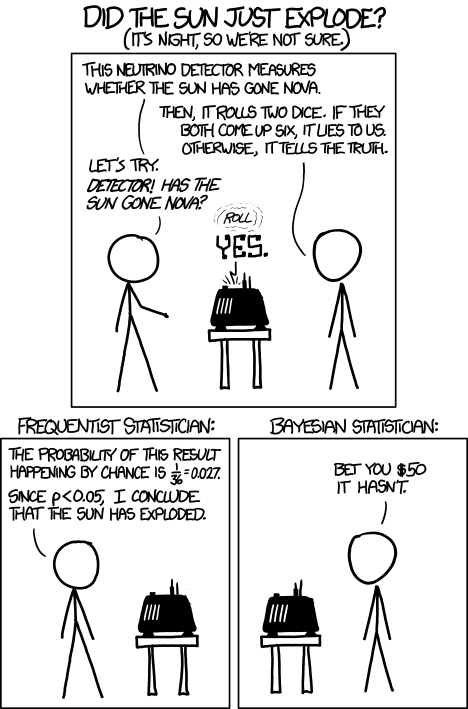
\includegraphics[scale=0.5]{../images/xkcd_frequentists_vs_bayesians}
     \caption{\textit{Source: http://xkcd.com/1132/}}
\end{figure}

\subsection{Games of Chance: Coin Toss \& Thumbtack Toss}

\subsubsection*{Coin Toss}

Alice offers Bob a bet: 
\begin{quote}
\textit{Let's toss a coin. I will give you  \$2  whenever it shows heads. But each time it shows tails, you will give me \$3.}
\end{quote}
Should Bob accept? Let's take Bob's point of view and see.
\begin{align*}
x \in \{0 = tails, 1 = heads\}\\
\mbox{If }x = 1: \mbox{Alice gives Bob \$2.}\\
\mbox{If }x = 0: \mbox{Bob gives Alice \$3.}
\end{align*}

If they play once, the money Bob gains equals: $2x - 3 (1 - x)$, with $x = 0$ on tails or $x = 1$ for heads, respectively.
But since they will play $n$ times Bob has to calculate the sum for $n$ games:
\begin{align*}
\frac{1}{n} \sum\limits_{i=1}^n \left(2x_i-3\left(1-x_i\right)\right) &= 2\left(\frac{1}{n}\sum\limits_{i=1}^n x_i\right)-3\left(\frac{1}{n}\sum\limits_{i=1}^n \left(1-x_i\right)\right)\\
&= 2\left(\frac{1}{n}\sum\limits_{i=1}^n x_i\right)-3\left(1-\frac{1}{n}\sum\limits_{i=1}^n x_i\right)
\end{align*}

Where $\frac{1}{n}\sum\limits_{i=1}^n x_i$ is the \textbf{relative proportion of heads}.\\
The expected value\index{Expected Value} (\textit{read as: ``Bob's expected gain''}) is, as can be seen above, $E = 2p - 3 (1 - p)$, where $p$ is the probability of heads.
$p$ can now easily be expressed as:
\begin{align*}
\lim_{n\rightarrow\infty}\left(\frac{1}{n}\sum\limits_{i=1}^n x_i\right) = p
\end{align*}

But what shall Bob do now, where he has a formula to derive p? Basically he has two choices: Trying out and tossing a coin $n$ times or using his \textit{a priori belief} and assigning a $p$.
How he decides is the difference between the frequentist and the Bayesian view. 
Eventually Bob sets $p = 0.5$ and inserts it into the formula for the expected outcome.
So Bob's expected gain is $E = 2 \cdot 0.5 - 3 (1 - 0.5) = -0.5 \! \left[ \$ \right] $. Hence Bob shouldn't play.

\subsubsection*{Thumbtack Toss}
\label{example:Thumbtack Toss}
Alice has another bet for Bob:
\begin{quote}
\textit{Let's toss a thumbtack. I have heads, you have tails. You are allowed to choose your stakes, but I have to agree on them to play.}
\end{quote}
What stakes should Bob choose?
We will have a look at his situation again.
\begin{align*}
x \in \{0 = tails, 1 = heads\}
\end{align*}
\begin{figure}[ht]
  \centering
  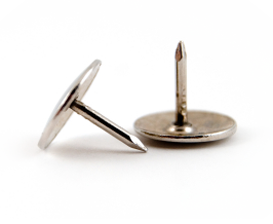
\includegraphics[scale=0.5]{../images/thumbtacks}
  \caption{Thumbtacks - left: tails, right: heads. \textit{Source: http://blog.sls-construction.com/}}
\end{figure}

The probability $p$ is again:
\begin{align*}
\lim_{n\rightarrow\infty}\left(\frac{1}{n}\sum\limits_{i=1}^n x_i\right) = p
\end{align*}

What is different is Bob's expected gain. He now has to consider the stakes as well.
\begin{align*}
E = s_1 p - s_2 (1 - p)
\end{align*}

$s_1$ is Alice's stake and $s_2$ is Bob's stake. To have a \textit{``fair''} bet the expected gain should be zero. Bob uses this knowledge to derive his stake.
\begin{align*}
& \: E = s_1 p - s_2 (1 - p)\\
0 = E \: \Leftrightarrow & \: s_1 p = s_2 (1 - p)\\
\Leftrightarrow & \: \frac{p}{1-p} = \frac{s_2}{s_1}
\end{align*}

This last formula $\frac{p}{1-p} = \frac{s_2}{s_1}$ are the \textbf{odds}\index{Odds}. If Bob fixes one stake and inserts $p$, he can calculate the other stake needed for a fair bet. But again he has the problem of how to get to $p$.

\subsubsection*{Conclusion}
To derive $p$ you always have two possibilities: The frequentist view and the Bayesian view. The difference is how we measure $p$:
\begin{itemize}
	\item \textbf{Frequentist:} measure $p$ as a property of the coin/thumbtack by throwing it $n$ times
  \item \textbf{Bayesian:} measure $p$ as a property of the ``agent'' (i.e. the decision-maker) by asking which bets are ``fair'' for him/her
\end{itemize}

\end{document}
\clearpage

% Practice: Probability Refresher I
\iftoggle{exercises}{
  
\includepdf[pages={-},
      addtotoc={1,section,1,Tutorial Sheet 1: Probability Refresher I,exsheet1},
      viewport=100 50 550 700,
      scale=0.75,
      pagecommand=\thispagestyle{plain}
      ]{exercises/Exercises01.pdf}
}{}
\iftoggle{solutions}{
  \documentclass[../main/Notes.tex]{subfiles}
\begin{document}

\section[Solution 1: Probability Refresher I]{Solution 1: Probability Refresher I \iftoggle{showdates}{\small{\textit{2014-04-28}}}{}}

\subsection*{Exercise 2}
\index{Odds}

\subsubsection*{Exercise 2.a}

We use the formula for calculating odds:
\begin{align*}
\frac{p}{1-p} = \frac{s_2}{s_1}
\end{align*}
The probability for rolling a 6 is $\frac{1}{6}$, $s_1$ can be set to 10.
\begin{align*}
\frac{\frac{1}{6}}{1-\frac{1}{6}} = \frac{s_2}{10} \Leftrightarrow s_2 = 2
\end{align*}
So our stake should be \$2.


\subsubsection*{Exercise 2.b}
We use the same formula again, this time with $s_1=25$.
\begin{align*}
\frac{\frac{1}{6}}{1-\frac{1}{6}} = \frac{s_2}{25} \Leftrightarrow s_2 = 5
\end{align*}
So we accept all stakes $s_2 \geq \$ 5$.


\subsubsection*{Exercise 2.c}
We use the formula for odds and solve it for $p$.
\begin{align*}
                & & \frac{p}{1 - p} & = \frac{s_2}{s_1}                     & & \\
\Leftrightarrow & & p               & = \frac{s_2}{s_1} (1 - p)             & & \\
\Leftrightarrow & & p               & = \frac{s_2}{s_1} - \frac{s_2}{s_1} p & & \\
\Leftrightarrow & & p s_1           & = s_2 - p s_2                         & & \\
\Leftrightarrow & & p s_1 + p s_2   & = s_2                                 & & \\
\Leftrightarrow & & p (s_1 + s_2)   & = s_2                                 & & \\
\Leftrightarrow & & p               & = \frac{s_2}{s_1 + s_2}               & &
\end{align*}
So the probability should be $p = \frac{s_2}{s_1 + s_2}$.

\subsection*{Exercise 3}
\index{Expected Value}
The average amount of juice over all trials shall be 1 ml. The formula for this 
is the known:
\begin{align*}
EV = s_1 p_1 + s_2 p_2
\end{align*}
Where $p_1$ is the probability for a red trial and $p_2$ for a blue trial. 
Since we always have either a red or a blue trial, we get the following:
\begin{align*}
EV = 1 \  ml &= s_1 p_1 + s_2 (1 - p_1)\\
\Leftrightarrow s_1 &= \frac{1 \  ml - s_2 (1 - p_1)}{p_1}\\
\Leftrightarrow s_2 &= \frac{1 \  ml - s_1 p_1}{1 - p_1}
\end{align*}
In order to obtain concrete values we need to fix $p_1$ and one of the stakes 
(either $s_1$ or $s_2$) with a value $\leq 1 \  ml$.


\subsection*{Exercise 4}
In general the statements with a conjunction are less likely. So a possible order could be:\\
$(c)\Rightarrow(d)\Rightarrow(e)\Rightarrow(f)\Rightarrow(a)\Rightarrow(b)\Rightarrow(g)$

However, many people would assign higher probabilities to those statements with conjunctions (for example ``Linda is a bank teller and is active in the feminist movement.'' is often seen as more probable than ``Linda is a bank teller.'') because of their contextual knowledge. This phenomenon is called ``conjunction fallacy''\index{Conjunction Fallacy}.

\subsection*{Exercise 5}
{\footnotesize Note: We call the \textit{set of memorized squares} $M$, the 
\textit{set of all squares} $N$ and their respective \textit{numbers of elements} 
$|M| = m$ and $|N| = n$. We also introduce $c$, the changing square, for which 
by definition holds $c \in N$.}

In this experiment we have two cases. The first case is that the number $m$ of 
squares the subject can memorize exceeds or is equal to the number $n$ of total 
squares. This case is trivial: The subject will (under ideal circumstances) 
always report the right square. Hence the probability $P(right | N \leq M) = 1$.

The second case is the more interesting case. How is the probability for being 
right if $N > M$ ($P(right | N > M)$)?

We have to distinguish between two cases again: The first case is that the 
changing square is among those $m$ squares the subject memorized, $c \in M$. 
The second case is when the change lies outside, $c \notin M$.

In the first case the subject will again always report the right $c$, but in the
second case it has to guess \textit{one out of those squares it did not memorize}.

Since we can not tell how big $M$ and $N$ are, we can not set probabilities for 
our first decision. But we can tell how big the probabilities are that $c \in M$ 
or $c \notin M$. For $c \in M$ this is simply $p = \frac{m}{n}$, we can understand 
this formula as \textit{``there are $m$ possibilities that $c$ is among the $m$ 
squares out of $N$''}. For $c \notin M$ we can just use the complementary event:
$p = 1 - \frac{m}{n}$.

We don't have to follow $c \in M$ further, as we already found out the subject 
will find the change. In case $c \notin M$ the probabilities are a bit different: 
The subject now has to pick one of the elements out of $N \setminus M$, since it 
knows that $c \notin M$. Either it hits the correct one ($p = \frac{1}{n - m}$)
or not ($p = 1 - \frac{1}{n - m}$).

All probabilities can be seen in the tree in figure \ref{tree} (page \pageref{tree}).
\index{Probability tree}
\begin{figure}
  % Set the overall layout of the tree
\tikzstyle{level 1}=[level distance=1.0cm, sibling distance=4.5cm]
\tikzstyle{level 2}=[level distance=1.5cm, sibling distance=2.5cm]
\tikzstyle{level 3}=[level distance=3.0cm, sibling distance=2.0cm]

% Define styles for bags and leafs
\tikzstyle{bag} = [text width=4em, text centered]
\tikzstyle{end} = [circle, minimum width=3pt, fill, inner sep=0pt]

% The sloped option gives rotated edge labels. Personally
% I find sloped labels a bit difficult to read. Remove the sloped options
% to get horizontal labels. 
\begin{tikzpicture}[grow=right, sloped]
\node[bag] {}
    child {
        node[bag] {$N > M$}      
            child {
                node[bag] {$c \notin M$}
                    child {
                        node[end, label=right: {$P(wrong | N > M, c \notin M)$}] {}
                        edge from parent
                        node[above] {$wrong$}
                        node[below] {$1 - \frac{1}{n - m}$}
                    }
                    child {
                        node[end, label=right: {$P(right | N > M, c \notin M)$}] {}
                        edge from parent
                        node[above] {$right$}
                        node[below] {$\frac{1}{n - m}$}
                    }
                    edge from parent
                    node[above] {}
                    node[below] {$1 - \frac{m}{n}$}
            }
            child {
                node[bag] {$c \in M$}
                    child {
                        node[end, label=right: {$P(wrong | N > M, c \in M)$}] {}
                        edge from parent
                        node[above] {$wrong$}
                        node[below] {$0$}
                    }
                    child {
                        node[end, label=right: {$P(right | N > M, c \in M)$}] {}
                        edge from parent
                        node[above] {$right$}
                        node[below] {$1$}
                    }
                    edge from parent
                    node[above] {}
                    node[below] {$\frac{m}{n}$}
            }
            edge from parent 
            node[above] {}
            node[below] {}
    }
    child {
        node[bag] {$N \leq M$}        
        child {
            node[end, label=right: {$P(wrong | N \leq M) = 0$}] {}
            edge from parent
            node[above] {$wrong$}
            node[below] {$0$}
        }
        child {
            node[end, label=right: {$P(right | N \leq M) = 1$}] {}
            edge from parent
            node[above] {$right$}
            node[below] {$1$}
        }
        edge from parent         
        node[above] {}
        node[below] {}
    };
\end{tikzpicture}

  \caption{Probability tree}
  \label{tree}
\end{figure}

To get the total probabilities for \textit{right} and \textit{wrong} choices, we 
can sum up the paths.

Note that we ignore the upper half of the tree in summing the paths up, since we 
can not derive probabilities for the first branching. We just add those cases 
individually to our function.

We get the following results:
\begin{align*}
&&P(right | N \leq M) &= 1 \\
&&P(wrong | N \leq M) &= 0 \\
&&P(right | N > M, c \in M) &= \frac{m}{n} \\
&&P(wrong | N > M, c \in M) &= 0 \\
&&P(right | N > M, c \notin M) &= \left(1 - \frac{m}{n}\right) \frac{1}{n-m} \\
&&P(wrong | N > M, c \notin M) &= \left(1 - \frac{m}{n}\right) \left(1 - \frac{1}{n-m}\right)
\end{align*}

We can now pick $P(right | N > M, c \in M)$ and $P(right | N > M, c \notin M)$ to 
calculate the marginal probability $P(right | N > M) = P(right | N > M, c \in M) + P(right | N > M, c \notin M)$.
\begin{align*}
P(right | N > M) &= \frac{m}{n} + (1 - \frac{m}{n}) \frac{1}{n - m} = \frac{m + 1}{n}
\end{align*}

Finally we can define $P_{right}(N, M)$ with $P(right | N \leq M)$ and $P(right | N > M)$:
\begin{align*}
P_{right}(N, M) = 
\begin{cases} 
1             & \mbox{if } N \leq M \\ 
\frac{|M|+1}{|N|} & \mbox{if } N > M
\end{cases}
\end{align*}

\end{document}
  \clearpage
}{}

% Probability Refresher II
\documentclass[../main/Notes.tex]{subfiles}
\begin{document}

\section[Probability Refresher II]{Probability Refresher II \iftoggle{showdates}{\small{\textit{2014-04-25}}}{}}

\subsection{Rules of Probability}
Assume a hat filled with cards. Each card has a red and a blue side, the red sides 
are labeled from 1 to 6 and blue sides from 1 to 4, resulting in 24 different cards.
We can describe this \textbf{sample space} (or \textit{set of all possible outcomes}) 
\textbf{$\Omega$} with
\begin{align*}
\Omega = \left\{ \left[ 1, 1\right], \left[ 1, 2\right], ..., \left[ 6, 4\right] \right\}
\end{align*}
where $\left[ 1, 2 \right]$ represents the card with 1 on the red and 2 on the blue side.

To describe the following examples we first have to define some terms and relations.

\begin{itemize}
	\item $x \in \Omega$ is the \textbf{random variable}\index{Random Variable} $x$ which can be drawn from $\Omega$.
    \begin{itemize}
      \item Example: $\left[ 1, 2 \right]$, i.e. the card with a red 1 and a blue 2.
    \end{itemize}
  \item $|S|$ where $S$ is a set is the \textbf{number of elements} in $S$.
    \begin{itemize}
      \item Example: $|\left\{1,2\right\}| = 2$
    \end{itemize}
  \item $E \subset \Omega$ is an \textbf{Event}\index{Event} $E$ (\textit{something you can bet on}).
    \begin{itemize}
      \item Example: Drawing a card with the number on the red site smaller than number on its blue site.
    \end{itemize}
\end{itemize}

How many events do we have? The number of events is simply $2^{|\Omega|} = 2^{24} 
= 2^{10} \cdot 2^{10} \cdot 2^4 \approx 16\mbox{ Mio}$.

If we now put another $\left[ 1, 1\right]$ card into the hat, the \textit{number of events stays the same, but the probabilities change}. This can be seen in the following table \ref{tab:2014-04-25_cards}.

\begin{table}[ht]
	\centering
    \begin{tabular}{cc|*{6}{c|}}
      \cline{3-8}
                                                  &   & \multicolumn{6}{ c| }{red}                                                                          \\ \cline{3-8}
                                                  &   & 1              & 2              & 3              & 4              & 5              & 6              \\ \cline{1-8}
      \multicolumn{1}{|c|}{\multirow{4}{*}{blue}} & 1 & $\frac{2}{25}$ & $\frac{1}{25}$ & $\frac{1}{25}$ & $\frac{1}{25}$ & $\frac{1}{25}$ & $\frac{1}{25}$ \\ \cline{2-8}
      \multicolumn{1}{|c|}{}                      & 2 & $\frac{1}{25}$ & $\frac{1}{25}$ & $\frac{1}{25}$ & $\frac{1}{25}$ & $\frac{1}{25}$ & $\frac{1}{25}$ \\ \cline{2-8}
      \multicolumn{1}{|c|}{}                      & 3 & $\frac{1}{25}$ & $\frac{1}{25}$ & $\frac{1}{25}$ & $\frac{1}{25}$ & $\frac{1}{25}$ & $\frac{1}{25}$ \\ \cline{2-8}
      \multicolumn{1}{|c|}{}                      & 4 & $\frac{1}{25}$ & $\frac{1}{25}$ & $\frac{1}{25}$ & $\frac{1}{25}$ & $\frac{1}{25}$ & $\frac{1}{25}$ \\ \cline{1-8}
\end{tabular}
	\caption{Probabilities of drawing a specific card from the hat}
	\label{tab:2014-04-25_cards}
\end{table}

To get the probability of an event we just have to sum up the values in table 
\ref{tab:2014-04-25_cards}. For example for the event ``The red number is smaller 
than the blue number'', let's call it $R < B$, the probability $P(R < B)$ can be 
calculated as follows:

\begin{align*}
P(R < B) &= P(R=1, B=2) + P(R=1, B=3) + P(R=2, B=3) \\
         &+ P(R=1, B=4) + P(R=2, B=4) + P(R=3, B=4) \nonumber \\
         &= 6 \cdot \frac{1}{25} = \frac{6}{25}
\end{align*}



\subsection{Axioms of Probability}
\begin{description}
	\item[1.] $P(\left\{\right\}) = 0, P(\Omega) = 1$
            \\ The probability for the empty set is 0. The probability for any event to happen is 1.
  \item[2.] $\forall E: 0 \leq P(E) \leq 1$
            \\ Probabilities are in the range from 0 to 1.
  \item[3.] \texttt{if $E = E_1 \cup E_2$ and $E_1 \cap E_2 = \left\{ \right\}$
            then $P(E) = P(E_1 \cup E_2) = P(E_1) + P(E_2)$}
            \\ If two events don't intersect their combined probability is the sum of their individual probabilities.
  \item[3'.] \textit{(follows from 3)} \\
            \texttt{if $E = \bigcup\limits_{i=1}^n E_i$ and $\forall_{i, j; i \neq j} E_i \cap E_j = \left\{ \right\}$ \\
            then $P(E) = P\left(\bigcup\limits_{i=1}^n E_i\right) = \sum\limits_{i=1}^{n}{P\left(E_i\right)}$}
            \\ If $n$ events don't intersect their combined probability is the sum of their individual probabilities.
\end{description}

Note that we can calculate $P$ for all events by adding up singleton events.

\subsubsection*{Other rules that follow}
\begin{figure}[ht]
  \begin{center}
    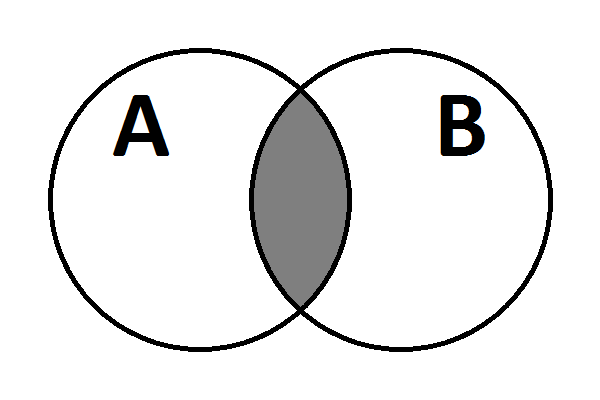
\includegraphics[scale=0.3]{../images/venn_diagram_a_intersects_b}
    \caption{The intersection between two sets makes math a bit tricky}
    \label{fig:venn_a_inter_b}
  \end{center}
\end{figure}

\begin{description}
  \item[1.] $P(A \cup B) = P(A) + P(B) - P(A \cap B) = P(A \setminus B) + P(A \cap B) + P(B \setminus A)$
            \\ The probability that one of two events happens is their individual probabilities minus the probability that both events happen simultaneously (otherwise we would account for that case twice, see also figure \nolinebreak\ref{fig:venn_a_inter_b}).
  \item[2.] $P(A \cup \neg A) = P(\Omega) = 1 = P(A) + P(\neg A)$
            \\ The probability that an event happens or not is 1.
  \item[3.] $P(A) = 1 - P(\neg A)$
            \\ The probability of an event to not happen is 1 minus the probability of the event (and vice versa).
\end{description}

\subsection{Random Variables \& Joint Distribution}
\index{Joint Distribution}\index{Random Variable}
An example for a joint distribution: You roll two dice, one is six-sided and red, the other one is four-sided and blue.
\begin{align*}
\mbox{R: }\Omega_R = \{1, ..., 6\} & & P(R=\omega) = \frac{1}{6}\ \forall\ \omega \in \Omega_R\\
\mbox{B: }\Omega_B = \{1, ..., 4\} & & P(B=\omega) = \frac{1}{4}\ \forall\ \omega \in \Omega_B
\end{align*}
The joint sample space $\Omega$ is $\Omega = \Omega_R \times \Omega_B$.

Since R and B are independent the joint probability\index{Joint Probability} is $ P(R, B) = \frac{1}{24}$ for each value of R, B.

More formally speaking it holds that $P(R=i, B=j) = \frac{1}{24}$ for all values of $i, j$ since $P(R, B) = P(R) \cdot P(B)$ for all independent $R, B$.



\subsection{Marginal and Conditional Probability}
For the following examples please refer to table \ref{tab:2014-04-25_cards} (page \pageref{tab:2014-04-25_cards}).

\subsubsection*{Marginal Probability}
The \textbf{Marginal Probability}\index{Marginal Probability} for $P(R=j)$ is:
\begin{align*}
P(R=j) = 
\begin{cases} 
\frac{5}{25} & \mbox{if } j = 1 \\ 
\frac{4}{25} & \mbox{else}
\end{cases}
\end{align*}

This can be calculated by summing up one dimension of the table.
\begin{align*}
P(R=j) = \sum\limits_{i \in \Omega_B} P(R=j, B=i)
\end{align*}

This can be written a bit more casual (here for B now):
\begin{align*}
P(B) = \sum\limits_R P(R, B) = 
\begin{cases} 
\frac{7}{25} & \mbox{if } B = 1 \\ 
\frac{6}{25} & \mbox{else}
\end{cases}
\end{align*}

\subsubsection*{Conditional Probability}
\index{Conditional Probability}In case a card was picked and we already know what number the red side shows,
$P(R, B) \neq P(R) \cdot P(B)$ is \textit{not independent}\index{Independence}. $P(R,B)$ is now dependent\index{Dependence} on the already known red number.

The probabilities that follow are:
\begin{align*}
P(B|R=1) =
\begin{cases} 
\frac{2}{5} & \mbox{if } B = 1 \\ 
\frac{1}{5} & \mbox{else}
\end{cases}\\
P(B|R=2, ..., 6) = \frac{1}{4}
\end{align*}

The conditional probability $P(A|B)$ (read: $P$ of $A$ given $B$) can be expressed as follows:
\begin{align*}
P(A|B)         &= \frac{P(A, B)}{\sum\limits_A P(A, B)} = \frac{P(A, B)}{P(B)} \\
\mbox{where}   & \\
P(A, B)        &\mbox{ is the joint pobability} \\
\sum\limits_A P(A, B) &\mbox{ is the marginal probability} \\
P(A, B)        &\mbox{ is a function of A (because B is fixed)}\\
P(B)           &\mbox{ is the renorm}
\end{align*}

With the product rule\index{Product Rule} $P(A|B)P(B) = P(A, B) = P(B|A)P(A)$ we can derive \textbf{Bayes' rule}\index{Bayes' Rule}:
\begin{align*}
P(B|A) &= \frac{P(A|B)P(B)}{P(A)} = \frac{P(A|B)P(B)}{\sum\limits_B P(A|B)P(B)} \\
\mbox{where we call}   & \\
P(B|A)  &\mbox{ posterior} \\
P(A|B)  &\mbox{ likelihood} \\
P(B)    &\mbox{ prior} \\
P(A)    &\mbox{ evidence}
\end{align*}

\end{document}
\clearpage

% Practice: Probability Refresher II
\iftoggle{exercises}{
  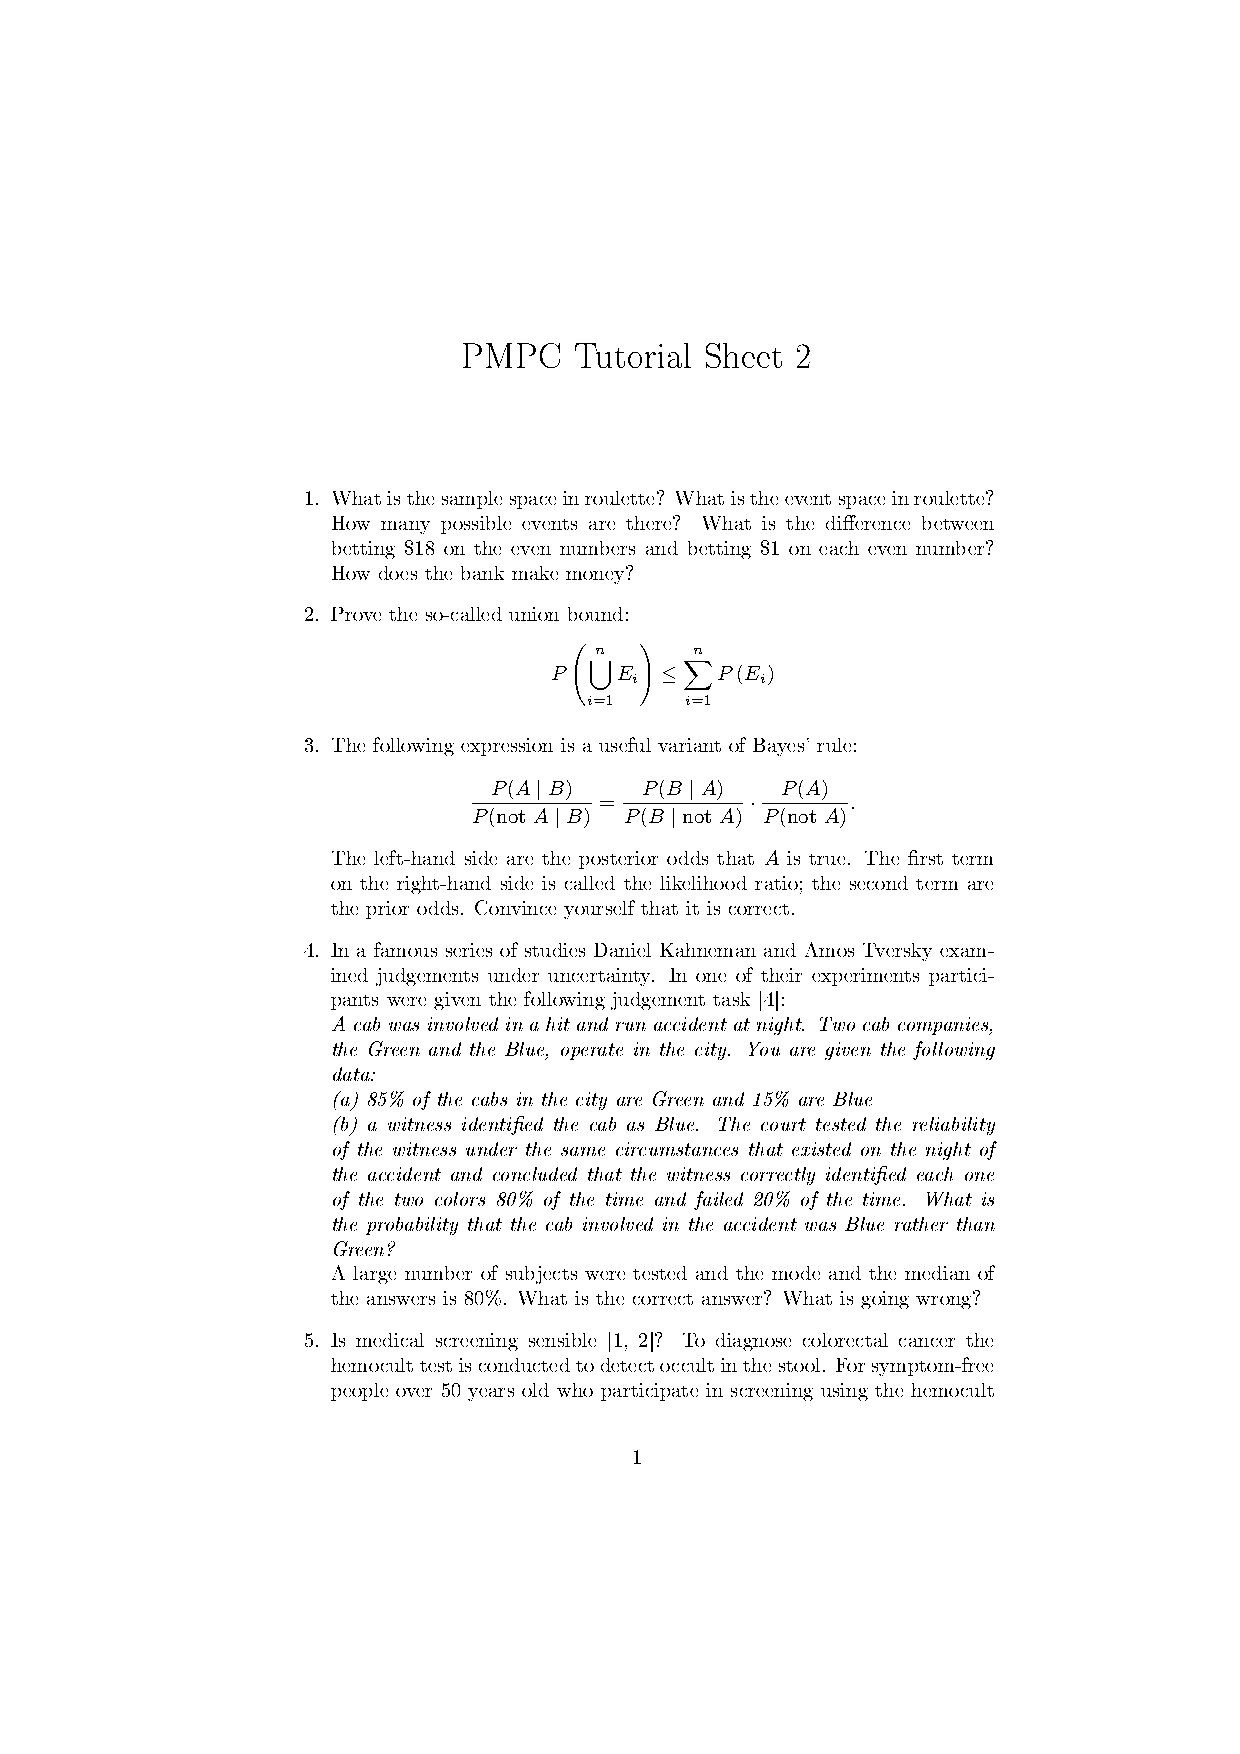
\includepdf[pages={-},
      addtotoc={1,section,1,Tutorial Sheet 2: Probability Refresher II,exsheet2},
      viewport=100 50 550 700,
      scale=0.75,
      pagecommand=\thispagestyle{plain}
      ]{exercises/Exercises02.pdf}
}{}
\iftoggle{solutions}{
  \documentclass[../main/Notes.tex]{subfiles}
\begin{document}

\section[Solution 2: Probability Refresher II]{Solution 2: Probability Refresher II \iftoggle{showdates}{\small{\textit{2014-05-05}}}{}}

\subsection*{Exercise 1}
\index{Expected Value}
There are different types of roulette, we will only deal with the so-called 
``European'' one, which features only one $0$, no $00$.

The sample space $\Omega$ is $\Omega=\left\{0, 1, 2, 3, ..., 36\right\}$. The event space is $\mathcal{P} \left( \Omega \right) \setminus \Omega$, the number of events $2^{|\Omega|} = 2^{37} = 2^{10} \cdot 2^{10} \cdot 2^{10} \cdot 2^7 \approx 128,000,000,000\ (128\ \text{Bio})$.

The expected values are:
\begin{align*}
E(even) &= 18 \cdot \frac{18}{37} - 18 \cdot \frac{19}{37} = -0.49\\
E(even\ numbers) &= \left(35 \cdot \frac{1}{37} - 1 \cdot \frac{36}{37} \right) \cdot 18 = -0.49
\end{align*}
So basically both variants are the same. 

\bigskip

\sidenote{This paragraph is from our homework research. In the lecture we just dealt with the scenario above.}
However, in European roulette there usually exists the so-called ``en prison''-rule. This rule freezes (``imprisons'') the stakes made on the small bets (``odd'', ``even'', ``red'', ``black'', ``high'', ``low'') when $0$ comes up until the specific bet was fulfilled twice in a row. When it came up twice in a row, you are allowed to get your stakes back. Alternatively, if you want to play with your bets, you can keep half of them instead of letting them being frozen, losing the other half. This modifies the expected value (assuming \textit{return} and \textit{freeze} are used with a chance of $0.5$):
\begin{align*}
E(even, 0, freeze) &= 18 \cdot \frac{18}{37} - 18 \cdot \frac{18}{37} - 0 \cdot \frac{1}{37} = 0  \\
E(even, 0, return) &= 18 \cdot \frac{18}{37} - 18 \cdot \frac{18}{37} - 9 \cdot \frac{1}{37} = -0.24  \\
E(even, 0) &= \frac{1}{2} \left( E(even, 0, return) + E(even, 0, freeze) \right) = -0.12 \\
E(even) &= \frac{\frac{1}{37} E(even, 0) + \frac{36}{37} E(even, \neg 0)}{2} = -0.48
\end{align*}

With the ``en prison'' rule betting on ``even'' is therefore better than betting on all even numbers.

\bigskip

The bank makes money because of the $0$: For calculating the odds they assume not 37 but 36 numbers.


\subsection*{Exercise 2}
\setcounter{equation}{0}
The union-bound can be proved by induction.

\bigskip

\begin{samepage}
\textbf{Induction assumption}
\begin{align}
& & P\left(\bigcup\limits_{i=1}^{n}E_i\right) & \leq \sum\limits_{i=1}^{n}(P(E_i)) & &
\end{align}
\end{samepage}

\begin{samepage}
\textbf{Base case} \\
For $n=1$ we have
\begin{align}
& & P\left(\bigcup\limits_{i=1}^{1}E_i\right) & \leq \sum\limits_{i=1}^{1}(P(E_i)) & & \\
\Leftrightarrow & & P(E_1) & \leq P(E_1) & & 
\end{align}
\end{samepage}

\begin{samepage}
\textbf{Inductive Step} \\
We know that $P(A \cup B) = P(A) + P(B) - P(A \cap B)$, so it follows that:
\begin{align}
P\left(\bigcup\limits_{i=1}^{n+1}E_i\right) &= P\left(\bigcup\limits_{i=1}^{n}E_i\right) + P(E_{n+1}) - P\left(\bigcup\limits_{i=1}^{n}E_i \cap E_{n+1}\right) \\
                                            &\stackrel{\text{IA}}{\leq} \sum\limits_{i=1}^{n}(P(E_i)) + P(E_{n+1}) = \sum\limits_{i=1}^{n+1}(P(E_i))
\end{align}
\end{samepage}

\subsection*{Exercise 3}
\index{Bayes' Rule}
\begin{align*}
P(A|B)      & = \frac{P(B|A)P(A)}{P(B)} \\
P(\neg A|B) & = \frac{P(B|\neg A)P(\neg A)}{P(B)}
\end{align*}
Putting it together:
\begin{align*}
\frac{P(A|B)}{P(\neg A|B)} = \frac{P(B|A)}{P(B|\neg A)} \frac{P(A)}{P(\neg A)}
\end{align*}

This is like:
\begin{align*}
Posterior\ Odds\ =\ Likelihood\ Ratio\ \cdot\ Prior\ Odds
\end{align*}
We can say this is updating your beliefs with new information.


\subsection*{Exercise 4}
\index{Bayes' Rule}
We use Bayes' rule to calculate $P(\text{Blue Car}|\text{Testified by Witness})$
\begin{align*}
P(B|T) = \frac{P(T|B)P(B)}{P(T)}
\end{align*}

We know that $P(T|B) = 0.8$ and $P(B) = 0.15$, so we only have to find out $P(T)$. Therefore we marginalize over B:
\begin{align*}
\sum_{B}{P(T|B)P(B)} = 0.8 \cdot 0.15 + 0.2 \cdot 0.85 = 0.29
\end{align*}

Now we can take our values and calculate the correct answer:
\begin{align*}
P(B|T) = \frac{P(T|B)P(B)}{P(T)} = \frac{0.8 \cdot 0.15}{0.29} = 0.414
\end{align*}

When testing a large group of people, the common mistake becomes obvious: they take the probability that the witness correctly identified the color, which is 80 \%. This is because they neglect the base rate (\textit{base rate neglect}\index{Base Rate Neglect}).


\subsection*{Exercise 5}
\index{Bayes' Rule}
We take Bayes' rule to calculate $P(\mbox{Cancer}|\mbox{Positive Test})$
\begin{align*}
P(C|P) = \frac{P(P|C)P(C)}{P(P)}
\end{align*}

We know that $P(P|C) = 0.5$ and $P(C) = 0.003$, so we only have to find out $P(P)$. Therefore we marginalize over C:
\begin{align*}
\sum_{C}{P(P|C)P(C)} = 0.5 \cdot 0.003 + 0.03 \cdot 0.997 = 0.0314
\end{align*}

Now we can take our values and calculate the correct answer:
\begin{align*}
P(C|P) = \frac{P(P|C)P(C)}{P(P)} = \frac{0.5 \cdot 0.003}{0.0314} = 0.048
\end{align*}

As we can see, only 4.8 \% of the people being tested positively actually have cancer. Nevertheless screening is a good thing because out of 1000 detections still 50 have cancer and those can be treated which probably makes up for the disadvantage of having 950 false alarms.  

\subsection*{Exercise 6}
\index{Bayes' Rule}
\textbf{$P(P, C)$}
\begin{tabular}{ r|c|c|l }
\multicolumn{1}{r}{}
      &  \multicolumn{1}{c}{Cancer}
               &  \multicolumn{1}{c}{$\neg$ Cancer} \\
               \cline{2-3}
Positive Test  & $\frac{15}{10,000}$ & $\frac{  300}{10,000}$     & $\frac{  315}{10,000}$\\ 
               \cline{2-3}
Negative Test  & $\frac{15}{10,000}$ & $\frac{9,670}{10,000}$     & $\frac{9,685}{10,000}$\\
               \cline{2-3}
\multicolumn{1}{r}{} 
      & \multicolumn{1}{c}{$\frac{30}{10,000}$} 
              & \multicolumn{1}{c}{$\frac{9,970}{10,000}$}
                      & \multicolumn{1}{c}{$\frac{10,000}{10,000}$}\\
\end{tabular}

\textbf{$P(P|C)$}
\begin{tabular}{ r|c|c|l }
\multicolumn{1}{r}{}
      &  \multicolumn{1}{c}{Cancer}
               &  \multicolumn{1}{c}{$\neg$ Cancer} \\
               \cline{2-3}
Positive Test  & $\frac{15}{30}$ & $\frac{ 300}{9,970}$     & \\ 
               \cline{2-3}
Negative Test  & $\frac{15}{30}$ & $\frac{9,670}{9,970}$     & \\
               \cline{2-3}
\multicolumn{1}{r}{} 
      & \multicolumn{1}{c}{$1$} 
              & \multicolumn{1}{c}{$1$} 
                      & \multicolumn{1}{c}{}\\
\end{tabular}

\textbf{$P(C|P)$}
\begin{tabular}{ r|c|c|l }
\multicolumn{1}{r}{}
      &  \multicolumn{1}{c}{Cancer}
               &  \multicolumn{1}{c}{$\neg$ Cancer} \\
               \cline{2-3}
Positive Test  & $\frac{15}{300 + 15}$   & $1 - \frac{15}{300+15}$  & $1$\\ 
               \cline{2-3}
Negative Test  & $\frac{15}{15 + 9,670}$ & $\frac{9,670}{15+9,970}$ & $1$\\
               \cline{2-3}
\multicolumn{1}{r}{} 
      & \multicolumn{1}{c}{} 
              & \multicolumn{1}{c}{} 
                      & \multicolumn{1}{c}{}\\
\end{tabular}

\textbf{Assume independence $P(C, P)$}

$P(C|P) = P(C)$

\begin{tabular}{ r|c|c|l }
\multicolumn{1}{r}{}
      &  \multicolumn{1}{c}{Cancer}
               &  \multicolumn{1}{c}{$\neg$ Cancer} \\
               \cline{2-3}
Positive Test  & $\frac{15+300}{10,000}\cdot\frac{15+15}{10,000}$   & $\frac{15+300}{10,000}\cdot\frac{300+9,670}{10,000}$  & $\frac{15+300}{10,000}$\\ 
               \cline{2-3}
Negative Test  & $\frac{15+9,670}{10,000}\cdot\frac{15+15}{10,000}$ & $\frac{15+9,670}{10,000}\cdot\frac{300+9,670}{10,000}$ & $\frac{15+9,670}{10,000}$\\
               \cline{2-3}
\multicolumn{1}{r}{} 
      & \multicolumn{1}{c}{} 
              & \multicolumn{1}{c}{} 
                      & \multicolumn{1}{c}{}\\
\end{tabular}

\subsection*{Exercise 7}
\index{Monthy Hall Problem}
As the probability for each door to contain a car is equal we know that our chance to win is given by $P(\mbox{Win}) = \frac{1}{3}$.
Further the probability that the Quiz-master chooses one of the remaining doors is $P(\mbox{Open}) = \frac{1}{2}$
The Quiz-master would not open the door which contains the car, so $P(\mbox{notOpen}|\mbox{Win}) = 1$.

Now if calculate the probability of the car being behind the unopened door using Bayes' we get:
\begin{align*}
P(Win|notOpen) = \frac{P(notOpen|Win) \cdot P(Win)}{P(notOpen)} = \frac{1 \cdot \frac{1}{3}}{\frac{1}{2}} = \frac{2}{3}
\end{align*}

Therefore the probability that the car is behind the door that the Quiz-master did not open is $\frac{2}{3}$ while the probability of our first chosen door still is $\frac{1}{3}$. So we would double our chances to win by changing our choice.

\end{document}
  \clearpage
}{}

% Measuring Beliefs I
\documentclass[../main/Notes.tex]{subfiles}
\begin{document}

\section[Measuring Beliefs I]{Measuring Beliefs I \iftoggle{showdates}{\small{\textit{2014-05-02}}}{}}

% TODO: Someone has to think over this section and write some better text. This clearly is not enough.
\subsection{Probability as Belief}
We can measure probabilities for recurring events, how can we measure probabilities for unique events?

Unique events are for example:
\begin{itemize}
	\item How sure are people which population is bigger, the EU or the US population?
  \item How can bookmakers set the odds for soccer games?
  \item How high is the probability for a nuclear reactor to blow up?
\end{itemize}

The frequentist view is not really helpful here: Since those events don't appear numerous times, you can not measure any limits of relative frequencies. But the Bayesian view helps us to use the same math to determine these probabilities.

\subsection{What do you accept as a fair bet?}\index{Fair Bet}
\begin{figure}[ht]
  \begin{center}
    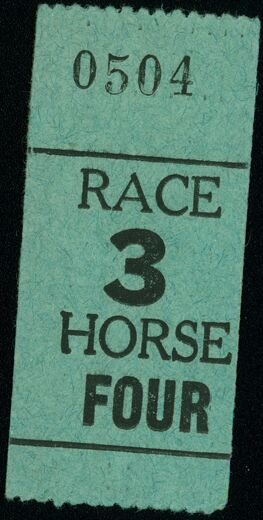
\includegraphics[]{../images/Oronsay-Rick-Danley-Horse-Race-ticket-June-30.jpg}
    \caption{A horse race ticket. \textit{Source: Reuben Goossens, ssmaritime.com}}
    \label{fig:raceticket}
  \end{center}
\end{figure}

Let's assume for the next examples that people are honest (Otherwise they would lie to win).

Assume you have a ticket you can exchange for \$1 if A happens, otherwise it's worth nothing.

\begin{align*}
Ticket = 
  \begin{cases}
    \$1 \mbox{ if } A \\
    \$0 \mbox{ else}
  \end{cases}
\end{align*}

What would be a fair price for that ticket?
\begin{align*}
\left(\$1 - c\right) P(A) - cP(\neg A) &= 0 \\
\Leftrightarrow P(A) &= c
\end{align*}

\subsubsection*{Coherence (fair pricing)}\index{Coherence}
\begin{enumerate}
	\item $P(certain) = 1$, $P(impossible) = 0$
  \item $\forall A\ 0 \leq P(A) \leq 1$
  \item $P(A \cap B) = \left\{\right\} \rightarrow P(A \cup B) = P(A) + P(B)$
\end{enumerate}

These rules follow from some logical thoughts.

Imagine $P(A) + P(\neg A) > 1$. Then the bookmaker would make money and the bet wasn't fair. If you are not the bookmaker, you want to have something like $P(A) + P(\neg A) < 1$.

Another case is $A \cap B = \left\{\right\}$, i.e. $A$ and $B$ are mutually exclusive. Then you want to buy $P(A)+P(B)$ but sell $P(A \cup B)$ if $P(A) + P(B) < P(A \cup B)$.

\subsection{Conditional Bets}
If we don't have repeatable events, how can we justify conditional probabilities\index{Conditional Probability}?

Assume a ticket again, this time of the following form:
\begin{align*}
Ticket = 
  \begin{cases}
    \$1 \mbox{ if } A \cap B \\
    \$c \mbox{ if } \neg B \mbox{\textit{(refund)}} \\
    \$0 \mbox{ else}
  \end{cases}
\end{align*}

A is dependent on B now.
% Here I also have 
% \begin{align*}
%   P(A|B) \mbox{ if }\neg B \\
%   P(\neg B) \cdot P(A|B)
% \end{align*}
% but I don't know how to explain it
\begin{align*}
P(A|B)     &=       P(A \cap B)          + P(\neg B) P(A|B) \\
         1 &= \frac{P(A \cap B)}{P(A|B)} + 1 - P(B)         \\
      P(B) &= \frac{P(A \cap B)}{P(A|B)}                    \\
P(A|B)P(B) &=       P(A \cap B)                             \\
P(A|B)     &= \frac{P(A \cap B)}{P(B)}
\end{align*}

\subsection*{Philosophical differences matter}
Alice has two coins, coin 1 with a probability of 0.5 for heads and tails, coin 2 with probability 0.4 for heads (and 0.6 for tails). 

She chooses a coin and tells Bob she would flip it $n$ times now. Then Bob has to guess which coin she flipped.

Bob has two hypotheses, one for each coin. To check his hypotheses, he can now use the data (i.e. the $n$ coin flips) and calculate the probabilities for his hypotheses - then he can compare those and choose the one with higher probability.
\begin{align*}
P(H|D) = \frac{P(D|H)P(H)}{P(D)}
\end{align*}
\textit{(with H = Hypothesis, D = Data)}

\subsection*{Calibration and Coherence}\index{Calibration}\index{Coherence}
\sidenote{In short: Being ill-\-ca\-li\-bra\-ted means you lose money on average, while being incoherent means you lose it.}
Note that there is a difference between coherence and calibration.
You are well calibrated if you answer according to your real beliefs and knowledge. For example if you play Roulette you do bet although you know that you can lose because of the 0, so you are not well calibrated (a well calibrated person in that case would not play). 
Being coherent means that you follow the rules of probability, for example that you don't trip into the conjunction fallacy trap\index{Conjunction Fallacy} (see the chapter about ``Conditional Bets'' above).

\end{document}
\clearpage

% Practice: Measuring Beliefs I
\iftoggle{exercises}{
  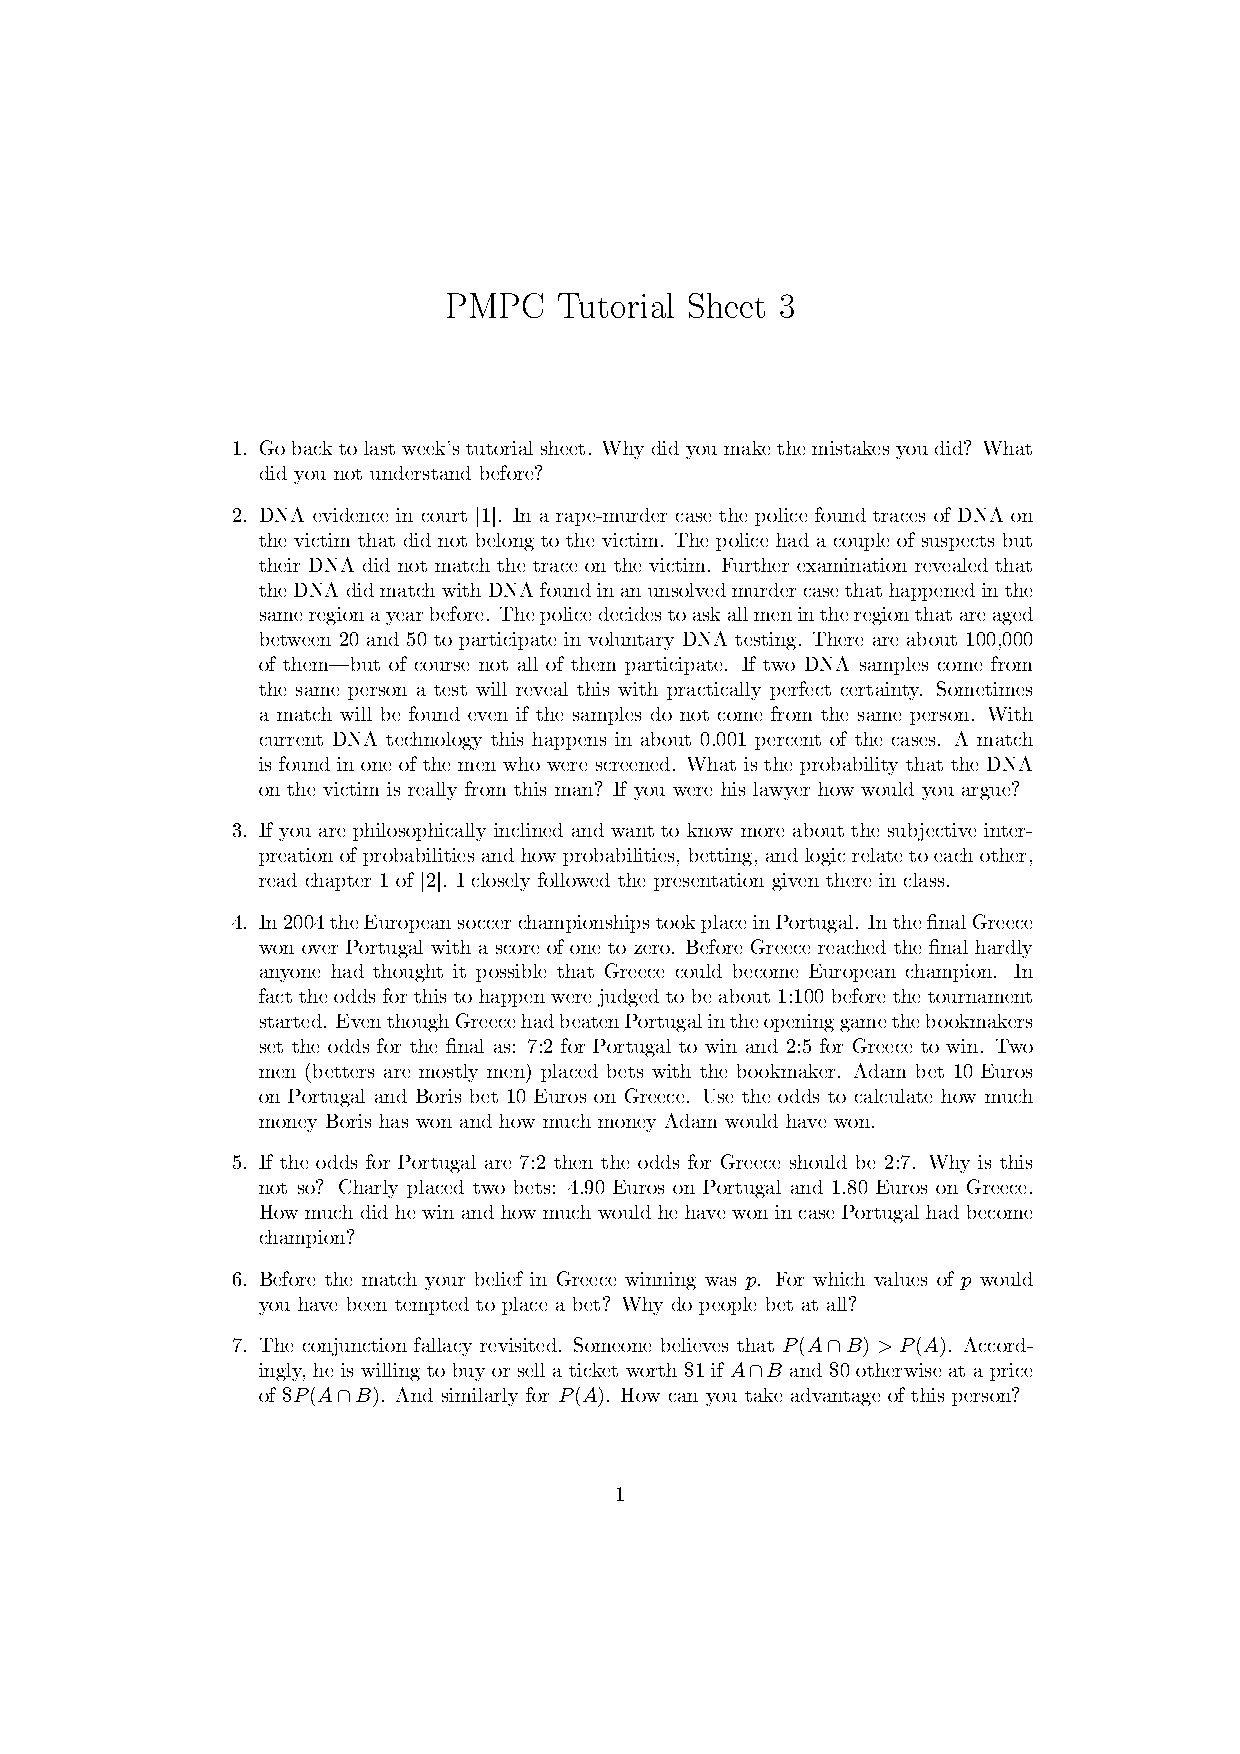
\includepdf[pages={-},
      addtotoc={1,section,1,Tutorial Sheet 3: Measuring Beliefs I,exsheet3},
      viewport=100 50 550 700,
      scale=0.75,
      pagecommand=\thispagestyle{plain}
      ]{exercises/Exercises03.pdf}
}{}
\iftoggle{solutions}{
  \documentclass[../main/Notes.tex]{subfiles}
\begin{document}

\section[Solution 3: Measuring Beliefs I]{Solution 3: Measuring Beliefs I \iftoggle{showdates}{\small{\textit{2014-05-19}}}{}}

\subsection*{Exercise 2}
\index{Bayes' Rule}
Before we can calculate any probabilities, we make some assumptions about the circumstances of the case. 

First we assume the number of subjects taking part in the DNA test is still 100,000. 

Further we assume that the murderer really is one of the men tested (and not an outsider or deceased or...) which renders the probability of being guilty ($P(G)$) as
\begin{align*}
P(G) = \frac{1}{100,000}
\end{align*}

and therefore
\begin{align*}
P(\neg G) = \frac{99,999}{100,000}
\end{align*}

A positive match with the correct DNA (i.e. matching the guilty person) has the probability of $P(P|G) = 1$.

The actual probability we are interested in is the one of really being guilty given a positive test result:
\begin{align*}
P(G|P) &= \frac{P(P|G) \cdot P(G)}{P(P)} \\
P(G|P) &= \frac{1 \cdot \frac{1}{100,000}}{P(P)}
\end{align*}

To get the missing factor, $P(P)$ we can use the marginal probability\index{Marginal Probability}:
\begin{align*}
P(P) &= \sum\limits_{i=1}^{N} \left( P(P|G_i) \cdot P(G_i) \right) \\
     &= P(P|G) \cdot P(G) + P(P|\neg G) \cdot P(\neg G) \\
     &= 1 \cdot \frac{1}{100,000} + 0.00001 \cdot \frac{99,999}{100,000} \\
     &= \frac{1.99999}{100,000}
\end{align*}

Now we can calculate $P(G|P)$:
\begin{align*}
P(G|P) &= \frac{1 \cdot \frac{1}{100,000}}{\frac{1.99999}{100,000}} = \frac{1}{1.99999} > \frac{1}{2}
\end{align*}

That means the actual probability that the accused person really is guilty is slightly above 50 \%. At first glance in court it may seem very likely that the defendant is the murderer. But we as clever attorneys can argue that with 100,000 participants taking part in the DNA test, the chance for a false alarm is still pretty high, even though the test is so accurate. This is again a case of neglecting the base rate\index{Base Rate Neglect}. 

\bigskip

Of course the probability of 50 \% is just an upper bound and can be much less for fewer participants but nevertheless shows the huge mistake one makes by neglecting the effect of a high base rate.  

\subsection*{Exercise 4}
Boris bet $10\euro$ on Greece with odds of $2 : 5$. The bookmaker bet $10\cdot\frac{5}{2}\euro=25\euro$ on Portugal. Boris won $35\euro$, which is a gain of $25\euro$.

Adam bet $10\euro$ on Portugal with odds of $7 : 2$. The bookmaker bet $10\cdot\frac{2}{7}\euro=2.86\euro$ on Greece. Adam would have won $12.86\euro$, which would have been a gain of $2.86\euro$.

\subsection*{Exercise 5}
\index{Expected Value}\index{Odds}
Charly's bets were $4.90\euro+1.80\euro=6.70\euro$ in total.

\begin{align*}
E(Portugal) &= 4.90 \cdot \frac{2}{7} - 1.80 = -0.4 {[}\euro{]} \\
E(Greece)   &= 1.80 \cdot \frac{7}{2} - 4.90 =  1.4 {[}\euro{]}
\end{align*}

If the odds\index{Odds} were a fair bet\index{Fair Bet}, i.e. $7 : 2$ for Portugal and $2 : 7$ for Greece, Charly had either lost $0.40\euro$ in case Portugal won, or he'd gained $1.40\euro$ in case Greece won.

\bigskip

The bookmaker however wants to make money, that's why he fixes the odds in a way that he will earn some.

\begin{itemize}
	\item[] With $7 : 2$ for Portugal Charly's gain in case of Portugal's victory will be $4.90 \cdot \frac{2}{7} - 1.80 = -0.40 {[}\euro{]}$, he in fact loses money.
  \item[] With $2 : 5$ for Greece Charly's gain in case of Greece's victory will be $1.80 \cdot \frac{5}{2} - 4.90 = -0.40 {[}\euro{]}$, again he loses money in total.
\end{itemize}

So the bookmaker would always win some money (those $0.40 \euro$ Charly lost in each case).

\subsection*{Exercise 6}
\begin{align*}
& \frac{p}{1-p} \geq \frac{2}{5}\\
& \Leftrightarrow 5p \geq 2 - 2p\\
& \Leftrightarrow 7p \geq 2\\
& \Leftrightarrow p \geq \frac{2}{7}
\end{align*}
If the probability for Greece to win was higher than $\frac{2}{7}$, we might have been tempted to place a bet.

People bet because they hope to win or assume they have a dutch book\index{Dutch Book} (i.e. a guaranteed win). And they will bet if they really have a dutch book.

To check if a dutch book is possible one can do a simple calculation:
\begin{align*}
\frac{7}{7+2} + \frac{2}{2+5} \stackrel{?}{<} 1 \\
\end{align*}
That is checking if the probabilities from the bookmaker's view are less or greater than 1. If they are greater, you will lose - if their sum is smaller, you can find a dutch book.


\subsection*{Exercise 7}
\index{Conjunction Fallacy}
The person believes that $P(A \cap B)>P(A)$.

We can buy cheap $P(A)$ tickets and sell expensive $P(A\cap B)$ tickets, so even before we know the outcome we make money.

In practice now the other person has $P(A \cap B)$, we have $P(A)$.

Now we see what could happen:
\begin{align*}
     A \cap      B:& \mbox{ We are even.}      \\
     A \cap \neg B:& \mbox{ I get \$ 1.}       \\
\neg A \cap      B:& \mbox{ All tickets lose.} \\
\neg A \cap \neg B:& \mbox{ All tickets lose.}
\end{align*}

So either both parties have the same outcome or we win.

\subsection*{Exercise 8}
\index{Geometric Distribution}
\textit{Note: pin $:= 1-p$, head $:= p$}

The sample space is $\Omega = \mathbb{N}$ because we can get pin on the first, second, third, or $n$-th throw.

We calculate the probability distribution.
\begin{align*}
p(N = n) = p^{n - 1} \left( 1 - p \right)
\end{align*}

We can use \textit{countable additivity}\index{Countable Additivity} and add the numbers up to infinity.
\begin{align*}
1 &\stackrel{?}{=} \sum\limits_{n = 1}^\infty p(N = n) = \sum\limits_{n = 1}^\infty p^{n - 1}\left( 1 - p \right) \\
&= \left( 1 - p \right) \sum\limits_{n=0}^\infty p^n = \left( 1 - p \right) \frac{1}{\left( 1 - p \right)} \stackrel{!}{=} 1
\end{align*}

For odd $N$ the probability is accordingly:
\begin{align*}
P\left(\mbox{N is odd}\right) &= \sum\limits_{n=0}^\infty p(N=2n+1)\\
&= \sum\limits_{n=0}^\infty \left( 1 - p \right) p^{2n} \\
&= \left( 1 - p \right) \sum\limits_{n=0}^\infty \left(p^2\right)^n \\
&= \frac{1-p}{1-p^2} = \frac{1}{1+p}
\end{align*}

\subsection*{Exercise 9}
\index{St. Petersburg Paradox|(}
\begin{tabular}{ l || c | c | c | c | c }
  $N$           & $1$ & $2$ & $3$ & $...$ & $n$ \\
  $probability$ & $\frac{1}{2}$ & $\frac{1}{4}$ & $\frac{1}{2^3}$ & $...$ & $\frac{1}{2^n}$ \\
  $Win$         & $2^1$ & $2^2$ & $2^3$ & $...$ & $2^n$ \\
\end{tabular}

The probability that we lose money is for all $N$ where we get less than 1000 \$.
\begin{align*}
2^N > 1000 \rightarrow N \geq 10 \\
p\left(\mbox{lose money}\right) = p(N<10) = \sum\limits_{n=1}^9 \frac{1}{2^n} \approx 0.998
\end{align*}

Now the expected gain is:
\begin{align*}
E &= -1000 + \frac{1}{2} \cdot 2^1 + \frac{1}{4} \cdot 2^2 + \frac{1}{8} \cdot 2^3 + ... \\
  &= -1000 + \sum\limits_{n=1}^\infty \frac{1}{2^n} \cdot 2^n \\
  &= -1000 + \sum\limits_{n=1}^\infty 1 \\
  &= +\infty
\end{align*}

Although this looks rather promising, of course we don't play the game.
\index{St. Petersburg Paradox|)}
% maybe some details about logarithmic value of money etc.?

\subsection*{Exercise 10}
We just check with which model (i.e. with which die) the given data set is more probable - that is the best guess we can make.

\begin{align*}
P(min|D) &= \frac{P(D|min)P(min)}{P(D)} \\
P(red|D) &= \frac{P(D|red)P(red)}{P(D)} \\
P(red)   &= \frac{1}{2}  \\
P(min)   &= \frac{1}{2}  \\
P(D|min) &= \frac{5}{36} 
      + 2 \cdot \left(\frac{9}{36}\right)
      + \frac{3}{36}
      + 4 \cdot \left( \frac{1}{36} \right)
      + \frac{7}{36}
      + \frac{11}{36}
      = \frac{48}{36} = \frac{4}{3} \\
P(D|red) &= 10 \cdot \left(\frac{1}{6}\right) = \frac{10}{6} = \frac{5}{3}
\end{align*}

$P(D|min) < P(D|red)$, so she most probably decided on the red die.

\end{document}
  \clearpage
}{}

% Measuring Beliefs II
\documentclass[../main/Notes.tex]{subfiles}
\begin{document}

\section[Measuring Beliefs II]{Measuring Beliefs II \iftoggle{showdates}{\small{\textit{2014-05-09}}}{}}

\subsection{Probabilities of Continuous Random Variables}\index{Continuous Random Variable}
How tall is Frank Jäkel? 1.80m, 1.70m, 1.68m, 1.69m, or even 1.7034241m?

Not only are there problems with real numbers like 1.7034241, but also with the question the Bayesian view inevitably asks: ``What do you think is the probability for that size?''

One sees: continuous random variables are difficult. There is an infinite uncountable range of numbers and one shall assign probabilities for them. This leads straight to the question: ``What's the probability of a real number?''

In the following section this problem gets tackled in three ways.

\subsubsection[Probability Density Function (PDF)]{Solution 1: Histograms (Probability Density Function, PDF)}\index{PDF}
The first and naive way is to discretize the sample space $\mathbb{R}$ into bins and assign probabilities to those bins (figure \ref{fig:2014-05-09_Histogram}).

\begin{figure}[!ht]
\centering
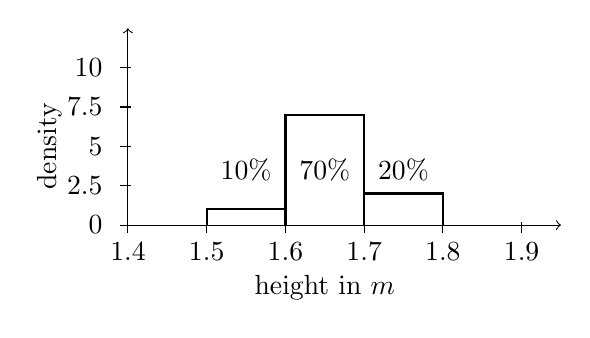
\begin{tikzpicture}

  % horizontal axis
  \draw[->] (0, 0) -- (5.5, 0);
  % ticks horizontal
  \foreach \x in {0,...,5}
    \draw (\x,1pt) -- (\x,-3pt);
  % labels horizontal
  \draw	(0,-0.1) node[anchor=north] {1.4}
		    (1,-0.1) node[anchor=north] {1.5}
		    (2,-0.1) node[anchor=north] {1.6}
		    (3,-0.1) node[anchor=north] {1.7}
		    (4,-0.1) node[anchor=north] {1.8}
		    (5,-0.1) node[anchor=north] {1.9}
        ;
  % axis label
  \draw (2.5,-0.8) node {height in $m$};
  
  % vertical axis
  \draw[->] (0, 0) -- (0, 2.5);
  % ticks vertical
  \foreach \y in {0,0.5,1,1.5,2}
    \draw (1pt, \y) -- (-3pt, \y);
  % labels vertical
  \draw (-0.2,0.0) node[anchor=east]  {0}
        (-0.2,0.5) node[anchor=east]  {2.5}
        (-0.2,1.0) node[anchor=east]  {5}
        (-0.2,1.5) node[anchor=east]  {7.5}
        (-0.2,2.0) node[anchor=east] {10}
        ;
  % axis label
  \draw (-1,1) node[rotate=90] {density};
  
  % first box
  \draw[thick] (1, 0) -- (1, 0.2) -- (2, 0.2) -- (2, 0);
  % second box
  \draw[thick] (2, 0) -- (2, 1.4) -- (3, 1.4) -- (3, 0);
  % third box
  \draw[thick] (3, 0) -- (3, 0.4) -- (4, 0.4) -- (4, 0);
  
  % box labels
  \draw (1.5, 0.7) node{$10 \%$};
  \draw (2.5, 0.7) node{$70 \%$};
  \draw (3.5, 0.7) node{$20 \%$};
  
\end{tikzpicture}
\caption{Histogram}
\label{fig:2014-05-09_Histogram}
\end{figure}

Note that \textbf{the area describes the probability}. For the second box, one would assign a y-value of 7, such that the width (0.1) times the height equals the probability ($0.1\cdot 7 = 0.7$).

For a finer granularity one can now change the resolution of the bins and split the probabilities among them (figure \ref{fig:2014-05-09_fineHistogram}.

\begin{figure}[!ht]
\centering
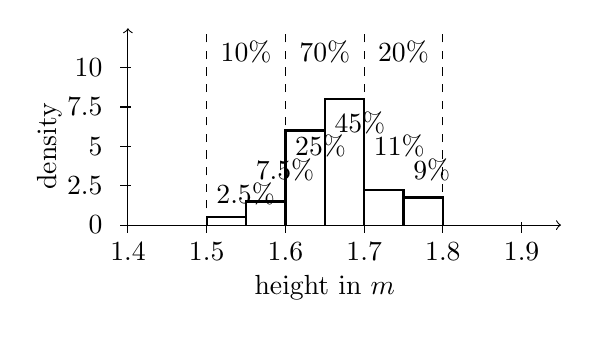
\begin{tikzpicture}

  % horizontal axis
  \draw[->] (0, 0) -- (5.5, 0);
  % ticks horizontal
  \foreach \x in {0,...,5}
    \draw (\x,1pt) -- (\x,-3pt);
  % labels horizontal
  \draw	(0,-0.1) node[anchor=north] {1.4}
		    (1,-0.1) node[anchor=north] {1.5}
		    (2,-0.1) node[anchor=north] {1.6}
		    (3,-0.1) node[anchor=north] {1.7}
		    (4,-0.1) node[anchor=north] {1.8}
		    (5,-0.1) node[anchor=north] {1.9}
        ;
  % axis label
  \draw (2.5,-0.8) node {height in $m$};
  
  % vertical axis
  \draw[->] (0, 0) -- (0, 2.5);
  % ticks vertical
  \foreach \y in {0,0.5,1,1.5,2}
    \draw (1pt, \y) -- (-3pt, \y);
  % labels vertical
  \draw (-0.2,0.0) node[anchor=east]  {0}
        (-0.2,0.5) node[anchor=east]  {2.5}
        (-0.2,1.0) node[anchor=east]  {5}
        (-0.2,1.5) node[anchor=east]  {7.5}
        (-0.2,2.0) node[anchor=east] {10}
        ;
  % axis label
  \draw (-1,1) node[rotate=90] {density};
  
  % first box
  \draw[thick] (1.0, 0) -- (1.0, 0.1) -- (1.5, 0.1) -- (1.5, 0);
  \draw[thick] (1.5, 0) -- (1.5, 0.3) -- (2.0, 0.3) -- (2.0, 0);
  % second box
  \draw[thick] (2.0, 0) -- (2.0, 1.2) -- (2.5, 1.2) -- (2.5, 0);
  \draw[thick] (2.5, 0) -- (2.5, 1.6) -- (3.0, 1.6) -- (3.0, 0);
  % third box
  \draw[thick] (3.0, 0) -- (3.0, 0.45) -- (3.5, 0.45) -- (3.5, 0);
  \draw[thick] (3.5, 0) -- (3.5, 0.35) -- (4.0, 0.35) -- (4.0, 0);
  
  % box labels
  \draw (1.5, 2.2) node{$10 \%$};
  \draw (2.5, 2.2) node{$70 \%$};
  \draw (3.5, 2.2) node{$20 \%$};
  
  \draw (1.0, 0.4) node[anchor=west]{$2.5 \%$};
  \draw (1.5, 0.7) node[anchor=west]{$7.5 \%$};
  \draw (2.0, 1.0) node[anchor=west]{$25 \%$};
  \draw (2.5, 1.3) node[anchor=west]{$45 \%$};
  \draw (3.0, 1.0) node[anchor=west]{$11 \%$};
  \draw (3.5, 0.7) node[anchor=west]{$ 9 \%$};
  
  % vertical separation lines
  \draw[thin, dashed] (1, 0) -- (1, 2.5);
  \draw[thin, dashed] (2, 0) -- (2, 2.5);
  \draw[thin, dashed] (3, 0) -- (3, 2.5);
  \draw[thin, dashed] (4, 0) -- (4, 2.5);
  
\end{tikzpicture}
\caption{Histogram with higher resolution}
\label{fig:2014-05-09_fineHistogram}
\end{figure}

\begin{samepage}
\textbf{Extreme cases}
Usually this will yield a nice distribution of how beliefs are. However, there are two special extreme cases.

\begin{enumerate}
  \item[] The first case is that all values are equally probable: Since we have infinitely many values on the real number line, the probability for each individual value is $\frac{1}{n} \Rightarrow \lim\limits_{n\rightarrow\infty} \frac{1}{n} = 0$. 
  \item[] The second case is that the full probability gets assigned to one single value. Since a single value has the width 0, again the probability will become 0 for all values.
\end{enumerate}
\end{samepage}

\textbf{The probability density function}
However, if the resulting histogram is somewhere between those extreme cases, then the limit of the distribution yields the probability density function (figure \ref{fig:2014-05-09_pdf}).

\begin{figure}[!ht]
\centering
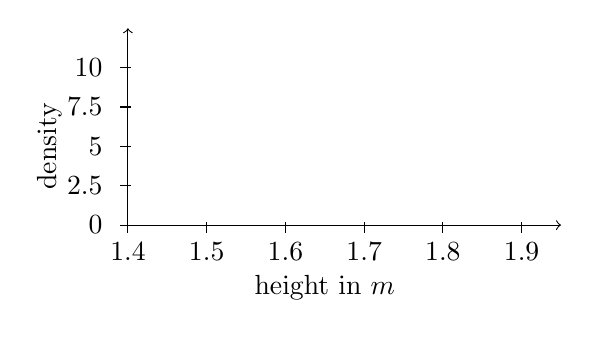
\begin{tikzpicture}
  
  % horizontal axis
  \draw[->] (0, 0) -- (5.5, 0);
  % ticks horizontal
  \foreach \x in {0,...,5}
    \draw (\x,1pt) -- (\x,-3pt);
  % labels horizontal
  \draw	(0,-0.1) node[anchor=north] {1.4}
		    (1,-0.1) node[anchor=north] {1.5}
		    (2,-0.1) node[anchor=north] {1.6}
		    (3,-0.1) node[anchor=north] {1.7}
		    (4,-0.1) node[anchor=north] {1.8}
		    (5,-0.1) node[anchor=north] {1.9}
        ;
  % axis label
  \draw (2.5,-0.8) node {height in $m$};
  
  % vertical axis
  \draw[->] (0, 0) -- (0, 2.5);
  % ticks vertical
  \foreach \y in {0,0.5,1,1.5,2}
    \draw (1pt, \y) -- (-3pt, \y);
  % labels vertical
  \draw (-0.2,0.0) node[anchor=east]  {0}
        (-0.2,0.5) node[anchor=east]  {2.5}
        (-0.2,1.0) node[anchor=east]  {5}
        (-0.2,1.5) node[anchor=east]  {7.5}
        (-0.2,2.0) node[anchor=east] {10}
        ;
  % axis label
  \draw (-1,1) node[rotate=90] {density};
  
  \draw[thick] plot[smooth] file {../data/2014-05-09_HistogramToPDF.txt};
\end{tikzpicture}
\caption{Probability density function}
\label{fig:2014-05-09_pdf}
\end{figure}

As mentioned before it's still not possible to calculate the probability of a specific number. What is possible though, is calculating the probability of an interval. This is useful, since people always bet on intervals. For instance, betting on ``2'' means to bet on the interval $\left[2,3\right[$.

\subsubsection[Cumulative Density Function (CDF)]{Solution 2: Cumulative Density Function, CDF}\index{CDF}
To calculate the probability of an interval it's possible to simply sum up all probabilities in the specific interval.

This can be done by integration of the PDF\index{PDF} (see figure \ref{fig:2014-05-09_pdf_to_cdf}).

\begin{figure}[!ht]
\centering
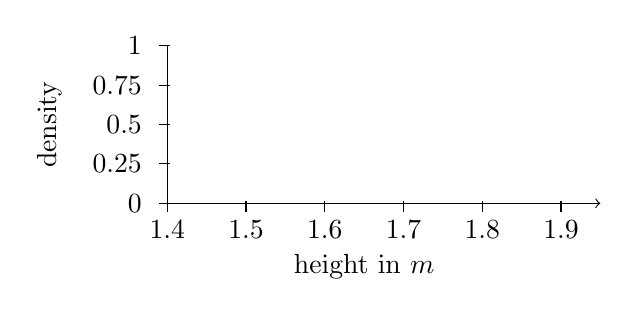
\begin{tikzpicture}
  
  % horizontal axis
  \draw[->] (0, 0) -- (5.5, 0);
  % ticks horizontal
  \foreach \x in {0,...,5}
    \draw (\x,1pt) -- (\x,-3pt);
  % labels horizontal
  \draw	(0,-0.1) node[anchor=north] {1.4}
		    (1,-0.1) node[anchor=north] {1.5}
		    (2,-0.1) node[anchor=north] {1.6}
		    (3,-0.1) node[anchor=north] {1.7}
		    (4,-0.1) node[anchor=north] {1.8}
		    (5,-0.1) node[anchor=north] {1.9}
        ;
  % axis label
  \draw (2.5,-0.8) node {height in $m$};
  
  % vertical axis
  \draw[-] (0, 0) -- (0, 2);
  % ticks vertical
  \foreach \y in {0,0.5,1,1.5,2}
    \draw (1pt, \y) -- (-3pt, \y);
  % labels vertical
  \draw (-0.2,0.0) node[anchor=east] {0}
        (-0.2,0.5) node[anchor=east] {0.25}
        (-0.2,1.0) node[anchor=east] {0.5}
        (-0.2,1.5) node[anchor=east] {0.75}
        (-0.2,2.0) node[anchor=east] {1}
        ;
  % axis label
  \draw (-1.5,1) node[rotate=90] {density};
  
  \draw[thick] plot[smooth] file {../data/2014-05-09_CDF.txt};
\end{tikzpicture}
\caption{Cumulative density function}
\label{fig:2014-05-09_pdf_to_cdf}
\end{figure}


\subsubsection[Parametric Gaussian Distribution]{Solution 3: Parametric Distribution}\index{Parametric Distribution}
The only remaining problem is deriving the correct probability density function. We can avoid this by using a very common statistics method and model the PDF\index{PDF} as a Gaussian distribution\index{Gaussian Distribution}.

This way we reduce the problem finding the correct function to finding the correct parameters.

\bigskip

The Gaussian distribution (see figure \ref{fig:2014-05-09-diffGaussDistr}) is defined as
\begin{align*}
p(X=x) = \frac{1}{2\pi\sigma^2}e^{-\frac{1}{2}\left(\frac{\mu-x}{\sigma}\right)^2} &= \phi(x;\mu,\sigma) = \phi\left(\frac{\mu-x}{\sigma};0,1\right) \\
\frac{\mu-x}{\sigma}&=z
\end{align*}

The corresponding integral is $\Phi$ (see figure \ref{fig:2014-05-09-diffGaussDistr}).
\begin{align*}
P(X \leq t) = \int\limits_{-\infty}^{t}{p(X=x)} dx &= \Phi(t;\mu,\sigma)
\end{align*}

\begin{figure}[!ht]
\centering
\begin{tikzpicture}
  \begin{axis}[every axis plot post/.append style={mark=none, domain=-4:4, samples=50, smooth}, 
    axis x line*=bottom, axis y line*=left, enlargelimits=upper, name=gauss]
    \addplot [red]    {gauss(0,0.5)};% node[pos=0.4,  anchor=east] {$\sigma=0.5$};
      \addlegendentry{$\mu=0,\sigma=0.5$}
    \addplot [green]  {gauss(0,1)};%   node[pos=0.6,  anchor=west] {$\sigma=1$};
      \addlegendentry{$\mu=0,\sigma=1$}
    \addplot [blue]   {gauss(0,2)};%   node[pos=0.85, anchor=west] {$\sigma=2$};
      \addlegendentry{$\mu=0,\sigma=2$}
    \addplot [yellow] {gauss(1,1)};%   node[pos=0.7,  anchor=west] {$\mu=1,\sigma=1$};
      \addlegendentry{$\mu=1,\sigma=1$}
  \end{axis}

  \begin{axis}[every axis plot post/.append style={mark=none, domain=-4:4, samples=50, smooth}, legend style={at={(0.98,0.02)}, anchor=south east}, 
    axis x line*=bottom, axis y line*=left, enlargelimits=upper, name=Gauss, at=(gauss.right of east), anchor=left of west]
    \addplot [red]    {Gauss(0,0.5)};% node[pos=0.5,  anchor=west] {$\sigma=0.5$};
      \addlegendentry{$\mu=0,\sigma=0.5$}
    \addplot [green]  {Gauss(0,1)};%   node[pos=0.5,  anchor=east] {$\sigma=1$};
      \addlegendentry{$\mu=0,\sigma=1$}
    \addplot [blue]   {Gauss(0,2)};%   node[pos=0.85, anchor=west] {$\sigma=2$};
      \addlegendentry{$\mu=0,\sigma=1$}
    \addplot [yellow] {Gauss(1,1)};%   node[pos=0.7,  anchor=west] {$\mu=1,\sigma=1$};
      \addlegendentry{$\mu=1,\sigma=1$}
  \end{axis}
\end{tikzpicture}
\caption{Left: Gaussian distributions. Right: Their corresponding integrals. Parameters: $\mu=0$ and $\sigma = 0.5, 1, 2$, and $\mu=1, \sigma=1$.}
\label{fig:2014-05-09-diffGaussDistr}
\end{figure}

The area of the standard deviation\index{Standard Deviation} ($\mu - \sigma \leq X \leq \mu + \sigma$) has a probability of approximately 68 \% (see figure \ref{fig:2014-05-09-std}).
\begin{align*}
P(\mu - \sigma \leq X \leq \mu + \sigma) = \Phi(\mu+\sigma;\mu,\sigma) - \Phi(\mu-\sigma;\mu,\sigma) \approx 68 \%
\end{align*}

\begin{figure}[!ht]
\centering
\begin{tikzpicture}
\begin{axis}[axis x line*=bottom, axis y line*=left, enlargelimits=upper, axis on top, domain=-4:4, y post scale=0.5]
  \addplot+[domain=-1:1, samples=100, pattern=flexible hatch, mark=none
            hatch distance=5pt, hatch thickness=0.5pt,
            draw=green, pattern color=green!40, area legend]
            {gauss(0,1)} \closedcycle;
    \addlegendentry{$\approx 68\%$}
  \addplot[color=red, samples=50, smooth] {gauss(0,1)};
    \addlegendentry{$\mu=0,\sigma=1$}
\end{axis}
\end{tikzpicture}
\caption{The area of the standard deviation yields approximately 68 \%}
\label{fig:2014-05-09-std}
\end{figure}

\begin{samepage}
We can also find other useful probabilities which are commonly used to do statistics:
\begin{itemize}
	\item $\mu \pm \sigma \approx 68\%$
	\item $\mu \pm 2\sigma \approx 95\%$
	\item $\mu \pm 3\sigma \approx 99\%$
\end{itemize}
\end{samepage}


\subsection{Proper Scoring Rules}\index{Proper Scoring Rule}
Multiple choice tests would be better if you would state ``how your belief is, that this is right'', rather than just answering the question (For more about this see page \pageref{ex4_4_solution}).

\bigskip

Take a look at this example: \\ \textit{The EU population is bigger than the US population. \\
Give the belief for this to be true. \\(This means 0 = ``I believe this is false'', 1 = ``I believe this is true'', 0.5 = ``I don't know'')}

\bigskip

The aim of a proper scoring rule is to yield a high gain (a minimum loss) if the answer is true and the belief in it is high, but yield no gain if the answer is false but the belief in it high.

In the loss-function $L$ given below $q$ is the belief assigned to the answer given and $X$ is 1 if the statement was true or 0 if it was false.
\begin{align*}
L\left(X,q\right) &= \left(X-q\right)^2 \\
                  &= X^2-2qX+q^2 \mbox{ \textit{(note: $X^2 = X$, since only 0 or 1)}} \\
                  &= X\left(1-2q\right)+q^2
\end{align*}

\subsubsection*{Penalty for lying}
If we now assume the subject is not stating her actual belief $p$, but another value $q$ ($p\neq q$), the formula changes in the following way:
\begin{align*}
E\left(L\left(p,q\right)\right) &= p-2pq+q^2 = \left(p-p^2\right) + \left(p^2-2pq+q^2\right) \\&= \underbrace{p\left(1-p\right)}_\text{basic loss} + \underbrace{\left(p-q\right)^2}_\text{penalty for lying}
\end{align*}
Note that the basic loss is maximal if the subject has no clue ($p=0.5$). 
\subsubsection*{How to answer?}
If one's belief is p, which q will yield the best gain (i.e. will minimize the expected loss)?

To answer this the expected loss\index{Expected Loss} function can be minimized, i.e. one can search the first derivative and set it to zero. 

\begin{align*}
E\left(L\left(p,q\right)\right) &= p\left(1-2q\right)+q^2 \\
\frac{\partial E\left(L\left(p,q\right)\right)}{\partial q} &= -2p + 2q \\
\rightarrow 0 &= -2p + 2q \\
\Leftrightarrow p &= q
\end{align*}

As can be seen the loss function is minimal if $p=q$, i.e. if the person answering is telling the truth.

\end{document}
\clearpage

% Practice: Measuring Beliefs II
\iftoggle{exercises}{
  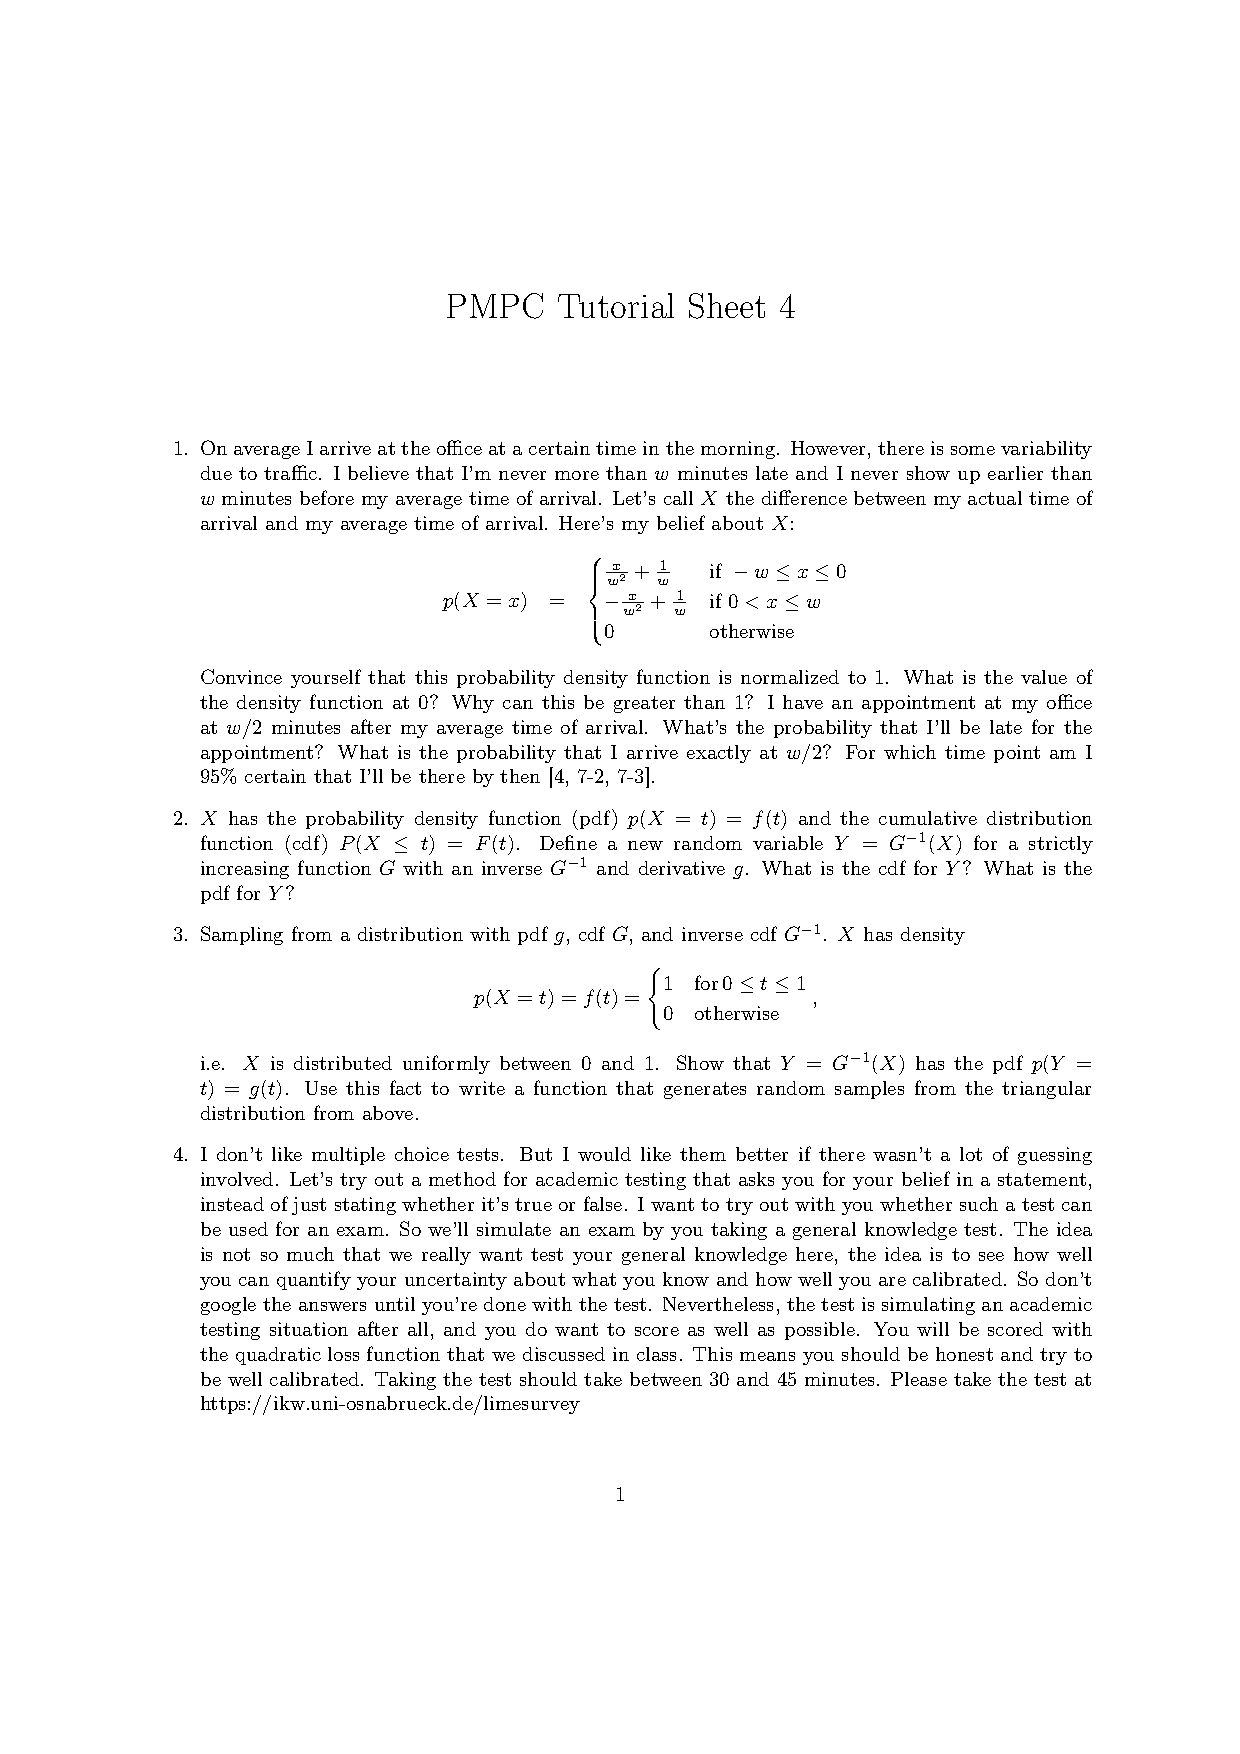
\includepdf[pages={-},
      addtotoc={1,section,1,Tutorial Sheet 4: Measuring Beliefs II,exsheet4},
      viewport=100 50 550 700,
      scale=0.75,
      pagecommand=\thispagestyle{plain}
      ]{exercises/Exercises04.pdf}
}{}
\iftoggle{solutions}{
  \documentclass[../main/Notes.tex]{subfiles}
\begin{document}

\section[Solution 4: Measuring Beliefs II]{Solution 4: Measuring Beliefs II \iftoggle{showdates}{\small{\textit{2014-05-19}}}{}}

\subsection*{Exercise 1}
In order to calculate the area under the density function we have to take the integral. As the function is defined differently for separate segments we can first calculate the integral from $-\omega$ to 0 and then from 0 to $\omega$ (the rest is zero anyways).
\begin{align*}
\int \limits_{-w}^{0}p(x) dx & = \int \limits_{-w}^{0} \frac{x}{\omega^2} + \frac{1}{w} dx \\
& =     \left[\frac{1}{2\omega ^2} \cdot x^2 + \frac{1}{\omega } \cdot x \right]_{-w}^{0} \\
& = 0 - \left(\frac{1}{2\omega ^2} \cdot \left(- \omega\right)^2 + \frac{1}{x} \cdot \left(-\omega\right) \right) \\
& = -\left(\frac{1}{2} - 1\right) \\
& = \frac{1}{2}\\
\int \limits_{0}^{\omega}p(x) dx & = \int \limits_{0}^{\omega} -\frac{x}{\omega^2} + \frac{1}{w} dx \\
& = \left(-\frac{1}{2\omega ^2} \cdot \omega^2 + \frac{1}{x} \cdot \omega\right) - 0 \\
& = -\left(\frac{1}{2} - 1\right) \\
& = \frac{1}{2}\\
\int \limits_{-\omega}^{\omega}p(x) dx & = \int \limits_{-\omega}^{0}p(x) dx +\int \limits_{0}^{\omega}p(x) dx \\
& = \frac{1}{2} + \frac{1}{2} \\
& = 1
\end{align*}

The value of the density function at 0 is given by:
\begin{align*}
p(X=0) & = \frac{1}{\omega^2} \cdot 0 + \frac{1}{\omega} = \frac{1}{\omega}
\end{align*}

Therefore the value at zero can be greater than 1 for $\omega >$ 1. This is possible because the density is not equal to the probability (which cannot be greater than 1) but has to be multiplied with the width of interval for which the probability should be calculated.

In order to get the probability for coming late at time point $\frac{\omega}{2}$ we have to calculate the probability for arriving after that time point, or in other words the integral from $\frac{\omega}{2}$ to $\omega$ (again the remaining area is zero anyways):
\begin{align*}
  p\left(X > \frac{\omega}{2}\right) &= \int\limits_{\frac{\omega}{2}}^{\omega} p(x) dx \\
  &= \int\limits_{\frac{\omega}{2}}^{\omega} -\frac{x}{\omega^2} + \frac{1}{w} dx \\
  &= \left[-\frac{1}{2\omega^2}\cdot x^2 + \frac{1}{w}\cdot x\right]_{\frac{\omega}{2}}^{\omega} \\
  &= -\frac{1}{2\omega^2}\cdot \omega^2 + \frac{1}{\omega}\cdot \omega - \left(-\frac{1}{2\omega^2}\cdot \left(\frac{\omega}{2}\right)^2 + \frac{1}{\omega}\cdot \frac{\omega}{2}\right) \\
  &= \frac{1}{2} + \frac{1}{2\omega^2}\cdot\frac{\omega^2}{4} - \frac{1}{2}\\
  &= \frac{1}{8}\\
  &= 12.5\% \\
\end{align*}

Therefore the probability to come late to the appointment is 12.5\%.

The probability to arrive exactly at time point $\frac{\omega}{2}$ on the other hand is zero, because probabilities of continuous variables can only be calculated for intervals and not for points. Or mathematically:

$\int\limits_{\frac{\omega}{2}}^{\frac{\omega}{2}} p(x)dx = 0$

As we know from the first part of the exercise, the probability to arrive before time point 0 is 50\%. Thus we can just calculate the area after 0 which makes up for 45\% to get the time point at which we can be sure with 95\%  that we will arrive before:
\begin{align*}
  \int\limits_{0}^{t} p(x)dx &\stackrel{!}{=} 0.45 \\
  \left[-\frac{1}{2\omega^2}\cdot x^2 + \frac{1}{\omega}\right]_0^t & = 0.45 \\
  -\frac{1}{2\omega^2}\cdot t^2 + \frac{1}{\omega} - 0 &= 0.45 \\
 \mbox{substitute: }z&=\frac{t}{\omega} \\
  \frac{1}{2}\cdot z^2 + z &= 0.45 \\
  z^2 - 2z &= -0.9 \\
  z^2 - 2z + 1 &= 0.1 \\
  \left(z-1\right)^2 &= 0.1 \\
  z-1 &= \sqrt{0.1} \\
  z &= \sqrt{0.1} + 1 \\
  z &= 1.3162 \vee  z = 0.6838 \\
  \frac{t}{\omega} &= 1.3162 \vee  \frac{t}{\omega} = 0.6838 \\
  t &= 1.3162\cdot \omega \vee t  = 0.6838 \cdot \omega
\end{align*}

Since we know that we have to arrive before $\omega$ it can only be the second value. Therefore we can be 95\% sure that we arrive before $0.6838 \cdot \omega$.


\subsection*{Exercise 2}
\begin{align*}
Y &= G^-1(X) \\
\mbox{cdf: }   P\left(Y \leq t\right)
             &= P\left(G^-1\left(X\right) \leq t\right) \\
             &= P\left(X \leq G\left(t\right)\right) \\
             &= F\left(G\left(t\right)\right) \\
\mbox{pdf: }   \frac{\partial F\left(G\left(t\right)\right)}{\partial t}
             &= f\left(G\left(t\right)\right) \cdot g\left(t\right)
\end{align*}

\subsection*{Exercise 3}
\begin{align*}
\mbox{pdf: } \frac{\partial F\left(G\left(t\right)\right)}{\partial t} &=f\left(G\left(t\right)\right) \cdot g\left(t\right)
\end{align*}

$f(t)$ is 1 for $0 \leq t \leq 1$, so $f\left(G\left(t\right)\right) \cdot g\left(t\right) = 1 \cdot g\left(t\right) = g\left(t\right)$.

\subsection*{Exercise 4}
See page \pageref{ex4_4_solution} for details on this exercise.

\subsection*{Exercise 5}
We can replace X with p in $L_2$ \textit{(this only works if the function is linear in X, see Tutorial Sheet 5)} and check if it's a good loss function.

First derivative:
\begin{align*}
L_2\left(X,q\right) &= -X \cdot \log{\left(q\right)} - \left(1 - X\right) \cdot \log{\left(1-q\right)} \\
E\left(L_2\left(p,q\right)\right) &= -p \cdot \log{\left(q\right)} - \left(1 - p\right) \cdot \log{\left(1-q\right)} \\
\frac{\partial E\left(L_2\left(p, q\right)\right)}{\partial q} &= -p \cdot \frac{1}{q} - \left(1 - p\right) \frac{-1}{1-q} \\
&= -\frac{p}{q} + \frac{\left(1 - p\right)}{1-q}
\end{align*}

Check for p = q:
\begin{align*}
0 &= -\frac{p}{q} + \frac{\left(1 - p\right)}{1-q} \\
\Leftrightarrow \frac{p}{q} &= \frac{1-p}{1-q} \\
\Leftrightarrow p \cdot \left(1 - q\right) &= \left(1 - p\right) \cdot q \\
\Leftrightarrow p - pq &= q - pq \\
\Leftrightarrow p &= q
\end{align*}

Second derivative:
\begin{align*}
\frac{\partial E\left(L_2\left(p, q\right)\right)}{\partial q} &= \frac{-p}{q} + \frac{1-p}{1-q} \\
\frac{\partial E\left(L_2\left(p, q\right)\right)}{\partial^2 q} &= \frac{p}{q^2} + \frac{1-p}{\left(1-q\right)^2}
\end{align*}
\begin{align*}
\text{use: } p &= q\\
\Rightarrow \frac{q}{q^2} + \frac{1-q}{\left(1-q\right)^2} &= \frac{1}{q} + \frac{1}{1-q} \\
&= \frac{1}{q-q^2} > 0
\end{align*}
Since the second derivative is greater than zero in our definition from $0...1$ we found a minimum, so the loss function is good for honest people.

Still usually the first loss function is better, since this second function is unforgiving (a single mistake gives a loss of $\infty$).

\end{document}
  \clearpage
}{}

% Bayesian Inference Examples
\documentclass[../main/Notes.tex]{subfiles}
\begin{document}

\section[Bayesian Inference Examples]{Bayesian Inference Examples \iftoggle{showdates}{\small{\textit{2014-05-23}}}{}}
\label{ex4_4_solution}
This section is basically about Exercise 4 on the 4th Tutorial Sheet (see page \pageref{exsheet4}). The idea is that we have a multiple choice test where the answers are not simply true or false but can be any value between 0 and 1 representing your belief in this statement to be true (where 0 corresponds to your belief in this statement being false, 1 that you belief it's true). What does a proper scoring do in this example? What is calibration?\index{Calibration}

\subsection{Honesty}
If we use a proper scoring rule\index{Proper Scoring Rule} the participant can minimize her error if she always states her honest belief in the statement. It is obvious that this does not help in getting any points for statements where you have no clue about its real truth value and you can still get lucky if you gamble and just guess a value for a statement. 

But for a huge number of questions it is highly unlikely that you gain anything and we proved in the other exercises that it is optimal to state your true belief.

\subsection{Calibration}\index{Calibration|(}
If you are well-calibrated then $80 \%$ of the statements you marked with $80 \%$ should be true. Calibration is the bridge between frequentist and Bayesian view on this topic. Calibration can only be measured if you have a huge enough sample space, which is not often the case since you have rather twenty than two hundred questions. 

Afterwards it is not possible (in our setup) to tell whether wrong answers are due to lying or bad calibration. There is another problem: It is very hard for a normal person to be well calibrated (even if they try). Psychological studies show that most people systematically overestimate their own belief. Meaning that they would write $1$ where their true belief is rather $0.92$. 

People also overestimate small probabilities. For example, people think that it is rather likely to die in a plane crash than in a car accident, although this is rather unlikely compared to car accidents. One could take such studies into account and try to come up with correction terms for the common failures, but this is rather complicated. This is part of the reason why these proper scoring or multiple choice tests of this form are not widely used. The other reason is that not many people know about this stuff and the effect is not that great to even start with all the trouble.
\index{Calibration|)}

\end{document}
\clearpage

% Frequentist Inference Examples
\documentclass[../main/Notes.tex]{subfiles}
\begin{document}

\section[Frequentist Inference Examples]{Frequentist Inference Examples \iftoggle{showdates}{\small{\textit{2014-05-26}}}{}}

\subsection{Bayesian Inference for Thumbtacks}
We return to the example from the first lecture (see page \pageref{example:Thumbtack Toss}). Let us imagine we have thrown a thumbtack $n$ times. The series of data we get from that may be: 01110101101, a binary string consisting of $n$ entries (0 encodes tail, 1 head). Let $x_1....x_n =: X$ be a random variable. What is the probability of the data given our vague belief about q (for a coin we have the strong intuition of believing that $q=0.5$, but for the thumbtack we are not sure)? The probability of the whole data ($X$) is the product of the probability of all single events ($x_i$):
\begin{align*}
P(X|q) = \prod\limits_{i=1}^n{\underbrace{q^{x_i}\left(1-q\right)^{1-x_i}}_\text{Bernoulli}}=q^h\left(1-q\right)^t
\end{align*}
h: \#heads
t: \#tails

But since we do not know $q$ we would also like to find the best $q$ that explains the observed data. In other words: what is the probability of a specific $q$ given the data? This can again be expressed with Bayes' Rule\index{Bayes' Rule}:
\begin{align*}
\overbrace{p(q|X)}^\text{posterior} = \frac{P(X|q)\overbrace{p(q)}^\text{prior}}{\int_0^1 P(X|q)p(q) dq}
\end{align*}

\sidenote{$\alpha,\beta\in\mathbb{N}_+$: $B(\alpha,\beta) = \frac{(\alpha-1)!(\beta-1)!}{(\alpha+\beta-1)!}$}
The question arising here is what shall we take as the prior? In principle it is just our personal belief about the thumbtack, one experimenter might believe it is $0.7$, others believe different values. This \textit{subjectivity} troubles many Non-Bayesians. The good thing is, that it does not really matter which prior you choose, if you have enough data the result will still converge to the real $p(q|X)$!

Since we have no concrete clue and it is not that important anyway, we may choose a distribution by pure convenience for $p(q)$. The distribution is called \textit{$\beta$ Distribution}\index{B@$\beta$-Distribution} :
\begin{align*}
p(q) &= \frac{q^{\alpha-1}(1-q)^{\beta-1}}{\int_0^1 q^{\alpha-1}(1-q)^{\beta-1}dq} = \frac{q^{\alpha-1}(1-q)^{\beta-1}}{B(\alpha,\beta)}
\end{align*}
We can now neglect the normalization term in the original $p(q|X)$. So we get rid of the integral in the denominator, since it is independent of $q$.
\begin{align*}
p(q|X) &\propto \underbrace{q^h(1-q)^t}_{P(X|q)} \underbrace{q^{\alpha-1}(1-q)^{\beta-1}}_{p(q)} = \underbrace{q^{h+\alpha-1}(1-q)^{t+\beta-1}}_\text{new $\beta$-distribution}
\end{align*}
If we now choose $\alpha_n = h+\alpha, \beta_n = t+\beta$, we can express the new $\beta$ Distribution as:
\begin{align*}
p(q|X) &= \frac{q^{\alpha_n-1}(1-q)^{\beta_n-1}}{B(\alpha_n, \beta_n)} 
\end{align*}

If the prior and posterior have the same distribution (like in this case) they are called \textit{conjugate}\index{Conjugation}.

\subsection{Map estimate (maximum a posteriori)}
In order to find the maximum posteriori term we need to calculate the first derivative of $p(q|X)$. That seems quite hard but we can reduce the problem by ignoring the normalization term $\frac{1}{B(\alpha_n, \beta_n)}$ (since it is independent from $q$) and taking the logarithm of the numerator, since this does not change the location of any maxima. By this we just have to maximize $\log(q^{\alpha_n-1}(1-q)^\beta_n-1)$.

\begin{align*}
\log{\left(q^{\alpha_n-1}(1-q)^{\beta_n-1}\right)} &= (\alpha_n-1)\log \est{q} + (\beta_n-1)\log (1-\est{q}) \\
\frac{\partial \left(\left(\alpha_n-1\right)\log \est{q} + \left(\beta_n-1\right)\log \left(1-\est{q}\right)\right)}{\partial \est{q}} &= \frac{\alpha_n-1}{\est{q}} - \frac{\beta_n-1}{1-\est{q}} = 0 \\
\frac{\alpha_n-1}{\est{q}} = \frac{\beta_n-1}{1-\est{q}} &\Leftrightarrow \frac{1-\est{q}}{\est{q}} = \frac{\beta_n-1}{\alpha_n-1} \\
\frac{1}{\est{q}} = \frac{\beta_n-1}{\alpha_n-1}+1 &= \frac{\beta_n-1}{\alpha_n-1} + \frac{\alpha_n-1}{\alpha_n-1} = \frac{\beta_n+\alpha_n-2}{\alpha_n-1} \\
\est{q} = \frac{\alpha_n-1}{\beta_n+\alpha_n-2} &= \frac{\alpha+h-1}{\alpha+\beta+h+t-2}
\end{align*}

\sidenote[.35]{The approach of using Bayes\-ian statistics with a prior that does not assume or put in any information is called 'Objective Bayes'. It is somehow the middle ground between the two opposing camps.}

For $\alpha = \beta = 1$ we get what we have already suspected before: $\est{q}=\frac{h}{h+t}$. $\alpha$ and $\beta$ are also called pseudo-counters. They represent data points you have not seen but believe to be realistic. This is a way to put your prior belief about the problem in the model - but it is also dangerous. If you have a strong belief in a hypothesis it will need more and more data to prove in the limit that you are wrong.



\subsection[Null Hypothesis Significance Testing (NHST)]{NHST Null Hypothesis Significance Testing}\index{NHST}
In the previous section we examined how Bayesian people tackle the problem of finding a good model for a problem. For frequentists it is a bit more complicated. Remember that probabilities (like the probability for heads for a fair coin) are objective/fixed properties of the object. Writing $p(q)$ (as well as $p(q|X) \propto p(q)p(X|q)$) makes no sense for this reason. $q$ is not a random variable but a property and we need to find out its concrete value.

\subsubsection*{Experiment: Can someone discriminate between coke and pepsi?}
\sidenote{This section is wrong and needs to be updated!}
We would like to know what $p(q)$ is. But as frequentists we can't do that. So we start with the null hypothesis $H_0$: Subjects can't discriminate: $q = \frac{1}{2}, n = 25$. Where $q$ denotes the discrimination factor for the subjects and $n$ is the number of trials. We now measure H (\# ``Heads'': correct discriminations).
\begin{align*}
P(H=h|q) = \underbrace{ \binom{n}{h} q^h (1-q)^{n-h} }_\text{Binomial distribution}\index{Binomial Distribution}
\end{align*}

\sidenote{Obviously WIP!}
Now we introduce a criterion: subjects can discriminate if they get >20 correct answers. In that case you reject the null hypothesis.

--- some gauss distribution from notes

\begin{align*}
&P\left(H=h |q=\frac{1}{2},n=25\right) \\
&P\left(H>20 |q=\frac{1}{2},n=25\right) \mbox{ (p-Value)}
\end{align*}

$\alpha$ is the signal level $\rightarrow$ type I error rate that's acceptable (usually $5\%$). This is the probability that you say there is an effect even if there is none.

say $q = \frac{4}{5}$

--- another plot from notes

type II error $\beta \approx \frac{3}{4}$

tradeoff between $\alpha$ and $\beta$: ``easier'' for $q \rightarrow \frac{1}{2}$ for $n$ big: the power is $1-\beta$.

\end{document}
\clearpage

% Practice: Bayesian and Frequentist Inference
\iftoggle{exercises}{
  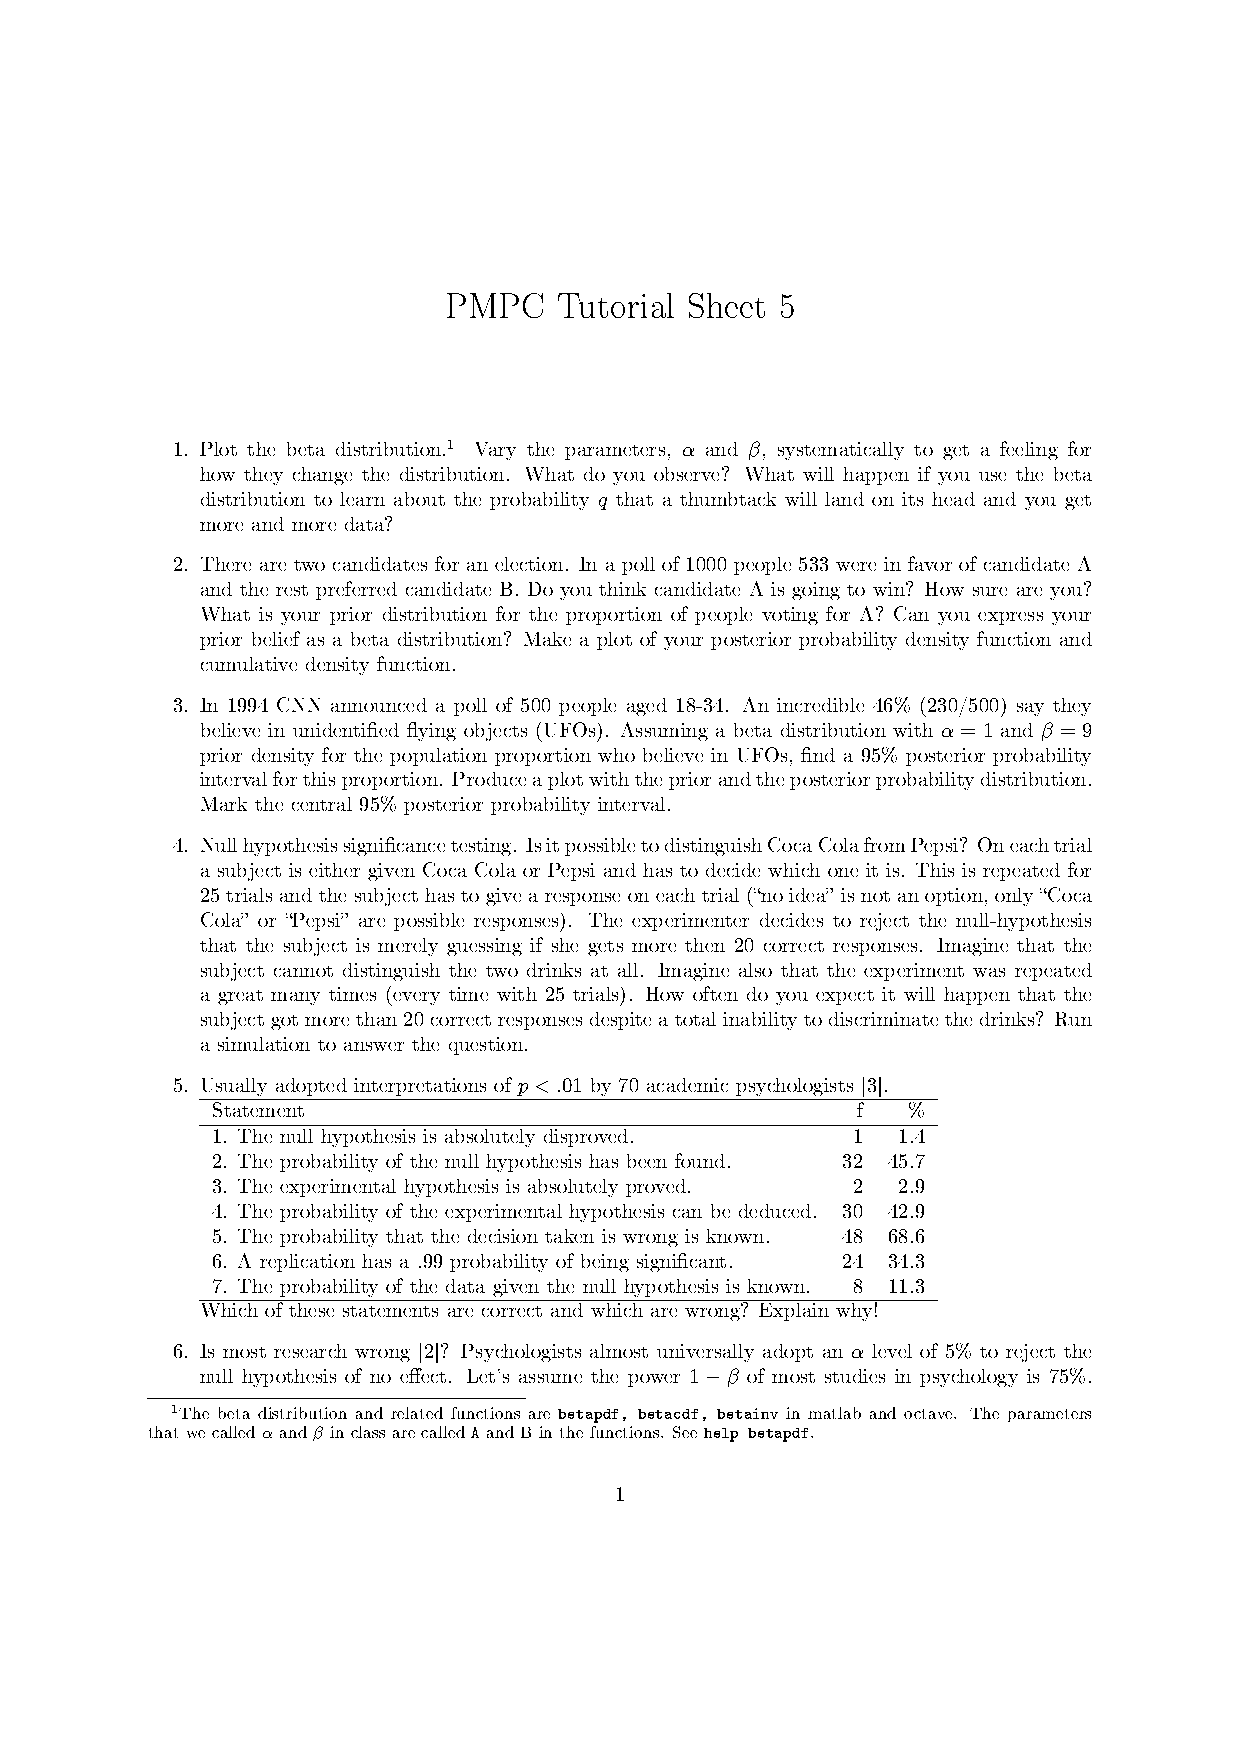
\includepdf[pages={-},
      addtotoc={1,section,1,Tutorial Sheet 5: Bayesian and Frequentist Inference I,exsheet5},
      viewport=100 50 550 700,
      scale=0.75,
      pagecommand=\thispagestyle{plain}
      ]{exercises/Exercises05.pdf}
}{}
\iftoggle{solutions}{
%  \documentclass[../main/Notes.tex]{subfiles}
\begin{document}

\section[Solution 5: Bayesian and Frequentist Inference I]{Solution 5: Bayesian and Frequentist Inference I \iftoggle{showdates}{\small{\textit{2014-05-30}}}{}}

\subsection*{Exercise 1}
\begin{figure}[!ht]
\centering
\begin{tikzpicture}
  \begin{axis}[axis x line*=bottom, axis y line*=left, enlargelimits=upper, axis on top, domain=0:1, legend style={at={(0.98,0.5)}, anchor=east}, x post scale=2, y post scale=2]
  \addplot[smooth, samples=100, color=blue]    {betaDist(1,1)};
    \addlegendentry{$\alpha=1,\beta=1$}
  \addplot[smooth, samples=100, color=purple]  {betaDist(2,2)};
    \addlegendentry{$\alpha=2,\beta=2$}
  \addplot[smooth, samples=100, color=yellow]  {betaDist(3,3)};
    \addlegendentry{$\alpha=3,\beta=3$}
  \addplot[smooth, samples=100, color=red]     {betaDist(1,2)};
    \addlegendentry{$\alpha=1,\beta=2$}
  \addplot[smooth, samples=100, color=magenta] {betaDist(1,3)};
    \addlegendentry{$\alpha=1,\beta=3$}
  \addplot[smooth, samples=100, color=orange]  {betaDist(1,5)};
    \addlegendentry{$\alpha=1,\beta=8$}
  \addplot[smooth, samples=100, color=cyan]    {betaDist(2,1)};
    \addlegendentry{$\alpha=2,\beta=1$}
  \addplot[smooth, samples=100, color=black]   {betaDist(3,1)};
    \addlegendentry{$\alpha=3,\beta=1$}
  \addplot[smooth, samples=100, color=green]   {betaDist(5,1)};
    \addlegendentry{$\alpha=8,\beta=1$}
  \addplot[smooth, samples=100, color=gray]    {betaDist(3,6)};
    \addlegendentry{$\alpha=3,\beta=6$}
  \end{axis}
\end{tikzpicture}
\caption{Different $\beta$-distributions}
\label{fig:2014-05-30_ex1betadistributions}
\end{figure}

We can easily observe that the $\beta$-distribution\index{B@$\beta$-Distribution} is symmetric for $\alpha=\beta$ and always 1 in case $\alpha=\beta=1$. If we increase one parameter the distribution's peak wanders to one side, towards 0 for higher $\beta$s and towards 1 for higher $\alpha$s.

If we increase both parameters unequally, the distribution's peak moves towards the higher parameter (similar to the movement mentioned before, see $\alpha=3,\beta=6$) and gets for high values much narrower and steeper (not shown in the plot, see figure \ref{fig:2014-05-30_ex3posterior} for an example).

\bigskip

When using the $\beta$-distribution to learn about the probability $q$ for the thumbtack example (page \pageref{example:Thumbtack Toss}) we would start with $\alpha=\beta=1$, i.e. uninformed. After gathering some data we can use it to update our prior belief and adjust the parameters according to our posterior distribution. If we continue doing this iteratively the distribution will get closer to the real $q$ of the thumbtack. % Note: We should find out which distribution we have with n throws and k successes (probably binomial)


\subsection*{Exercise 2}
We have only very limited information and a best guess is that A will win the elections, since there are 53.3\% of the people supporting him. We are not really sure about that because of the lack of information.

Our prior belief is uninformed, i.e. we have no idea about the outcome (Assuming we don't know the poll). The likelihood is our data sample, i.e. the poll's data. It is a binomial distribution\index{Binomial Distribution}: $P(Poll|A) = \binom{1000}{533} p^{533}(1-p)^{1000-533}$. We use the $\beta$-distribution\index{B@$\beta$-Distribution} to model our prior belief: it is conjugate to the Binomial distribution. 

We try to find to find $P(A|Poll)$, i.e. the probability that A wins the election given the poll results.
\begin{align*}
P(A|Poll) &= \frac{P(Poll|A)P(A)}{P(Poll)}\\
P(A|Poll) &= \frac{\binom{1000}{533}p^{533}(1-p)^{467} \cdot p^{\alpha-1}(1-p)^{\beta-1}}{B(\alpha,\beta)}\\
\text{using an uninformed prior, i.e. }\alpha=1, \beta=1\\
P(A|Poll) &= \frac{\binom{1000}{533}p^{533}(1-p)^{467} \cdot p^{1-1}(1-p)^{1-1}}{B(1,1)}\\
P(A|Poll) &\propto \frac{p^{533+1-1}(1-p)^{467+1-1}}{B(534,468)}
\end{align*}

We can plot this posterior belief $P(A|Poll)$ (figure \ref{fig:2014-05-30_ex2plot}) and see how likely it is that A wins. Since the highest density is above 0.5, it's more likely that A wins the election.
\begin{figure}[!ht]
\centering
\begin{tikzpicture}
  \begin{axis}[axis x line*=bottom, axis y line*=left, enlargelimits=upper, axis on top, domain=0:1, legend style={at={(0.98,0.5)}, anchor=east}]
  % csvwrite('2014-05-30_exercise2_pdf.txt',[[0:0.001:1]' betapdf(0:0.001:1,534,468)'])
  \addplot[smooth] file {../data/2014-05-30_exercise2_pdf.txt};
    \addlegendentry{$\genfrac{}{}{0pt}{}{\alpha=534}{\beta=468}$}
  \draw ({axis cs:0.5,0}|-{rel axis cs:0,0}) -- ({axis cs:0.5,0}|-{rel axis cs:0,1});
  \end{axis}
\end{tikzpicture}
\caption{How likely is it, that A wins the election?}
\label{fig:2014-05-30_ex2plot}
\end{figure}


\subsection*{Exercise 3}
We denote $B$ as the number of people believing in UFOs and $D$ as the data (i.e. the poll results) given.

Using the $\beta$-Distribution\index{B@$\beta$-Distribution} we come up with the following model:
\begin{align*}\index{Binomial Distribution}
                P(B|D) &= \frac{P(D|B)P(B)}{P(D)} \\
\Leftrightarrow P(B|D) &= \frac{\binom{500}{230}q^{230}\left(1-q\right)^{500-230}P(B)}{P(D)}\\
                P(B|D) &= \frac{\overbrace{\binom{500}{230}q^{230}\left(1-q\right)^{270}}^\text{Binomial} \overbrace{q^{\alpha-1}\left(1-q\right)^{\beta-1}}^\text{$\beta$-Distribution}}{B(\alpha,\beta)} \\
                P(B|D) &\propto q^{230+1-1}\left(1-q\right)^{270+9-1} \\
                P(B|D) &\Rightarrow \frac{q^{231-1}\left(1-q\right)^{279-1}}{B(231,279)}
\end{align*}

The prior distribution (figure \ref{fig:2014-05-30_ex3prior}) is far to the left, as we have a relatively huge $\beta$ compared to $\alpha$.
\begin{figure}[!ht]
\centering
\begin{tikzpicture}
  \begin{axis}[axis x line*=bottom, axis y line*=left, enlargelimits=upper, axis on top, domain=0:1]
  \plot[smooth, color=blue] file {../data/2014-05-30_priorPDF_data.txt};
    \addlegendentry{$\alpha=1,\beta=9$}
  \end{axis}
\end{tikzpicture}
\caption{Prior $\beta$-Distribution}
\label{fig:2014-05-30_ex3prior}
\end{figure}

With the new $\alpha = 231$ and $\beta = 279$ we can find the $95\%$ interval by calculating the CDF\index{CDF} of the posterior $\beta$-distribution and searching for the x-values for $y_{min}=0.025$ and $y_{max}=0.975$. Using these x-values for the corresponding PDF\index{PDF} yields the $95\%$ interval (figure \ref{fig:2014-05-30_ex3posterior}). The left figure shows the CDF and the intersections for a visual explanation: By using the inverse of the CDF we can calculate the x-values much easier.

\begin{figure}[!ht]
\centering
\begin{tikzpicture}
  \begin{axis}[axis x line*=bottom, axis y line*=left, enlargelimits=upper, axis on top, domain=0:1, name=cdf, legend style={at={(0.98,0.5)}, anchor=east}]
  \plot[smooth, color=blue] file {../data/2014-05-30_posteriorCDF_data.txt};
    \addlegendentry{$\genfrac{}{}{0pt}{}{\alpha=231}{\beta=279}$}
  \plot[color=red] {0.975};
    \addlegendentry{$x=0.975$}
  \plot[color=red] {0.025};
    \addlegendentry{$x=0.025$}
  \node at (axis cs:0.41,0.025) {$\times$};  \node at(axis cs:0.27,0.1) {(0.41|0.025)};
  \node at (axis cs:0.496,0.975) {$\times$}; \node at(axis cs:0.3,0.9) {(0.496|0.975)};
  \end{axis}
  
  \begin{axis}[axis x line*=bottom, axis y line*=left, enlargelimits=upper, axis on top, domain=0:1, name=pdf, at=(cdf.right of east), anchor=left of west]
  \plot+[domain=0.41:0.496, samples=1000, pattern=flexible hatch, mark=none
            hatch distance=0.2pt, hatch thickness=1pt,
            draw=blue, pattern color=cyan, area legend]
            file {../data/2014-05-30_posteriorPDF_area_data.txt} \closedcycle;
    \addlegendentry{$95\%$}
  \plot[smooth, color=red] file {../data/2014-05-30_posteriorPDF_data.txt};
    \addlegendentry{$\genfrac{}{}{0pt}{}{\alpha=231}{\beta=279}$}
  \plot[smooth, color=gray] file {../data/2014-05-30_priorPDF_data.txt};
    \addlegendentry{$\genfrac{}{}{0pt}{}{\alpha=1}{\beta=9}$}
  \end{axis}
\end{tikzpicture}
\caption{Left: Posterior CDF and 95\% intersections. Right: Posterior PDF and 95\% interval, prior PDF for comparison.}
\label{fig:2014-05-30_ex3posterior}
\end{figure}

\bigskip

\texttt{MATLAB} code to try out exercise 3:
\lstinputlisting{../data/sheet5_posteriorBetaDistribution.m}


\subsection*{Exercise 4}
To make a guess we can run a simulation with $n$ subjects who have to do the task 25 times. We measure how often they answer correctly and in the end we check how many people $g$ out of $n$ had more than 20 correct answers.

One possibly result was: \\
\texttt{0.0473\% (473) of 1000000 subjects scored more than 20 out of 25.}

\bigskip

\texttt{MATLAB} code to try out exercise 4:
\lstinputlisting{../data/sheet5_inferenceSimulation.m}


\subsection*{Exercise 5}\index{NHST}
\begin{enumerate}
	\item Since $p < 0.01$ it's not absolutely disproved, because we still have to take $\beta$ into account.
  \item You don't find the probability of the $H_0$ ($p(q=\frac{1}{2}|H=h,n=25)$), but instead you find $p(H>20|q=\frac{1}{2},n=25)$ - the p-value. But the p-value is not sufficient to know the probability of $H_0$.
  \item As in 1: it's not certain.
  \item Finding $p(q>\frac{1}{2}|H=h,n=25)$ is only possible with Bayes' rule\index{Bayes' Rule}, so it's impossible from a frequentist point of view.
  \item To know the probability that the decision taken was wrong you need to know the type II ($\beta$-) error. This is not possible if you don't know $q$, which you don't in an NHST.
  \item It's not possible to know what happens if you repeat an experiment. The results might be similar or totally different - so they are definitely not significant with a probability of 99\%.
  \item This is the only true fact in this list that we can derive from an NHST. % TODO: Why?
\end{enumerate}


\subsection*{Exercise 6}\index{NHST}
We want to find out the relative proportion of true hypotheses to hypotheses which were wrongly found out to be true, i.e. $\frac{\text{true hypotheses}}{\text{hypotheses found true}}$.

By assuming that the probability for a hypotheses to be true is $q$, we can come up with a simple probability tree (figure \ref{fig:2014-05-30_ex6tree}).

\index{Probability tree}
\begin{figure}[!ht]
  \tikzstyle{level 1}=[level distance=3cm, sibling distance=4.5cm]
\tikzstyle{level 2}=[level distance=3cm, sibling distance=2.5cm]
\tikzstyle{level 3}=[level distance=3cm, sibling distance=2.0cm]

\tikzstyle{bag} = [text width=4em, text centered]
\tikzstyle{end} = [circle, minimum width=3pt, fill, inner sep=0pt]

\begin{tikzpicture}[grow=right, sloped]
\node[bag] {all hypotheses}
    child {
        node[bag] {true}
        child {
            node[end, label=right: {NHST false: $\beta q$}] {}
            edge from parent
            node[above] {}
            node[below] {$\beta$}
        }
        child {
            node[end, label=right: {NHST true: $(1-\beta)q$}] {}
            edge from parent
            node[above] {$1-\beta$}
            node[below] {}
        }
        edge from parent         
        node[above] {}
        node[below] {$q$}
    }
    child {
        node[bag] {false}
        child {
            node[end, label=right: {NHST false: $(1-\alpha)(1-q)$}] {}
            edge from parent
            node[above] {}
            node[below] {$1-\alpha$}
        }
        child {
            node[end, label=right: {NHST true: $\alpha(1-q)$}] {}
            edge from parent
            node[above] {$\alpha$}
            node[below] {}
        }
        edge from parent         
        node[above] {$1-q$}
        node[below] {}
    };
\end{tikzpicture}

  \caption{Probability tree}
  \label{fig:2014-05-30_ex6tree}
\end{figure}

By using the formulas for hypotheses which were found to be true we can fill the formula mentioned above.
\begin{align*}
\frac{\overbrace{(1-\beta)q}^\text{true hypotheses}}{\underbrace{(1-\beta)q+\alpha(1-q)}_\text{hypotheses found true}}
\end{align*}
We can solve this for $q$ by plugging in the given values $\alpha=5\%,1-\beta=75\%$ and setting it to be smaller than $\frac{1}{2}$.
\begin{align*}
\frac{1}{2}&>\frac{(1-\beta)q}{(1-\beta)q+\alpha(1-q)} \\
\frac{1}{2}&>\frac{0.75q}{0.75q+0.05(1-q)} \\
\frac{1}{2}&>\frac{0.75q}{0.75q+0.05-0.05q} \\
\frac{1}{2}&>\frac{0.75q}{0.7q+0.05} \\
0.7q+0.05  &>1.5q \\
0.05       &>0.8q \\
0.0625     &>q
\end{align*}
So if $q$ is smaller than $\frac{1}{16}$, the probability that the effect is real is less than 50\%.


\subsection*{Exercise 8}
This exercise was posed again later, since it was not crucial for the midterm exam. For the solution please refer to page \ref{sheet6ex2}.

\end{document}
%  \clearpage
}{}

% Mid-Term Exam Corrections
%\documentclass[../main/Notes.tex]{subfiles}
\begin{document}

\section[Midterm Solutions]{Midterm Solutions \iftoggle{showdates}{\small{\textit{2014-06-06}}}{}}

\subsection*{Question 1}\index{Bayes' Rule}
\begin{itemize}
  \item $T = $ positive test
  \item $\neg T = $ negative test
  \item $HIV = $ infected with HIV
  \item $\neg HIV = $ not infected with HIV
\end{itemize}

\index{Probability tree}
\begin{figure}[!ht]
  \centering
  \tikzstyle{level 1}=[level distance=1.5cm, sibling distance=6cm]
\tikzstyle{level 2}=[level distance=1.5cm, sibling distance=4.0cm]

\tikzstyle{bag} = [text width=4em, text centered]
\tikzstyle{end} = [circle, minimum width=3pt, fill, inner sep=0pt]

\begin{tikzpicture}[grow=down, sloped]
\node[bag] {}
    child {
        node[bag] {$HIV$}
        child {
            node[end, label=below: {$T$}] {}
            edge from parent
            node[above] {0.999}
        }
        child {
            node[end, label=below: {$\neg T$}] {}
            edge from parent
            node[above] {0.001}
        }
        edge from parent         
        node[above] {0.0001}
    }
    child {
        node[bag] {$\neg HIV$}
        child {
            node[end, label=below: {$T$}] {}
            edge from parent
            node[above] {0.0001}
        }
        child {
            node[end, label=below: {$\neg T$}] {}
            edge from parent
            node[above] {0.9999}
        }
        edge from parent         
        node[above] {0.9999}
    };
\end{tikzpicture}

  \caption{Probability tree}
  \label{fig:2014-06-06_mt1tree}
\end{figure}
We search for
\begin{align*}
P(HIV|T) = \frac{P(T|HIV)P(HIV)}{P(T)} = \frac{0.999\cdot 0.0001}{0.999 \cdot 0.0001+0.0001 \cdot 0.9999} = \frac{1110}{2221} < \frac{1}{2}
\end{align*}
The probability that A is infected with HIV is just below 0.5.



\subsection*{Question 2}
We can draw tables (See table \ref{tab:2014-06-06_planes}) to visualize in which cases the airplane will crash.

\begin{table}[h]
  \centering
  \begin{subtable}[t]{.45\linewidth}
  \centering
    \begin{tabular}{r|cc}
    \# & E1 & E2 \\
    \hline
    1 & O & O \\
    2 & X & O \\
    3 & O & X \\
    \rowcolor{red!10}{}4 & X & X \\
    \end{tabular}
  \caption{two engine plane}
  \end{subtable}
  \hfill
  \begin{subtable}[t]{.45\linewidth}
  \centering
    \begin{tabular}{r|cccc}
    \# & E1 & E2 & E3 & E4 \\
    \hline
    1 & O & O & O & O \\
    2 & X & O & O & O \\
    3 & O & X & O & O \\
      & \multicolumn{4}{c}{\vdots} \\
    \rowcolor{red!10}{}12 & O & X & X & X \\
    \rowcolor{red!10}{}13 & X & O & X & X \\
    \rowcolor{red!10}{}14 & X & X & O & X \\
    \rowcolor{red!10}{}15 & X & X & X & O \\
    \rowcolor{red!10}{}16 & X & X & X & X 
    \end{tabular}
  \caption{four engine plane}
  \end{subtable}
  
\caption{Tables for the two airplanes. Note that an X indicates an engine failure while the marked rows are those in which more than 50\% of the engines fail, i.e. the planes crash.}
\label{tab:2014-06-06_planes}
\end{table}

Probability for a crash with 
\begin{itemize}
	\item two engines: $p^2$
  \item four engines: $p^4 + 4p^3\left(1-p\right)$
\end{itemize}

To check which case is better we plug these probabilities into an inequality and simplify it until we are sure it either holds or not. \emph{Note that we divide by $p^2$, which is only possible under the assumption that $p>0$!}
\begin{align*}
          p^2 &\stackrel{?}{\geq} p^4 + 4p^3 \left(1-p\right) \\
              &= p^4 + 4p^3 - 4p^4 \\
              &= -3p^4 + 4p^3 \\
            1 &\geq -3p^2 + 4p \\
1 - 4p + 3p^2 &\stackrel{?}{\geq} 0 \\
  (1-p)(1-3p) &\stackrel{?}{\geq} 0 \\
            p &\geq \frac{1}{3}
\end{align*}

If $p\geq\frac{1}{3}$, we should fly with the four engine airplane (it's more likely that the two engine airplane will crash in that case), otherwise with the two engine airplane. The choice is dependent on $p$.



\subsection*{Question 3}\index{Probability tree}
The important clue for this question is that Elmer has two win \textit{two consecutive} sets.

We can draw two simple probability trees\index{Probability tree}(figure \ref{fig:2014-06-06_mt3trees}) to calculate Elmer's chances. We use $f$ and $c$ (probability to win against father and champ, respectively) where $f > c$ denote the chances to win each set.
\begin{figure}[!ht]
  \centering
  \begin{subfigure}{.45\linewidth}
    \centering
    \tikzstyle{level 1}=[level distance=1.5cm, sibling distance=3.5cm]
\tikzstyle{level 2}=[level distance=1.5cm, sibling distance=2cm]
\tikzstyle{level 3}=[level distance=1.5cm, sibling distance=3cm]

\tikzstyle{bag} = [text width=4em, text centered]
\tikzstyle{end} = [circle, minimum width=3pt, fill, inner sep=0pt]

\begin{tikzpicture}[grow=down, sloped]
\node[bag] {father}
    child {
        node[bag] {champ}
        child {
            node[end, label=below: {$\times$}] {}
            edge from parent
            node[above] {loss}
            node[below] {$1-c$}
        }
        child {
            node[bag] {father}
            child {
              node[end, label=below: {$\times$}] {}
              edge from parent
              node[above] {loss}
              node[below] {$1-f$}
            }
            child {
              node[end, label=below: {$\checkmark$}] {}
              edge from parent
              node[above] {win}
              node[below] {$f$}
            }
            edge from parent
            node[above] {win}
            node[below] {$c$}
        }
        edge from parent         
        node[above] {loss}
        node[below] {$1-f$}
    }
    child {
        node[bag] {champ}
        child {
            node[end, label=below: {$\times$}] {}
            edge from parent
            node[above] {loss}
            node[below] {$1-c$}
        }
        child {
            node[end, label=below: {$\checkmark$}] {}
            edge from parent
            node[above] {win}
            node[below] {$c$}
        }
        edge from parent         
        node[above] {win}
        node[below] {$f$}
    };
\end{tikzpicture}

    \caption{father-champ-father}
    \label{fig:2014-06-06_mt3tree1}
  \end{subfigure}
  \begin{subfigure}{.45\linewidth}
    \centering
    \tikzstyle{level 1}=[level distance=1.5cm, sibling distance=3.5cm]
\tikzstyle{level 2}=[level distance=1.5cm, sibling distance=2cm]
\tikzstyle{level 3}=[level distance=1.5cm, sibling distance=3cm]

\tikzstyle{bag} = [text width=4em, text centered]
\tikzstyle{end} = [circle, minimum width=3pt, fill, inner sep=0pt]

\begin{tikzpicture}[grow=down, sloped]
\node[bag] {champ}
    child {
        node[bag] {father}
        child {
            node[end, label=below: {$\times$}] {}
            edge from parent
            node[above] {loss}
            node[below] {$1-f$}
        }
        child {
            node[bag] {champ}
            child {
              node[end, label=below: {$\times$}] {}
              edge from parent
              node[above] {loss}
              node[below] {$1-c$}
            }
            child {
              node[end, label=below: {$\checkmark$}] {}
              edge from parent
              node[above] {win}
              node[below] {$c$}
            }
            edge from parent
            node[above] {win}
            node[below] {$f$}
        }
        edge from parent         
        node[above] {loss}
        node[below] {$1-c$}
    }
    child {
        node[bag] {father}
        child {
            node[end, label=below: {$\times$}] {}
            edge from parent
            node[above] {loss}
            node[below] {$1-f$}
        }
        child {
            node[end, label=below: {$\checkmark$}] {}
            edge from parent
            node[above] {win}
            node[below] {$f$}
        }
        edge from parent         
        node[above] {win}
        node[below] {$c$}
    };
\end{tikzpicture}

    \caption{champ-father-champ}
    \label{fig:2014-06-06_mt3tree2}
  \end{subfigure}
  \caption{Two possible choices}
  \label{fig:2014-06-06_mt3trees}
\end{figure}

We can see that in the first setup, father-champ-father, the probability to win two consecutive matches (those marked with $\checkmark$) is $fc+(1-f)cf=cf(2-f)$, and in the second setup accordingly: $cf+(1-c)fc=fc(2-c)$.

Since we know $f>c$ we can use this information to evaluate the odds\index{Odds}:
\begin{align*}
\frac{P(success|f-c-f)}{P(success|c-f-c)} = \frac{cf(2-f)}{cf(2-c)} = \frac{2-f}{2-c} < 1
\end{align*}
Since $\frac{2-f}{2-c} < 1$ the odds are in favor of the second setup: \textbf{champ-father-champ}.

This also makes sense intuitively because playing against the champ first gives a higher probability for a second chance in case the first match is lost. This of course only is valid since Elmer has to win two sets in a row.



\subsection*{Question 4}\index{Odds}
We can take advantage if we are able to set up a dutch book.
\begin{itemize}
	\item Bookie A: Real wins 1:3
  \item Bookie A: Real loses 4:1
	\item Bookie B: Real wins 1:5
  \item Bookie B: Real loses 6:1
\end{itemize}

As we can see Bookie B pays more for a win than we have to pay for a loss at Bookie A. We should be able to exploit this.

\begin{align*}
\frac{5}{1+5}+\frac{1}{1+4} = \frac{5}{6} + \frac{1}{5} = \frac{25}{30} + \frac{6}{30} = \frac{31}{30} > 1 \Rightarrow \text{A dutch book is possible}
\end{align*}

The expected value for win and loss when betting the scenario above are:
\begin{align*}
E(win)  &= 5x-y \\
E(loss) &= \frac{1}{4}y-x
\end{align*}
We can calculates for which interval we can make money:
\begin{align*}
E(win)  &= 5x-y           > 0 \Leftrightarrow 5x>y             \Leftrightarrow y < 5x \\
E(loss) &= \frac{1}{4}y-x > 0 \Leftrightarrow -x>-\frac{1}{4}y \Leftrightarrow 4x < y
\end{align*}
So we can take advantage by betting $x$ on win at B and $y$ on loss at A as long as $x$ and $y$ fulfill this inequality: $4x<y<5x$.



\subsection*{Question 5}
For each trial the picture either shows the stimulus or not. So the probability to get the stimulus on the $n^{th}$ trial is $\frac{1}{2}^n$.
That means the distribution over the number of trials $n$ is simply: $P(n) = \frac{1}{2^n}$.

The probabilities to make $x$ mistakes can be simply derived: there are four features. So the subject will pick the right feature directly with a probability of $\frac{1}{4}$ (this means 0 mistakes). If the subject was wrong (1 mistake), which happens in $\frac{3}{4}$ of the cases, it has a chance of $\frac{1}{3}$ to get it correct the second time, and so on.
\begin{enumerate}
	\item[$x$=0:] $\frac{1}{4} = \frac{1}{4}$ 
	\item[$x$=1:] $\frac{3}{4}\cdot\frac{1}{3} = \frac{1}{4}$ 
	\item[$x$=2:] $\frac{3}{4}\cdot\frac{2}{3}\cdot\frac{1}{2} = \frac{1}{4}$ 
	\item[$x$=3:] $\frac{3}{4}\cdot\frac{2}{3}\cdot\frac{1}{2}\cdot\frac{1}{1} = \frac{1}{4}$ 
\end{enumerate}
As one can easily see: the probability for each number of mistakes is the same. So the distribution is uniform, i.e. $P(X) = \frac{1}{4}$.



\subsection*{Question 6}\index{Change of variable}
\begin{align*}
P(X\leq t) &= \left[-e^{-x}\right]_0^t=1-e^{-t} \\
P(Y\leq t) &= P(X\leq t^2)=1-e^{-\left(t^2\right)} \\
\text{pdf: }&2ye^{-\left(y^2\right)}
\end{align*}



\subsection*{Question 7}\index{Proper Scoring Rule}
To check if a proper scoring rule is given, we can check if it is minimal (since our function is a loss function) for $p=q$. So we take the $1^{st}$ derivative and set it to zero to see if $p=q$ holds. We have to check the second derivative to see whether we found a mini- or maximum.

\begin{align*}
                L(X,q) &= -Xq^2-(1-X)(1-q)^2 \\
\Leftrightarrow L(X,q) &= -Xq^2-(1-X)(1-2q+q^2) \\
\Leftrightarrow L(X,q) &= -Xq^2-1+2q-q^2+X-2Xq+Xq^2 \\
\Leftrightarrow L(X,q) &= -q^2+2q-2Xq+X-1 \\
\\
\text{Set }X&=p \\
L(p,q) &= -q^2+2q-2pq+p-1 \\
\frac{\partial L(p,q)}{\partial q} &= -2q+2-2p \\
\\
\text{Set }\frac{\partial L(p,q)}{\partial q}&=0 \\
-2q+2-2p &= 0\\
\Leftrightarrow 2-2p&=2q \\
\Leftrightarrow 1-p&=q \\
\\
\frac{\partial^2 L(p,q)}{\partial^2 q} &= -q \\
\frac{\partial^2 L(p,q)}{\partial^2 q} &< 0
\end{align*}
The $1^{st}$ derivative has an extreme value at $1-p=q$, however since this is a maximum ($2^{nd}$ derivative < 0) the scoring rule is not proper.



\subsection*{Question 8}\index{NHST}
\emph{Sorry, we don't have the solution for this. If you have it, feel free to contact us.}

\end{document}
%\clearpage

% Signal Detection Theory I
%\documentclass[../main/Notes.tex]{subfiles}
\begin{document}

\section[Signal Detection Theory I]{Signal Detection Theory I \iftoggle{showdates}{\small{\textit{2014-06-13}}}{}}

\subsection{Detection tasks}

Detection tasks are simple yes/no response tasks. Yes and no corresponds most of the time to the existence or absence of a signal. The difficulty of such a task stems from the fact that there is always noise in the system, so we can't be sure whether or not the given answer is correct.

\subsubsection{Examples}
\begin{itemize}
\item Binary signal transmission over noise channel (cable, radio)
\item Information retrieval
\item airport security scans (is this a weapon or just a hair dryer)
\end{itemize}

The results of one single trial in such an experiment may take one of the values from the following table:

\bigskip

\begin{center}
\begin{tabular}{ c|c|c|}
\centering
  \backslashbox{\small Response}{\small Signal}   & S = yes       & S = no            \\ \hline
  \multicolumn{1}{l|}{R = yes}	                  & Hit           & False Alarm       \\ \hline
  \multicolumn{1}{l|}{R = no}                     & Miss          & Correct Rejection \\ \hline
\end{tabular}
\end{center}
The probabilities to get a certain response given the existence of a signal may look like the following pdf's:

\begin{figure}[!ht]
\centering
\begin{tikzpicture}
  \begin{axis}[axis x line*=bottom, axis y line*=left, enlargelimits=upper, axis on top, domain=0:1, legend style={at={(1.2,0.8)}, anchor=east}]
  \addplot[smooth] file {../data/2014-06-13_dist1.txt};
  \addlegendentry{P(X|S=yes)}
  \addplot[smooth, dashed] file {../data/2014-06-13_dist2.txt};
  \addlegendentry{P(X|S=no)}
  \end{axis}
\end{tikzpicture}

\label{fig:2014-06-13_ex1plot}
\end{figure}

\subsubsection{Response strategy}

We are now looking for a set of values for which our response will be \emph{yes}. This is called the response strategy. It somehow determines from what signal strength onward you would report the signal was there. Formally: \texttt{if} $x\in A$ \texttt{then YES else NO}. Our response strategy should not only depend on the probabilities, but also on the cost of being wrong. The loss function $L(S,R)$ depends now on the costs for the different cases.

\begin{center}
\setlength{\extrarowheight}{.2cm}
\begin{tabular}{ c|c|c|}
  \backslashbox{\small Response}{\small Signal}  &S = yes   &S = no    \\ \hline
  \multicolumn{1}{l|}{R = yes}                   &$C_H$     &$C_{FA}$  \\ \hline
  \multicolumn{1}{l|}{R = no}                    &$C_M$     &$C_{CR}$  \\ \hline
\end{tabular}
\end{center}

The probabilities for Hit and false Alarm are the integrals over the pdf's.

\begin{align*}
P(H)  &= \int_A p(X \mid S=yes)dx = P(R=y \mid S=y) \\
P(FA) &= \int_A p(X \mid S=no)dx  = P(R=y \mid S=n)
\end{align*}

The probabilities for miss and correct response can be directly computed from these.
\begin{align*}
P(M)  &= 1 - P(H)  = P(R=n \mid S=y)\\
P(CR) &= 1 - P(FA) = P(R=n \mid S=n)
\end{align*}

\subsubsection{Minimize expected loss}

As with the proper scoring rules we want to give responses in order to minimize our expected loss for certain costs.
\begin{align*}
E(L(S=y,R)) &= P(H) \cdot C_H    +  \underbrace{P(M)}_{1-P(H)} \cdot C_M \\
E(L(S=n,R)) &= P(FA)\cdot C_{FA} +  \underbrace{P(CR)}_{1-P(FA)}\cdot C_{CR} \\
\end{align*}
In the following we use this shorthand notation:
\begin{align*}
\pi_y &= P(S=y) \\
\pi_n &= P(S=n)
\end{align*}

\begin{align*}
E(L(S,R)) &= \pi_y  E(L(S=y, R)) + \pi_n E(L(S=n, R))\\
&= \pi_y C_H  P(H) + \pi_y C_M - \pi_y C_M P(H) + \pi_n C_{CR} - \pi_n C_{CR} P(FA) + \pi_n C_{FA} P(FA)\\
&= \pi_y P(H) (C_H - C_M) + \pi_n P(FA) (C_{FA} - C_{CR}) + \underbrace{(\pi_y C_M + \pi_n C_{CR})}_{\text{independent of } A} &
\end{align*}

Now we minimize only the parts dependent on $A$.

\begin{align*}
& \pi_y P(H) (C_H - C_M) + \pi_n P(FA) (C_{FA} - C_{CR})\\
&= \pi_y \left(\int_A p(X \mid S=yes) dx\right)(C_H - C_M) + \pi_n \left(\int_A p(X \mid S=no) dx\right) (C_{FA} - C_{CR})\\
&= \int_A \left[\pi_y p(X \mid S=yes)(C_H - C_M) + \pi_n p(X \mid S=no)(C_{FA} - C_{CR}) dx\right] & \\
\end{align*}

Choose $A$ such that we only integrate over the negative part.

\begin{align*}
\pi_y p(X \mid S=yes)(C_H - C_M) + \pi_n p(X \mid S=no)(C_{FA} - C_{CR}) &< 0 \\
\pi_y p(X \mid S=yes)(C_H - C_M) &\leq - \pi_n p(X \mid S=no)(C_{FA} - C_{CR}) \\
\pi_y p(X \mid S=yes)(C_H - C_M) &\leq \pi_n p(X \mid S=no)(C_{CR} - C_{FA}) \\
\end{align*}
\begin{equation*}
\underbrace{\frac{\pi_y p(X \mid S=yes)}{\pi_n p(X \mid S=no)}}_\text{posterior odds} \geq \underbrace{\frac{C_{CR} - C_{FA}}{C_H - C_M}}_\text{costs threshold}
\end{equation*}

Interpretation: We choose $A$ so that the posterior odds are greater then the costs.

Other way of writing:

\begin{equation*}
\underbrace{\frac{p(X \mid S=yes)}{p(X \mid S=no)}}_\text{likelihood ratio} \geq \underbrace{\frac{\pi_n(C_{CR} - C_{FA})}{\pi_y(C_H - C_M)}}_\beta
\end{equation*}


\subsubsection{Use Gaussians for modelling}

We can model the probability of Hits and False Alarms with Gaussians respectively:

\begin{align*}
  P\left(X|s=yes\right) &= \frac{1}{\sqrt{2\pi \sigma^2}} \cdot e^{-\frac{1}{2}\frac{\left(x-\mu_y\right)^2}{\sigma^2}}\\
  P\left(X|s=no\right) &= \frac{1}{\sqrt{2\pi \sigma^2}} \cdot e^{-\frac{1}{2}\frac{\left(x-\mu_n\right)^2}{\sigma^2}}
\end{align*}

This is not easy to calculate, but it is alright to take the $\log$, so we use the log-likelihood ratio and compare that to our previous calculated $\beta$:

\begin{align*}
 -\frac{1}{2\sigma^2} \cdot \left[\left(x-\mu_y\right)^2 - \left(x-\mu_n\right)^2 \right] &\geq log\left(\beta\right)\\
  x^2 - 2x\mu_y + \mu_{y}^{2} - x^2 + 2x\mu_n - \mu_{n}^{2} &\leq -2\sigma^2 \cdot log\left(\beta\right)\\
  2x\left(\mu_n - \mu_y\right)+\mu_{y}^{2}-\mu_{n}^{2}&\leq -2\sigma^2\cdot log\left(\beta\right)\end{align*}
  
By convention the mean of the noise distribution $\mu_n$ is smaller than $\mu_y$, such that by solving for $x$ and dividing by $\left(\mu_n-\mu_y\right)$ the inequality turns and we get:

\begin{align*}
  x  &\geq \underbrace{\frac{-2\sigma^2 \cdot log\left(\beta\right) + \mu_{n}^{2}-\mu_{y}^{2}}{2\left(\mu_n-\mu_y\right)}}_{\Theta}
\end{align*}

That we can interpret such that we answer with yes in the case the x we perceive is bigger than the threshold (criterion) $\Theta$.
In the case of $\beta = 1$ and equal prior probabilities that means:

\begin{align*}
  x \geq \frac{\left(\mu_n-\mu_y\right)\cdot \left(\mu_n+\mu_y\right)}{2\left(\mu_n-\mu_y\right)} = \frac{\left(\mu_n+\mu_y\right)}{2} 
\end{align*}
i.e. the best threshold is just in the middle of the two Gaussians.

\newpage

\subsection{Signal to Noise Ratio}

Now we want to find the limits of perception - how few light can we detect, or in other words: What is a persons signal to noise ratio for light detection. For the case where we again assume two Gaussian distributions with equal deviation, the signal to noise ratio is defined as:

\begin{align*}
SNR = \frac{\mu_y-\mu_n}{\sigma}  
\end{align*} 

As we care for the actual perception (the distance of the Gaussians) of a subject and not his decision-criterion when to say yes, we have to come up with a measure independent of the subjects threshold. Receiver operator characteristics (ROC) allow for that by systematically varying the threshold, such that all possible criteria are covered (from always saying yes, to always saying no). Then we get a curve describing the perception of a subject independently of his criteria.

\bigskip
\begin{center}
\begin{tikzpicture}
  \begin{axis}[axis x line*=bottom, axis y line*=left, enlargelimits=upper, axis on top, domain=0:1, legend style={at={(1.2,0.8)}, anchor=east,xlabel ={P(FA)}, ylabel={P(H)}}]
  \addplot[smooth,domain=0:1, samples=50]{roc(2)};
  \addlegendentry{ROC}
  \end{axis}
\end{tikzpicture}
\end{center}

Varying the threshold may be achieved by the experimenter, by manipulating the costs and pay-offs for False Alarms or Hits. Note that the above depicted graph is a theoretical model. In a real experiment we would get single data points, scattered around such a curve. The further left we get on the $P(FA)$ axis, the further right the subject placed her criterion.
 
\end{document}

%\clearpage

% Signal Detection Theory II
%\documentclass[../main/Notes.tex]{subfiles}
\begin{document}

\section[Signal Detection Theory II]{Signal Detection Theory II \iftoggle{showdates}{\small{\textit{2014-06-16}}}{}}

\subsection{Objective Sensitivity}
In the previous lecture we saw how ROC curves helped us to measure the sensitivity of a subject in a decision task. We could compare the curves for several subjects and find out which one has the 'better' sensitivity.

\begin{figure}[ht!]
\centering
\begin{tikzpicture}
  \begin{axis}[axis x line*=bottom, axis y line*=left, enlargelimits=upper, axis on top, domain=0:1, legend style={at={(1.2,0.8)}, anchor=east,xlabel ={P(FA)}, ylabel={P(H)}}]
  \addplot[smooth,domain=0:1, samples=50]{roc(2)};
  \end{axis}
\end{tikzpicture}
\caption{ROC-Curve}%
\label{}%
\end{figure}

But it would be better to have a single value to compare the sensitivity. For the case where signal and noise are Gaussians with same variance this value is the SNR (Signal to Noise Ratio)\index{SNR}\index{Signal to Noise Ratio}. We can calculate that!

\bigskip
First we subtract the mean of the No-responses to make it zero-centered. 
\begin{align*}
p(H) = \int_{0}^{\infty} \varphi \left( x,\mu_y,\delta \right)dx &= 1 - \Phi\left(\theta,x_y,\delta\right)\\
                                                                 &= 1 - \Phi\left(\theta-\mu_n,\mu_y-\mu_n,\delta \right)\\ 
p(FA) = \int_{\theta}^{\infty} \varphi \left( x,\mu_n,\delta \right)dx &= 1 - \Phi\left(\theta,x_n,\delta\right)\\
                                                                       &= 1 - \Phi\left(\theta-\mu_n,0,\delta \right)   
\end{align*}
We may also adapt on the variance by dividing through $\delta$.
\begin{align*}
p(H) = 1 - \Phi\left(\frac{\theta-\mu_n}{\delta},\frac{\mu_y-\mu_n}{\delta},1 \right) &= 1 - \Phi\left(\theta'-d',0,1\right)\\
                                                                                      &= 1 - \Phi\left(\theta'-d'\right)\\
p(FA) = 1 - \Phi\left(\frac{\theta-\mu_n}{\delta},0,1 \right) &= 1 - \Phi\left(\theta' \right) 
\end{align*}
We can rearrange the last formula to:
\begin{align*}
\Phi\left(\theta'\right) &= 1 - P(FA)\\
\theta'&=\Phi^{-1}\left(1-P(FA)\right)\\
&=-\Phi^{-1}\left(P(FA)\right)
\end{align*}
The last step is possible because the Gaussian is symmetric. Now we try to find a formula for $d'$ as well. 
\begin{align*}
\Phi\left(\theta'-d'\right) &= 1 - P(H)\\
\theta'-d'&=\Phi^{-1}\left(1-P(H)\right)\\
d' &= \theta'+\Phi^{-1}\left(P(H)\right)\\
   &= \Phi^{-1}\left(P(H)\right)-\Phi^{-1}\left(P(FA)\right)
\end{align*}
By this we disentangled the sensitivity and the response bias of the subject. $\theta$ is rather a bias than a threshold.


\subsection{Is there a sensory threshold?}
A long time ago, people thought that our sensors work in a 0-1 like manner. There is an internal threshold and either the signal is strong enough to surpass this threshold or not. Detection experiments were conducted to find that threshold of consciousness.

\begin{figure}[ht!]
\centering
\begin{subfigure}{.45\textwidth}
\centering
\begin{tikzpicture}
  \begin{axis}[axis x line*=bottom,xlabel = Stimulus, ylabel={P(D=y|S)}, axis y line*=left, enlargelimits=upper, axis on top, domain=0:1, legend style={at={(1.2,0.8)}, anchor=east, x post scale=0.8, y post scale=0.8}]
  \addplot [black] file {../data/2014-06-16_SignalThresh.txt};
  \addplot [red, mark = *, nodes near coords=$\theta$,every node near coord/.style={anchor=90}] coordinates {( 0.5, 0)};
  \end{axis}
\end{tikzpicture}
\captionof{figure}{Model of a Sensory Threshold}
\label{fig:2014-06-16_sigPlot1}
\end{subfigure}
\begin{subfigure}{.45\textwidth}
  \centering
\begin{tikzpicture}
  \begin{axis}[axis x line*=bottom,xlabel = Stimulus, ylabel={P(D=y|S)}, axis y line*=left, enlargelimits=upper, axis on top, domain=0:1, legend style={at={(1.2,0.8)}, anchor=east, x post scale=0.8, y post scale=0.8}]
  \addplot [black,smooth] file {../data/2014-06-16_SignalThreshReal.txt};
  \addplot [red, mark = *, nodes near coords=$\theta$,every node near coord/.style={anchor=90}] coordinates {( 0.5, 0)};
  \end{axis}
\end{tikzpicture}
  \captionof{figure}{The Real Data}
  \label{fig:2014-06-16_sigPlot2}
\end{subfigure}
\caption{Prediction of the Threshold-Theory}
\label{fig:2014-06-16_sigPlot_compl}
\end{figure}

As seen in the plots, the real data that was measured does not really fit the model. Two reasons could explain this difference. First of all there could be noise in the threshold (depending on some hidden neuron mechanisms). Another explanation could be noise in the stimulus.

\bigskip
The function $F_\theta(\theta)=\frac{1}{2}$ is called the psychometric function. This is all fine, as long as the subject is honest and not lying about her sensation (R is the response and D is whether the subject detected the stimulus):
\begin{align*}
P(R=y|D=y)=P(R=n|D=n)=1
\end{align*}
To measure the subjects honesty we introduce catch-trials! For $50\%$ of the trials we have a stimulus and for the other half we do not. Our model for the subject may be:
\begin{align*}
P(R=y|D=y)=1\\
P(R=y|D=n)=q
\end{align*}
So the subject only lies when she detected nothing with a certain probability. The probability for hit(H) and false alarm (FA) is therefore:
\begin{align*}
P(H)&=P(D=y|S=s)\cdot 1+(1-P(D=y|S=s))\cdot q\\
    &=q+(1-q)P(D=y|S=s)\\
    &=q+(1-q)F_\theta(s)\\
    &=P(FA)+(1-P(FA))F_\theta(s)\\
P(FA)&=P(D=y|s=0)\cdot 1 + (1-P(D=y|s=0))\cdot q\\
     &=q+(1-q)P(D=y|s=0)\\
     &=q
\end{align*}
We assume that we have a high threshold so that $P(D=y|s=0)\approx 0$. If we solve the first equation for $F_\theta(s)$, we get:
\begin{align*}
F_\theta(s)=\frac{P(H)-P(FA)}{1-P(FA)}
\end{align*}
Since we know from the psychometric that for $\theta$ this equation should be $\frac{1}{2}$ we can find $\theta$!

\subsection{Why High Threshold Theory is wrong!}
\subsubsection*{1. ROC-Curves}
If HT-Theory would be right, the ROC-Curves would be straight lines and not curves. But we get curves from the real data.
\subsubsection*{2. Relation between Y-N and 2-AFC}
\label{subsubsec:RelYN2AFC}
In a Y-N experiment I may state for each frame if there was a stimulus (Y) or not (N). In 2-AFC the subject sees 2 frames and has to decide in which frame the stimulus was. If we did not see the stimulus we have a $50\%$ chance to get the answer right. The probability of a correct answer should be:
\begin{align*}
P(C) &=F_\theta(s)+(1-F_\theta(s))\cdot\frac{1}{2}\\
     &=\frac{1}{2} + \frac{1}{2}F_\theta(s)\\
F_\theta(s)&=2P(C)-1    
\end{align*}
But this formulars do not match up with the real data.
\subsubsection*{3. $2^{nd}$Choice in 4-AFC Task}
In this case the difference becomes even more obvious. In the experiment you have 4 screens where the stimulus could appear on. If you got it wrong on the first try you may choose again. In HT-Theory one can expect that the chance to get it right in the second round should be $\frac{1}{3}$, because I saw nothing on those screens. But in reality the data shows that people are way better than $\frac{1}{3}$!  
\subsubsection*{4. Rating Data}
This experiment has been conducted with Y-N tasks with $50\%$ catch trials.The subjects should always rate their answers on a scale from 1 (unsure) to 5 (super sure). Results show that people seem to be able to rate how sure they are about their perception. And this rating fits the data very well. HT-Theory can not account for this, since there are only all-or-none responses.
\end{document}

%\clearpage

% Practice: Signal Detection Theory I+II
\iftoggle{exercises}{
  %\includepdf[pages={-},
      %addtotoc={1,section,1,Tutorial Sheet ,exsheet},
      %viewport=100 50 550 700,
      %scale=0.75,
      %pagecommand=\thispagestyle{plain}
      %]{exercises/Exercises0.pdf}
}{}
\iftoggle{solutions}{
%  \documentclass[../main/Notes.tex]{subfiles}
\begin{document}

\section[Solution 6: Signal Detection Theory I+II]{Solution 6: Signal Detection Theory I+II \iftoggle{showdates}{\small{\textit{2014-06-23}}}{}}


\subsection*{Excercise 2}\index{Expected Value}\label{sheet6ex2}

We want to get a better feeling of what the Expected Value of a random variable is and how to work with it. As we have already seen intuitively the Expected Value is just a weighted average over the sample space, so formally we get:

\begin{align*}
  E\left(f\left(X\right)\right) = \sum_{x \in \Omega} f\left(x\right)\cdot p\left(x\right)
\end{align*}

For equal probabilities we get the average as we know it.
One important use of the Expected Value is that we can use it as moments of a distribution and thereby fully describe the distribution. The moments of a distribution are:

\begin{align*}
  E\left(X\right)\\
  E\left(X^2\right)\\
  E\left(X^3\right)\\
  .\\.
\end{align*} 
Using only $E\left(X\right)$ and $E\left(X^2\right)$ we can for example completely characterize the normal distribution as they describe mean and variance. 
Noting the importance of the expected Value we are going to look at some rules.
First we show the linearity:
\begin{align*}
  E\left(a\cdot f\left(X\right)+b\right) &= \sum_{x\in\Omega} \left[a\cdot f\left(x\right)+b\right]\cdot p\left(x\right)\\
  &= a \cdot\underbrace{\sum f\left(x\right)p\left(x\right)}_{E\left(f\left(X\right)\right)} + \underbrace{\sum b\cdot p\left(x\right)}_{b}\\
  &= a \cdot E\left(f\left(X\right)\right) + b
\end{align*} 
From the definition of the Expected Value follows directly:
\begin{align*}
  E\left(f\left(X,Y\right)\right) = \sum_{x\in\Omega}\sum_{y\in\Omega}p(x,y)\cdot f\left(x,y\right)
\end{align*}
And thereby we can deduce for independent random variables: 
\begin{align*}
  E\left(X+Y\right) &= \sum_{x\in\Omega}\sum_{y\in\Omega}p(x,y)\cdot f\left(x+y\right)\\
  &=  \sum_{x\in\Omega}\sum_{y\in\Omega} p\left(x\right)p\left(y\right) \cdot \left(x+y)\right)\\
  &= \sum_{x\in\Omega}\sum_{y\in\Omega} p\left(x\right)p\left(y\right) x + p\left(x\right)p\left(x\right)p\left(y\right) y\\
  &= \underbrace{\sum_{x\in\Omega}\sum_{y\in\Omega}p\left(x\right)p\left(y\right)x}_{E\left(X\right)} + \underbrace{\sum_{x\in\Omega}\sum_{y\in\Omega}p\left(x\right)p\left(y\right)y}_{\underbrace{\sum_x p\left(x\right)\sum_y p\left(y\right)y}_{E\left(Y\right)\footnotemark}}\\
  &= E\left(X\right) + E\left(Y\right) 
\end{align*}
\footnotetext{Because $\sum_x p\left(x\right)$ normalizes to one.}\newpage

Further we note:
\begin{align*}
  E\left(X\cdot Y\right) &= \sum_{x\in\Omega}\sum_{y\in\Omega} p\left(x\right)p\left(y\right)\cdot \left(x\cdot y\right)\\
  &= \sum_x p\left(x\right) x \cdot \sum_y p\left(y\right)y\\
  &= E\left(X\right) \cdot E\left(Y\right)
\end{align*}

That we can use to derive an expression for the variance starting with the standard definition:

\begin{align*}
  var\left(X\right) &= E\left(\left(X-E\left(X\right)\right)^2\right)\\
  &= E\left(X^2 - 2E\left(X\right)X + E\left(X\right)^2\right)\\
  &= E\left(X^2\right) + 2E\left(X\right)E\left(X\right) + E\left(X\right)^2\\
  &= E\left(X^2\right) - E\left(X\right)^2
\end{align*}

And from this we get:

\begin{align*}
  var\left(X+Y\right) &= E\left(\left(X+Y\right)^2\right)-E\left(X+Y\right)^2\\
  &= E\left(X^2 + 2XY + Y^2\right) - \left(E\left(X\right)+E\left(Y\right)\right)^2\\
  &= E\left(X^2\right) + 2E\left(XY\right)+E\left(Y^2\right)  - E\left(X\right)^2 + 2E\left(X\right)E\left(Y\right) + E\left(Y^2\right)\\
  &= E\left(X^2\right)- E\left(X\right)^2 + E\left(Y^2\right) - E\left(Y\right)^2\\
  &= var\left(X\right)+ var\left(Y\right)
\end{align*}

Applying the gained knowledge to a thumbtack experiment with n tosses and $X_1...X_n$ outcomes as random variables. 
Now we can calculate the Expected Value and the Variance for the $X_i$:

\begin{align*}
  E\left(X_i\right) & = \left(1-p\right) \cdot 0 + p \cdot 1\\
  &= p\\
  \\
  var\left(X_i\right) & = \underbrace{E\left(X_i^2\right)}_{E\left(X_i\right)} - \underbrace{E\left(X_i\right)^2}_{p^2}\\
  &= p-p^2\\
  &= p\cdot\left(1-p\right)
\end{align*}


For the sum of the $X_i$ as new random variable $N=\sum_{i=1}^n X_i$ we get:
\begin{align*}
  E\left(N\right) &= n\cdot p\\
  var\left(N\right) &= n\cdot p \cdot \left(1-p\right)
\end{align*}

\subsection*{Excercise 3}\index{ROC Curve}

As we want to get the ROC we have to look at the Hits and the False Alarms which we get assuming a high threshold model:

\begin{align*}
  P\left(H\right) &= P\left(Response=old|Stimulus=old\right)\\
  &= \underbrace{P\left(R=old|Memory=old\right)}_{1} \underbrace{P\left(M=old|S=old\right)}_{P_r} \\
  &+ \underbrace{P\left(R=old|M=new\right)}_q \underbrace{P\left(M=new|S=old\right)}_{1-P_r}      \\
  &= \underbrace{P\left(M=old|S=old\right)}_{P_r} + q\cdot\left(1-P_r\right)
\end{align*}
With q as the probability with which we say we remember a Stimulus even though we don't.
\begin{align*}
  P\left(FA\right)&= P\left(R=old|S=new\right)\\
  &= \underbrace{P\left(R=old|M=old\right)}_{1} \cdot \underbrace{P\left(M=old|S=new\right)}_{0} \\
  &+ \underbrace{P\left(R=old|M=new\right)}_{q} \cdot \underbrace{P\left(M=new|S=new\right)}_{1} \\
  &= q
\end{align*}

That means we can express $P\left(H\right)$ as a linear function of the False Alarms:
\begin{equation}
  P\left(H\right) = P_r + P\left(FA\right) \cdot \left(1-P_r\right)
\end{equation}
And therefore we would get a linear ROC curve which, as we already have seen, does not correspond to the data. It would mean that we only have false alarms because we chose to answer opposite to our actual memory and not because we falsely remember any stimuli. 

%\begin{tikzpicture}
  %\begin{axis}[axis x line*=bottom, axis y line*=left, enlargelimits=upper, axis on top, domain=0:1, legend style={at={(1.5,0.2)}, anchor=east},xlabel ={P(FA)}, ylabel={P(H)}]
  %\addplot[smooth,dashed] file {../data/2014-06-13_dist5.txt};
  %\addlegendentry{Signal Detection Theory and actual Data}
  %\addplot[smooth] file {../data/2014-06-13_dist1.txt};
  %\addlegendentry{High Threshold Theory}
  %\end{axis}
%\end{tikzpicture}

\end{document}


%  \clearpage
}{}

% Signal Detection Theory III
%\documentclass[../main/Notes.tex]{subfiles}
\begin{document}

\section[Signal Detection Theory III]{Signal Detection Theory III \iftoggle{showdates}{\small{\textit{2014-06-20}}}{}}

\subsection{From YN to 2AFC}\index{YN-Task}\index{2AFC}
In comparison to simple Yes-No-task there exists an alternative task design which is the 2-Alternative-Forced-Choice-task. In each trial the subject is presented with two intervals with a light stimulus in one of it, therefore there are two ``stimulations'' $X_{1}$ and $X_{2}$. The subject is then forced to state in which interval the stimulus appeared. By this we get a probability distribution for the stimulation in each interval. The probabilities for this experiment are given in the following.

\begin{align*}
\left(X_{1}|S=1\right)&\sim N\left(\Delta\mu,\sigma^{2}\right)\\
\left(X_{2}|S=1\right)&\sim N\left(0,\sigma^{2}\right)\\
\left(X_{1}|S=2\right)&\sim N\left(0,\sigma^{2}\right)\\
\left(X_{2}|S=2\right)&\sim N\left(\Delta\mu,\sigma^{2}\right)
\end{align*}

We are using again the same Gaussian's with different means. This is also referred to as \textit{equal variance signal detection model} and may be plotted like this:

\begin{figure}[ht]
\centering
\begin{tikzpicture}[scale=0.7]
  \begin{axis}[every axis plot post/.append style={mark=none, domain=-4:4, samples=50, smooth}, axis x line*=bottom, axis y line*=left, ticks=none, ylabel={S=1}, enlargelimits=upper, name=gauss]
    \addplot [red, ultra thick]    {gauss(-2,0.5)};
    \addplot [green, ultra thick]  {gauss(2.5,0.5)};
    \node [above] at (axis cs: -2, 0)  {$0$};
    \node [above] at (axis cs: 2.5, 0) {$\Delta \mu$};
  \end{axis}
  \draw [black,decorate,decoration={brace,amplitude=5pt,mirror},xshift=0.4pt,yshift=-0.4pt](0,0)   -- (3,0)   node[black,midway,yshift=-0.6cm] {\footnotesize $2^{nd}interval$};
  \draw [black,decorate,decoration={brace,amplitude=5pt,mirror},xshift=0.4pt,yshift=-0.4pt](3.5,0) -- (6.5,0) node[black,midway,yshift=-0.6cm] {\footnotesize $1^{st}interval$}; 
\end{tikzpicture}
\begin{tikzpicture}[scale=0.7]
  \begin{axis}[every axis plot post/.append style={mark=none, domain=-4:4, samples=50, smooth}, axis x line*=bottom, axis y line*=left, ticks=none, ylabel={S=2}, enlargelimits=upper, name=gauss]
    \addplot [red, ultra thick]   {gauss(-2,0.5)};
    \addplot [green, ultra thick] {gauss(2.5,0.5)};
    \node [above] at (axis cs: -2, 0)   {$0$};
    \node [above] at (axis cs:  2.5, 0) {$\Delta \mu$};
  \end{axis}
  \draw [black,decorate,decoration={brace,amplitude=5pt,mirror},xshift=0.4pt,yshift=-0.4pt](0,0)   -- (3,0)   node[black,midway,yshift=-0.6cm] {\footnotesize $1^{st}interval$};
  \draw [black,decorate,decoration={brace,amplitude=5pt,mirror},xshift=0.4pt,yshift=-0.4pt](3.5,0) -- (6.5,0) node[black,midway,yshift=-0.6cm] {\footnotesize $2^{nd}interval$};
\end{tikzpicture}
\end{figure}
If the stimulus was presented in the $1^{st}$ interval $X_2$ (our sensation for the $2^{nd}$ interval) is so to say the noise distribution and the other way around if the stimulus is shown in the $2^{nd}$ interval. If we now choose the variables $X_1$ and $X_2$ as the axis we get the following plot:

%crazy table
%\begin{tabularx}{\textwidth}{lXl}
%$\left(X_{1}|S=1\right)\sim N\left(\Delta\mu,\sigma^{2}\right)$ & {\small - The probability distribution for a stimulation in the first interval given that the signal was in the first interval} & \multirow{2}{*}{
%\begin{tikzpicture}
  %\draw[thick,decorate,decoration={brace,amplitude=3pt}] (0,2.5) -- (0,1) node[midway, right=4pt, align=left] {\small equal variance signal\\\small detection model};
%\end{tikzpicture}
%} \\
%$\left(X_{2}|S=1\right)\sim N\left(0,\sigma^{2}\right)$ & \multirow{3}{*}{  
%\begin{tikzpicture}[scale=0.5]
  %\begin{axis}[every axis plot post/.append style={mark=none, domain=-4:4, samples=50, smooth}, axis x line*=bottom, axis y line*=left, ticks=none, ylabel={S=1}, enlargelimits=upper, name=gauss]
    %\addplot [red, ultra thick]    {gauss(-2,0.5)};
    %\addplot [green, ultra thick]  {gauss(2.5,0.5)};
    %\node [above] at (axis cs: -2, 0)  {$0$};
    %\node [above] at (axis cs: 2.5, 0) {$\Delta \mu$};
  %\end{axis}
  %\draw [black,decorate,decoration={brace,amplitude=5pt,mirror},xshift=0.4pt,yshift=-0.4pt](0,0)   -- (3,0)   node[black,midway,yshift=-0.6cm] {\footnotesize $2^{nd}interval$};
  %\draw [black,decorate,decoration={brace,amplitude=5pt,mirror},xshift=0.4pt,yshift=-0.4pt](3.5,0) -- (6.5,0) node[black,midway,yshift=-0.6cm] {\footnotesize $1^{st}interval$}; 
%\end{tikzpicture}
%\begin{tikzpicture}[scale=0.5]
  %\begin{axis}[every axis plot post/.append style={mark=none, domain=-4:4, samples=50, smooth}, axis x line*=bottom, axis y line*=left, ticks=none, ylabel={S=2}, enlargelimits=upper, name=gauss]
    %\addplot [red, ultra thick]   {gauss(-2,0.5)};
    %\addplot [green, ultra thick] {gauss(2.5,0.5)};
    %\node [above] at (axis cs: -2, 0)   {$0$};
    %\node [above] at (axis cs:  2.5, 0) {$\Delta \mu$};
  %\end{axis}
  %\draw [black,decorate,decoration={brace,amplitude=5pt,mirror},xshift=0.4pt,yshift=-0.4pt](0,0)   -- (3,0)   node[black,midway,yshift=-0.6cm] {\footnotesize $1^{st}interval$};
  %\draw [black,decorate,decoration={brace,amplitude=5pt,mirror},xshift=0.4pt,yshift=-0.4pt](3.5,0) -- (6.5,0) node[black,midway,yshift=-0.6cm] {\footnotesize $2^{nd}interval$};
%\end{tikzpicture}
%} & \\
%$\left(X_{1}|S=2\right)\sim N\left(0,\sigma^{2}\right)$ & & \\
%$\left(X_{2}|S=2\right)\sim N\left(\Delta\mu,\sigma^{2}\right)$ & &
%\end{tabularx}


\begin{figure}[ht!]
\centering
\begin{tikzpicture}[scale=1]

\draw (4.7,1) circle (1cm);
\draw (4.7,1) circle (0.8cm);
\draw (4.7,1) circle (0.6cm);
\draw (4.7,1) circle (0.4cm);
\draw (4.7,1) circle (0.2cm);
\draw (1,4.7) circle (1cm);
\draw (1,4.7) circle (0.8cm);
\draw (1,4.7) circle (0.6cm);
\draw (1,4.7) circle (0.4cm);
\draw (1,4.7) circle (0.2cm);
\node [left] at (1, 3) {$X_{2}$};
\node [above] at (3, 0.5) {$X_{1}$};
\node [above] at (4.7, 2) {S=1};
\node [right] at (2 ,4.7) {S=2};
\node [left] at (5.25, 5.25) {\footnotesize decision boundary};
\draw[->, thick] (0, 1) -- (6, 1);
\draw[->, thick] (1, 0) -- (1, 6);
\draw (1, 4.7) -- (2,5.7);
\draw (4.7, 1) -- (5.7,2);

\begin{axis}[hide axis, yshift=0cm, every axis plot post/.append style={mark=none, domain=-4:5.75, samples=50, smooth}, 
    axis x line*=bottom, axis y line*=left, ticks=none, enlargelimits=upper,rotate=315, x=0.75cm, y=1.25cm]
\addplot [yellow, fill=yellow, fill opacity=0.4]  {gauss(-2.14,0.5)};
\end{axis}

\begin{axis}[hide axis,xshift=0.5cm,yshift=-0.5cm, every axis plot post/.append style={mark=none, domain=-5.5:4.25, samples=50, smooth},
    axis x line*=bottom, axis y line*=left, ticks=none, enlargelimits=upper,rotate=315, x=0.75cm, y=1.25cm ] %ticks=none,  
\addplot [yellow, fill=yellow, fill opacity=0.4]  {gauss(2.425,0.5)};
\end{axis}

\draw [fill=yellow , fill opacity=0.2] (4.7,1) -- (1,4.7) -- (1,1) circle;
\draw (1,1) -- (5.25,5.25);
\end{tikzpicture}
\end{figure}
If we could discriminate perfectly our data points would lie on the $x$ or $y$ axis for each trial (depending on the interval). When we discussed why HT-Theory is wrong (\ref{subsubsec:RelYN2AFC}), we already stated that subjects perform better in 2AFC than in YN-Tasks. Now we see why: the distance of the two distributions is $\Delta \mu_{2AFC} = \sqrt{2}\Delta\mu$. This is $>\Delta\mu$! The strategy for the best performance in 2AFC is the following:

\begin{itemize}
\item Say 1 if $X_{1} > X_{2}$
\item Say 2 if $X_{2} \geq X_{1}$
\end{itemize}

%we should maybe add here something why this is so also intuitively

We see that $\Delta X= X_{2}-X_{1} \stackrel{!}{>}0$. What is now the distribution of $\Delta X$? Note that if you scale or add normal distributions you always get again a normal distribution with scaled standard deviations and means and added variances and means.

\begin{align*}
\left(\Delta X | S = 1\right) &\sim N\left(0, \sigma^{2}\right) - N\left( \Delta \mu , 2\sigma^{2}\right) = N\left( -\Delta \mu , 2\sigma^{2}\right)\\
\left(\Delta X | S = 2\right) &\sim N\left(\Delta \mu, \sigma^{2}\right) - N\left(0, 2\sigma^{2}\right) = N \left( \Delta \mu , 2\sigma^{2}\right)
\end{align*}
We may now calculate the Signal to Noise Ratio of this two distributions.

\begin{minipage}[b][3cm][t]{3.5cm}
\begin{tikzpicture}[scale=0.5]
\begin{axis}[every axis plot post/.append style={mark=none, domain=-4:4, samples=50, smooth}, 
    axis x line*=bottom, axis y line*=left, ticks=none, enlargelimits=upper, name=gauss]
    \addplot [red, ultra thick]    {gauss(-2,0.5)};% node[pos=0.4,  anchor=east] {$\sigma=0.5$};
    \addplot [green, ultra thick]  {gauss(2.5,0.5)};%   node[pos=0.6,  anchor=west] {$\sigma=1$};
    \node [above] at (axis cs:  -2, 0) {$-\Delta\mu$};
    \node [above] at (axis cs:  2.5, 0) {$\Delta \mu$};
    \node [above] at (axis cs:  -2, 0.8) {S=1};
     \node [above] at (axis cs:  2.5, 0.8) {S=2};
\end{axis}
\end{tikzpicture} 
\end{minipage}
\begin{minipage}[b][3.5cm][t]{8cm}
\begin{align*}
SNR &= \frac{\Delta\mu - (-\Delta\mu)}{\sqrt{2\sigma^2}}\\
    &= \frac{2\Delta\mu}{\sqrt{2}\sigma}\\
    &= \sqrt{2}\Delta\mu ~~~\left(\text{same result as in the geometric solution}\right)
\end{align*}
\end{minipage}

\subsection{Cue Combination - Ernst \& Banks (2002) - Visuo-haptic cue combination}
The task in this experiment is to judge the size of a bar when you can see and feel it. Your two measurements of s may be defined as the following:

\begin{align*}
V &\sim N\left(s,\sigma_{V}^{2}\right)\\
H &\sim N\left(s,\sigma_{H}^{2}\right)
\end{align*}

In this is example it is not wise to choose the same distribution for both measurements, since we would expect that our visual system is more accurate than the haptic one (imagine $s=2cm$).
\begin{figure}[ht!]
\centering
\begin{tikzpicture}
\begin{axis}[axis x line*=bottom, axis y line*=left, enlargelimits=upper, axis on top, domain=0:4, legend style={at={(1.2,0.8)}, anchor=east}]
    \addplot [red, ultra thick,smooth]    {gauss(2,0.8)};
    \addlegendentry{Haptics}
    \addplot [green, ultra thick,smooth]  {gauss(2,0.5)};
    \addlegendentry{Vision}
\end{axis}
\end{tikzpicture} 
\end{figure}
\newpage

Different than in the 2AFC the two distributions have the same mean- leading to the following plot: 
\begin{figure}[ht!]
\centering
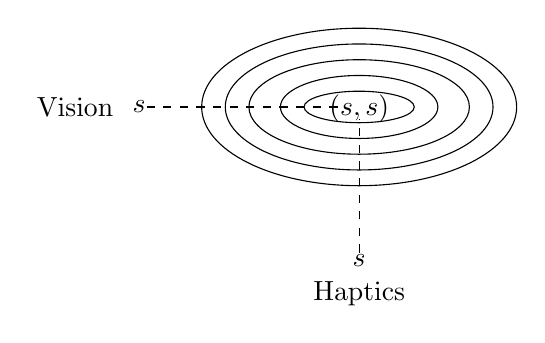
\begin{tikzpicture}
\draw (3,2.15) ellipse (2cm and 1cm);
\draw (3,2.15) ellipse (1.7cm and 0.8cm);
\draw (3,2.15) ellipse (1.4cm and 0.6cm);
\draw (3,2.15) ellipse (1cm and 0.4cm);
\draw (3,2.15) ellipse (0.7cm and 0.2cm);
\node [above] at (3, 1.825) {$(s,s)$};
\node [right] at (0, 2.15) {$s$};
\node [left] at (0, 2.15) {Vision};
\node [above] at (3, 0) {$s$};
\node [above] at (3, -0.5) {Haptics};
\draw [dashed] (0.3, 2.15) -- (2.8, 2.15);
\draw [dashed] (3, 0.3) -- (3, 2);
\end{tikzpicture}
\end{figure}

Given the length of the bar ($s$) this is the probability for our haptic ($h$) and visual ($v$) impression:
\smallskip
\begin{align*}
p\left(V=v;H=h|s\right)=\frac{1}{\sqrt{2\pi}\sigma_{V}}e^{-\frac{1}{2}\left(\frac{v-s}{\sigma_{V}}\right)^{2}}\frac{1}{\sqrt{2\pi}\sigma_{H}}e^{-\frac{1}{2}\left(\frac{h-s}{\sigma_{H}}\right)^{2}}
\end{align*}

Together with the log-likelihood we can calculate a ML-Estimate $\hat{s}$ for $s$:
\begin{align*}
\Rightarrow -\frac{1}{2}\left(\left(\frac{v-\hat{s}}{\sigma_{V}}\right)^{2} + \left(\frac{h-\hat{s}}{\sigma_{H}}\right)^{2}\right) = -\frac{1}{2}\left(\frac{v-\hat{s}}{\sigma_{V}}\right)^{2} -\frac{1}{2} \left(\frac{h-\hat{s}}{\sigma_{H}}\right)^{2}
\end{align*}
Use first derivative:

\begin{align*}
& & \left(\frac{v-\hat{s}}{\sigma_{V}}\right) \frac{2}{2\sigma_{V}} + \left(\frac{h-\hat{s}}{\sigma_{H}}\right) \frac{2}{2\sigma_{H}} & \stackrel{!}{=}0 & & \\
\Leftrightarrow & & \frac{v-\hat{s}}{\sigma_{V}^{2}} + \frac{h-\hat{s}}{\sigma_{H}^{2}} & = 0 & & \\
\Leftrightarrow & & \frac{v}{\sigma_{V}^{2}} + \frac{h}{\sigma_{H}^{2}} -\hat{s} \left(\frac{1}{\sigma_{V}^{2}} + \frac{1}{\sigma_{H}^{2}}\right) & = 0 & & \\
\Leftrightarrow & & \frac{v}{\sigma_{V}^{2}} + \frac{h}{\sigma_{H}^{2}} & = \hat{s} \left(\frac{1}{\sigma_{V}^{2}} + \frac{1}{\sigma_{H}^{2}}\right) & & \\
\Leftrightarrow & & \hat{s} & = \left(\frac{v}{\sigma_{V}^{2}} + \frac{h}{\sigma_{H}^{2}}\right) \frac{\sigma_{V}^{2}\sigma_{H}^{2}}{\sigma_{V}^{2} + \sigma_{H}^{2}} & & \\
\Leftrightarrow & & \hat{s} & = \frac{v\sigma_{H}^{2}}{\sigma_{V}^{2} + \sigma_{H}^{2}} + \frac{h\sigma_{V}^{2}}{\sigma_{V}^{2} + \sigma_{H}^{2}} & &
\end{align*}

This estimate seems logical, since the variances are used as a normalization term in the denominator and the numerator weights our sensation according to their internal variance. In our example we assumed the visual system to have a small variance compared to the haptic system, so the $v$ has greater impact on $\hat{s}$.

\end{document}


%\clearpage

% Practice: Signal Detection Theory III
\iftoggle{exercises}{
  %\includepdf[pages={-},
      %addtotoc={1,section,1,Tutorial Sheet ,exsheet},
      %viewport=100 50 550 700,
      %scale=0.75,
      %pagecommand=\thispagestyle{plain}
      %]{exercises/Exercises0.pdf}
}{}
\iftoggle{solutions}{
%  \documentclass[../main/Notes.tex]{subfiles}
\begin{document}

\section[Solution 7: Signal Detection Theory III]{Solution 7: Signal Detection Theory III \iftoggle{showdates}{\small{\textit{2014-06-30}}}{}}

\subsection*{Exercise 1}\index{Poisson Distribution}
Why do we always use a Gaussian to model all those things? Can't we just use other models as well? 

We think about neurons as Poisson processes.

If we just look at the spikes, a neuron's firing behavior looks roughly like figure \ref{fig:2014-06-30_firing_neuron_data}. To model it, we discretize over time and say for each cell whether the neuron fires or not (figure \ref{fig:2014-06-30_firing_neuron_model}) and can then calculate the probability.

\begin{figure}[htb]
  \centering
  \begin{subfigure}{.45\textwidth}
    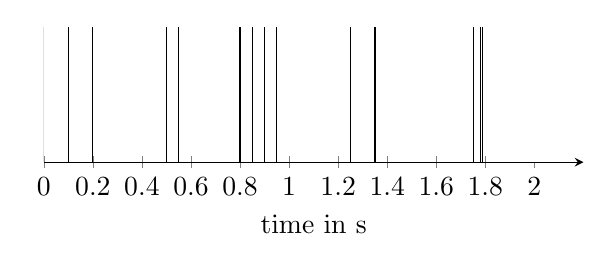
\begin{tikzpicture}
      \begin{axis}[domain=0:2, ymin=0, ymax=0.1, no markers, xtick={0,0.2,0.4,0.6,0.8,1.0,1.2,1.4,1.6,1.8,2.0}, axis x line=bottom, axis y line=none, enlargelimits=upper, y post scale=0.3, xlabel={time in s}]
        \foreach \x in {0,0.1,0.2,0.5,0.55,0.8,0.85,0.9,0.95,1.25,1.35,1.75,1.78,1.79}
          \addplot[black] coordinates{(\x,0) (\x,1)};
        \addplot[white] coordinates{(2,0) (2,1)};
      \end{axis}
    \end{tikzpicture}
    \caption{``Data'' for firing neurons: each line stands for a firing.}
    \label{fig:2014-06-30_firing_neuron_data}
  \end{subfigure}
  \begin{subfigure}{.45\textwidth}
    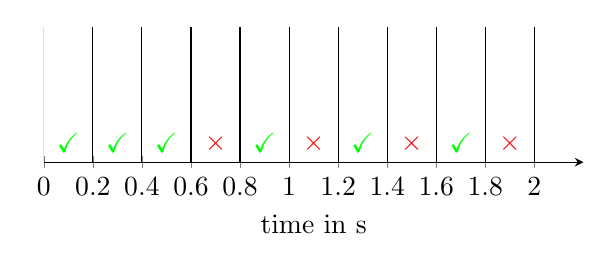
\begin{tikzpicture}
      \begin{axis}[domain=0:2, ymin=0, ymax=0.1, no markers, xtick={0,0.2,0.4,0.6,0.8,1.0,1.2,1.4,1.6,1.8,2.0}, axis x line=bottom,axis y line=none, enlargelimits=upper, y post scale=0.3, xlabel={time in s}]
        \foreach \x in {0,0.2,0.4,0.6,0.8,1.0,1.2,1.4,1.6,1.8,2.0}
          \addplot[black] coordinates{(\x,0) (\x,1)};
        \node[above,green] at (axis cs:0.1,0) {$\checkmark$};
        \node[above,green] at (axis cs:0.3,0) {$\checkmark$};
        \node[above,green] at (axis cs:0.5,0) {$\checkmark$};
        \node[above,red]   at (axis cs:0.7,0) {$\times$};
        \node[above,green] at (axis cs:0.9,0) {$\checkmark$};
        \node[above,red]   at (axis cs:1.1,0) {$\times$};
        \node[above,green] at (axis cs:1.3,0) {$\checkmark$};
        \node[above,red]   at (axis cs:1.5,0) {$\times$};
        \node[above,green] at (axis cs:1.7,0) {$\checkmark$};
        \node[above,red]   at (axis cs:1.9,0) {$\times$};
      \end{axis}
    \end{tikzpicture}
    \caption{Model for firing neurons: Bins to show whether a neuron fired during that time or not.}
    \label{fig:2014-06-30_firing_neuron_model}
  \end{subfigure}
  \caption{Example data for firing neurons and the respective model}
  \label{fig:2014-06-30_firing_neurons}
\end{figure}

We can then find the distribution over time for the neuron by taking an interval of time and counting the number of spikes. This will result in the Poisson distribution: $P(N=n|r,t)=\frac{(rt)^n}{n!}e^{rt}$.

Assuming we have 10 spikes in a second and plug this into the Poisson distribution, we should intuitively end up with 10 Hz.

\begin{align*}\index{Maximum likelihood}
P(N=n|r,t) &= \frac{(rt)^n}{n!} e^{-rt} \\
\log{P(N=n|r,t)} &= n \log{rt} - \log{n!} - rt \\
\frac{\partial\log{P(N=n|r,t)}}{\partial r} &= \frac{n}{rt}t-t \\
\frac{\partial^2\log{P(N=n|r,t)}}{\partial^2 r} &= \frac{n}{r^2} \\
\text{Use the first derivative to maximize it:}\\
\frac{n}{\est{r}t}t-t &= 1 \\
\frac{n}{\est{r}t} &= 1 \\
\frac{n}{t} &= \est{r}
\end{align*}

\subsubsection*{Bonus Question}
\begin{align*}
E(N) &= \sum_{n=0}^\infty{n \frac{(rt)^n}{n!} e^{-rt}} \\
     &= e^{-rt} \sum_{n=0}^\infty{\frac{(rt)^n}{(n-1)!}} \\
\text{use:}&\\
\sum_{n=0}^\infty{\frac{(rt)^n}{n!} e^{-rt}} &= 1 \\
\text{for:}&\\
E(N) &= e^{-rt} (rt) \sum_{n=1}^\infty{\frac{(rt)^{(n-1)}}{(n-1)!}} \\
     &= e^{-rt} (rt) \sum_{n=0}^\infty{\frac{(rt)^{n}}{n!}} \\
     &= e^{-rt} (rt) e^{rt} = rt
\end{align*}
So it's exactly what we said above: If we have 10 spikes in a second, we come up with 10 Hz.
\begin{align*}
var(N) &= E(N^2)-E(N)^2 \\
       &= \sum_{n=0}^\infty{n^2 \frac{(rt)^n}{n!} e^{-rt}} - (rt)^2 \\
       &= \sum_{n=0}^\infty{(n+1) \frac{(rt)^{n+1}}{n!} e^{-rt}} \\
       &= (rt)e^{-rt}\left[ \underbrace{ \sum_{n=0}^\infty{n \frac{(rt)^n}{n!}} }_{rt\cdot e^{rt}} +  \underbrace{ \sum_{n=0}^\infty{\frac{(rt)^n}{n!}} }_{e^{rt}} \right] - (rt)^2 \\
       &= (rt)e^{-rt}\left(rt e^{rt}+e^{rt}\right) - (rt)^2 \\
       &= (rt)(rt+1)-(rt)^2 = rt
\end{align*}
This variance corresponds with the Weber-Fechner-law (for details see \href{http://en.wikipedia.org/wiki/Weber-Fechner_law}{Wikipedia}): If the signal increases, also the noise (i.e. the variance) increases.

\subsection*{Exercise 2}
% distribution here
\begin{align*}
\frac{P(N=n|r=80 Hz, t = 100 ms)}{P(N=n|r=20 Hz, t = 100 ms)} &= \frac{ \frac{8^n}{n!}e^{-8} }{ \frac{2^n}{n!} e^{-2} } = \left(\frac{8}{2}\right)^n e^{-8+2}
\end{align*}

For the intersection we set $\left(\frac{8}{2}\right)^n e^{-8+2} = 1$.
\begin{align*}
\left(\frac{8}{2}\right)^n e^{-8+2} &= 1\\
4^n &= e^6 \\
n \log 4 &= 6 \\
n &\approx 4.3
\end{align*}

\subsection*{Exercise 3}


\subsection*{Exercise 4}


\subsection*{Exercise 5}


\end{document}

%  \clearpage
}{}

% Choice Models I
%\documentclass[../main/Notes.tex]{subfiles}
\begin{document}

\section[Solution 6: Signal Detection Theory xxxBut which number to put here?xxx]{Solution 6: Signal Detection Theory I+II \iftoggle{showdates}{\small{\textit{2014-06-27}}}{}}

\subsection*{Excercise 4}\index{Low Threshold Theory}\label{sheet6ex4}

Luce's idea is: If High Threshold Theory does not work, maybe by using a low threshold, ROC curves will be explainable. This idea translates as follows:

\begin{align*}
S \in \{ y,n \} , D \in \{ y,n \} , R \in \{ y,n \} \\
P\left(D=y|S=y\right) = p_{y} \\
P\left(D=y|S=n\right) = p_{n} > 0
\end{align*}

We have to consider to different cases of the subject's behaviour.

\textbf{Case 1:} The subject want to lower his false-alarm rate $p(FA)$:
\begin{align*}
& P\left(R=y|D=n\right) = 0 \\
& P\left(R=y|D=y\right) = t < 1\\
\Rightarrow P(FA) & = P\left(R=y|D=y\right) &\cdot~& P\left(D=y|S=n\right) &+~&P\left(R=y|D=n\right)&\cdot~ & P\left(D=n|S=n\right) \\
& = t &\cdot~& p_{n} &+~& 0 &\cdot~& \left(1-p_{n}\right) \\
& = t \cdot~ p_{n} \\
\Rightarrow P(H) & = P\left(R=y|D=y\right) &\cdot~& P\left(D=y|S=y\right) &+~&P\left(R=y|D=n\right)&\cdot~ & P\left(D=n|S=y\right) \\
& = t &\cdot~& p_{y} &+~& 0 &\cdot~& \left(1-p_{y}\right) \\
& = t \cdot~ p_{y} \\
& = \frac{P(FA)}{p_{n}} \cdot~ p_{y}
\end{align*}

Now the first part of the plot looks like this:
\begin{figure}[ht!]
  \centering
  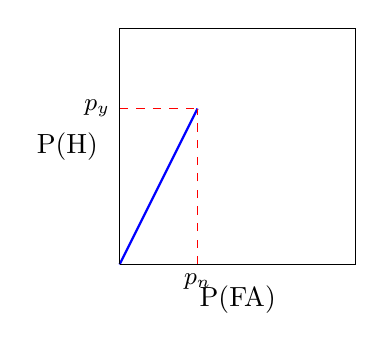
\begin{tikzpicture}[scale=3]
  \node[below] at (0.33,0) {\small $p_{n}$};
  \node[left] at (0,0.66) {\small $p_{y}$};
    \node[below] at (0.5,-0.05) {P(FA)};
  \node[left] at (-0.05,0.5) {P(H)};
  \draw[thick, blue] (0,0) -- (0.33,0.66);
  \draw[dashed, red] (0.33,0) -- (0.33,0.66);
   \draw[dashed, red] (0,0.66) -- (0.33,0.66);
   	\draw (0,0) -- (0,1) --(1,1) -- (1,0) -- (0,0);
  \end{tikzpicture}
  \caption{Low Threshold Model, first part of plot with slope of $\frac{p_{y}}{p_{n}}$}
  \label{fig:2014-06-27_firstPartLowThrsh}
\end{figure}

\textbf{Case 2:} The subject wants a higher hit rate $p(H)$:
\begin{align*}
& P\left(R=y|D=Y\right) = 1 \\
& P\left(R=y|D=n\right) = u > 0\\
\Rightarrow P(FA) & = P\left(R=y|D=y\right) &\cdot~& P\left(D=y|S=n\right) &+~&P\left(R=y|D=n\right)&\cdot~ & P\left(D=n|S=n\right) \\
& = 1 &\cdot~& p_{n} &+~& u &\cdot~& \left(1-p_{n}\right) \\
& = p_{n} + u \cdot~ \left(1-p_{n}\right)\\
\Leftrightarrow u &= \frac{P(FA)-p_{n}}{1-p_{n}} \\
\Rightarrow P(H) & = P\left(R=y|D=y\right) &\cdot~& P\left(D=y|S=y\right) &+~&P\left(R=y|D=n\right)&\cdot~ & P\left(D=n|S=y\right) \\
& = 1 &\cdot~& p_{y} &+~& u &\cdot~& \left(1-p_{y}\right) \\
& = p_{y} +  u \cdot~  \left(1-p_{y}\right)\\
& = p_{y} +  \frac{P(FA)-p_{n}}{1-p_{n}} \cdot~  \left( 1-p_{y} \right)\\
& = \frac{1-p_{y}}{1-p_{n}} \cdot~ P(FA) + \frac{p_{y}-p_{n}}{1-p_{n}}
\end{align*}

We can finish our plot:
\begin{figure}[ht!]
  \centering
  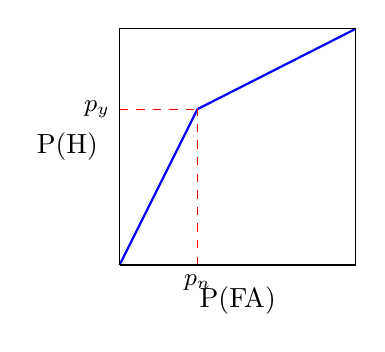
\begin{tikzpicture}[scale=3]
  \node[below] at (0.33,0) {\small $p_{n}$};
  \node[left] at (0,0.66) {\small $p_{y}$};
    \node[below] at (0.5,-0.05) {P(FA)};
  \node[left] at (-0.05,0.5) {P(H)};
  \draw[thick, blue] (0,0) -- (0.33,0.66);
   \draw[thick, blue] (0.33,0.66) -- (1,1);
  \draw[dashed, red] (0.33,0) -- (0.33,0.66);
   \draw[dashed, red] (0,0.66) -- (0.33,0.66);
   	\draw (0,0) -- (0,1) --(1,1) -- (1,0) -- (0,0);
  \end{tikzpicture}
  \caption{Low Threshold Model Plot}
  \label{fig:2014-06-27_LowThrshPlot}
\end{figure}

As can be seen, Low Threshold Theory better fits the actual data since its form is, compared with the linear function of High Threshold Theory, more like that of an ROC curve. Nevertheless it is not the right model for what is really going on.

\end{document}
%\clearpage

% Practice: Choice Models I
\iftoggle{exercises}{
  %\includepdf[pages={-},
      %addtotoc={1,section,1,Tutorial Sheet ,exsheet},
      %viewport=100 50 550 700,
      %scale=0.75,
      %pagecommand=\thispagestyle{plain}
      %]{exercises/Exercises0.pdf}
}{}
\iftoggle{solutions}{
%  \documentclass[../main/Notes.tex]{subfiles}
\begin{document}

\section[Choice Models II]{Choice Models II \iftoggle{showdates}{\small{\textit{2014-07-07}}}{}}\index{Choice models}

\subsection{Thurstone Scaling}\index{Thurstone Scaling}
In 1920 Thurstone thought about measurements in Psychology. He conducted an experiment where he asked the subjects whether they think that one crime is more serious than another. Of course there exists no thing like a crime-seriousness scale, but by comparing all pairs of answers, Thurstone could construct one.

\bigskip
This technique is also used in the Elo rating (famous amongst chess players) or the similar X-Box's Trueskill. These scales are used to match players of equal skill. The problem is, that you lack enough data to apply our method (you will never have a nearly complete matrix of all X-Box players competing against each other in one specific game). Good thing: we do not need the whole matrix! For subsets of the matrix we can predict new matches based on common past enemies. And (considering the X-Box setting) the matchmake can also optimize their information by matching the right people together. But how do we know, that all this rating is formally correct?

\subsection{A little bit of Measurement Theory} 
Consider the problems of an IQ-Test. You lack a concrete scale for the intelligence of a person as well as a 'suitable' opponent for a match up. The solution: to match the subject against the test items.

\begin{figure}[htb]
  \centering
  \begin{tikzpicture}
    \begin{axis}[enlargelimits=false,domain=0:11, mark=none, axis x line*=bottom, axis y line*=left, xlabel ={IQ}]
      \addplot[red, samples=100]   {gauss(3,1)};
        \addlegendentry{$Subject_1$}
      \addplot[green, samples=100] {gauss(1.5,1)};
        \addlegendentry{$Subject_2$}
      \addplot[blue, samples=100]  {gauss(6,1)};
        \addlegendentry{$Subject_3$}
      \foreach \x in {1.25,2.9,8,6.5}
          \addplot[black] coordinates{(\x,0) (\x,0.4)};
    \end{axis}
  \end{tikzpicture}
  \caption{Performance of 3 subjects in an IQ-Test.}
  \label{fig:2014-07-07-iqTest}
\end{figure}
The test items mark thresholds similar to signal detection theory: you answer a question correctly and you are right of it, you fail you are left. Now it is possible to calculate simultaneously the position of the thresholds on the IQ-scale, as well as the IQ-scale itself (we do not discuss how to do this in detail). 

\subsubsection{What are the underlying assumptions of our "`Measurement Model"'?}
Obviously we assume some kind of ordering between the different items. There is a fancy word for this:

\subsubsection{Weak Stochastic Transitivity}\index{Weak Stochastic Transitivity}
If $\mu_i \geq \mu_j,\mu_j \geq \mu_k$ then $\mu_i \geq \mu_k$. In this case transitivity holds. We can rewrite this:
\begin{align*}
&\underbrace{\mu_i-\mu_j \geq 0}_{d_{ij}},\underbrace{\mu_j-\mu_k \geq 0}_{d_{jk}} \Rightarrow \underbrace{\mu_i-\mu_k \geq 0}_{d_{ik}}\\
&\Leftrightarrow p_{ij} \geq \frac{1}{2}, p_{jk} \geq \frac{1}{2} \Rightarrow p_{ik} \geq \frac{1}{2}
\end{align*}
So weak stochastic transitivity is about ordering of the different choices, but is less restrictive about the values. This constraint is exploited by:

\subsubsection{Strong Stochastic Transitivity}\index{Strong Stochastic Transitivity}
If we know that choice $i$ is preferred over choice $j$ and $j$ is chosen over $k$, the resulting choice probability of $i$ over $k$ can not be less, than the maximum of the single probabilities:
\begin{align*}
d_{ij} \geq 0, d_{jk} \geq 0 &\Rightarrow d_{ik} = d_{ij}+d_{jk} \geq max(d_{ij},d_{jk})\\
p_{ij} \geq \frac{1}{2}, p_{jk} \geq \frac{1}{2} &\Rightarrow p_{ik} \geq max(p_{ij},p_{jk})
\end{align*}
Strong stochastic transitivity may be violated in the case where the variances of the different choices differ:
\begin{figure}[htb]
  \centering
  \begin{tikzpicture}
    \begin{axis}[enlargelimits=false,domain=0:13, mark=none, axis x line*=bottom, axis y line*=left, xlabel ={IQ}]
      \addplot[red, samples=100]   {gauss(1,1)};
        \addlegendentry{$k$}
      \addplot[green, samples=100] {gauss(5.5,1)};
        \addlegendentry{$j$}
      \addplot[blue, samples=100]  {gauss(8,3)};
        \addlegendentry{$i$}
      \end{axis}
  \end{tikzpicture}
  \caption{A problem for strong stochastic probability}
  \label{fig:2014-07-07-strongStochTrans}
\end{figure}

In this case $p_{ij} = 0.6$, $p_{jk}=0.95$ but $p_{ik} = 0.85$ which is less than the maximum of the other probabilities $0.95$! But we can also think of different examples where the whole concept of transitivity is questionable.

\subsubsection{Is transitivity reasonable?}
Assume a situation of three chess players $A, B,$ and $C$. $A$ more often beats $B$ than losing against him, $B$ more often beats $C$ but $C$ also more often beats $A$ than losing against her. This scenario is visualized in figure \ref{fig:2014-07-04-chesscycle}. If we try to find Gaussian distributions for each player's utility it gets clear quite quickly, that we will fail, since we don't know ``where'' to put the $\mu$ for the last competitor: left or right of the other two?

\begin{figure}[ht]
  \centering
  \begin{tikzpicture}
    \node[state] (A) {$A$};
    \node[state] (B) [right=1.5cm of A] {$B$};
    \node[state] (C) [below right=.5cm and .65cm of A] {$C$};
    \path (A) edge [bend left,->] node {} (B)
          (B) edge [bend left,->] node {} (C)
          (C) edge [bend left,->] node {} (A);
  \end{tikzpicture}
  \caption{Three chessplayers dominate each other in a cyclic way.}
  \label{fig:2014-07-04-chesscycle}
\end{figure}

It seems our measurement model is not appropriate for this kind of situation. But how can we decide whether our model is appropriate or not?

\subsubsection{Restle's Choice Model}
Another model that does not assume one dimensional scaling for choices was proposed by Restle. In 1961 he showed with a gedankenexperiment why our previous model is maybe not that accurate and intuitive as it first sounded. Consider the following setting: we would like to go on holiday and have the following alternatives:
\begin{itemize}
  \item Rome
	\item Paris
  \item Paris + an apple
\end{itemize}
If we are indifferent between Paris and Rome ($p_{21} = p_{12} = \frac{1}{2}$) -- what is $p_{32}$? Actually the one extra apple should not change our basic decision between Paris and Rome, so $p_{32} \approx \frac{1}{2}$, but strong stochastic transitivity would predict $p_{32} = 1$! So if our previous model would be right every travel agent could simply persuade you to book any vacation by simply having an apple at hand.

Restle proposes a binary feature vector that describes each option. Ours look like $(Paris, Rome, Apple)$:
\begin{align*}
f_1 = (0, 1, 0)\\
f_2 = (1, 0, 0)\\
f_3 = (1, 0, 1)
\end{align*}
Each feature has a utility $\mu_1,\mu_2,\mu_3$ and the probability to choose one over the other $i$s dependent on the sum of all the features one choice has compared to the other. In the following formula $m$ is the dimension of the feature vector.
\begin{align*}
p_{ij} &\propto \sum_{k=1}^{m}\mu_k(f_{ik}-f_{ik}\cdot f_{jk}) = u_{ij}\\
p_{ij} &= \frac{u_{ij}}{u_{ij}+u_{ji}}
\end{align*}
Let's calculate the probability with which we choose Rome over Paris:
\begin{align*}
p_{12} &= \frac{\sum_{k=1}^3\mu_k(f_{1k}-f_{1k} \cdot f_{2k})}{u_{12}+u_{21}}\\
       &= \frac{\mu_2}{\mu_2+\mu_1} = \frac{1}{2} \text{ , if $\mu_1=\mu_2$}
\end{align*}
Now we calculate the interesting choice Paris+Apple over Rome:
\begin{align*}
p_{31} &= \frac{\sum_{k=1}^3\mu_k(f_{1k}-f_{1k} \cdot f_{2k})}{u_{31}+u_{13}}\\
       &= \frac{\mu_1+\mu_3}{\mu_1+\mu_3+\mu_2} \approx \frac{1}{2} \text{ , since $\mu_3 << \mu_2$}
\end{align*}
So Restle's model can predict this scenario much better.
\end{document}

%  \clearpage
}{}

% Choice Models II
%\documentclass[../main/Notes.tex]{subfiles}
\begin{document}

\section[Choice Models I]{Choice Models I\iftoggle{showdates}{\small{\textit{2014-07-04}}}{}}\index{Choice models}

\subsection*{Utility}\index{Utility}
\begin{wrapfigure}{r}{.3\textwidth}
   \centering
  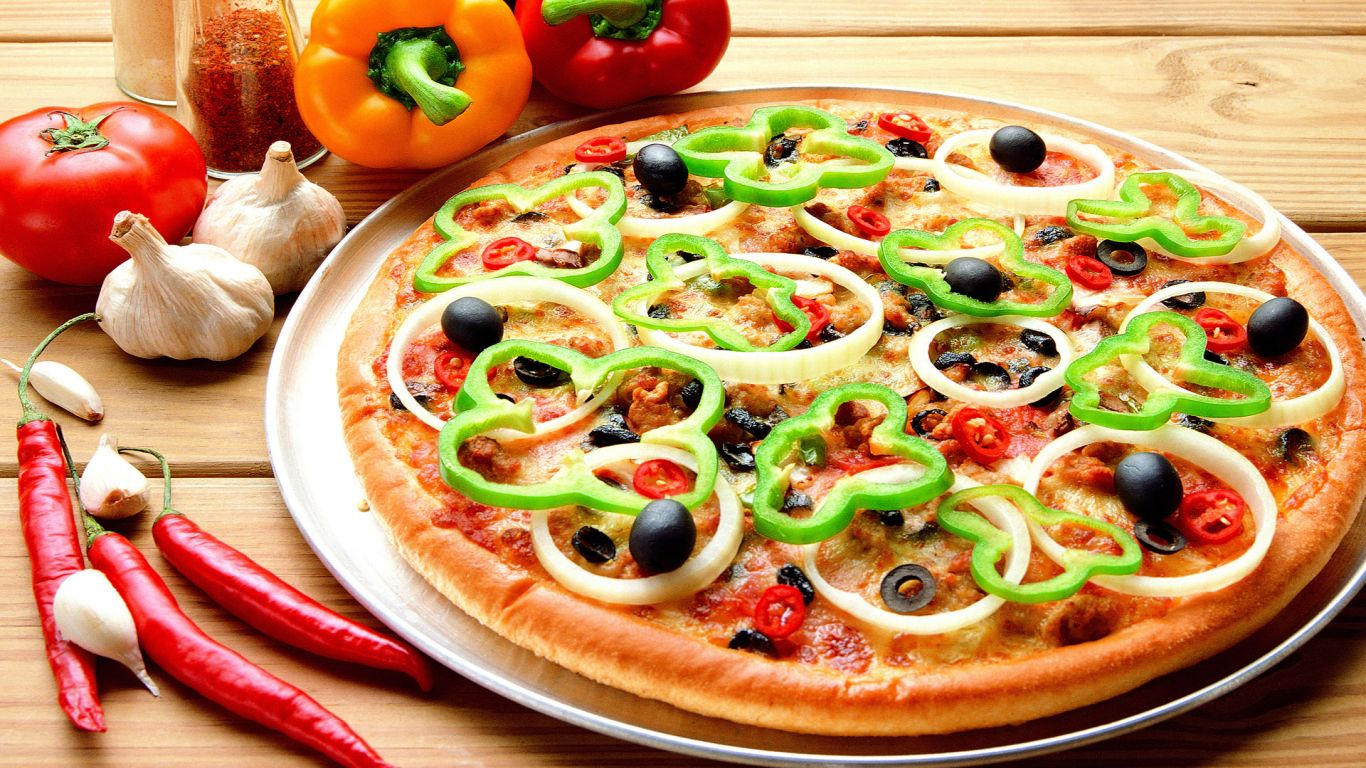
\includegraphics[width=.3\textwidth]{../images/pizza-free-wallpaper_1366x768_82178.jpg}
  \caption{Pizzaaaa!}
  \label{fig:2014-07-04-pizza}
\end{wrapfigure}
The \emph{utility} is the variability in choices. It can either refer to the variability in choices of several subjects (``How many subjects prefer pizza tonno over pizza salami?'') or the variability in choices of a single subject over time (``On how many days prefers the subject pizza tonno over pizza salami?''). A utility of e.g. 70\% means that a subject chooses pizza tonno over pizza salami in 70 out of 100 times it's asked.

With choice models we try to find the utility of possible choices in order to make accurate predictions.

Note that there might be \emph{polarizing} options, this means the variance changes. For example pizza margarita might be very popular, so many people like it thus the variance for a choice of pizza margarita gets smaller. However, pizza salami might be less popular and therefor its utility's variance is wider (see figure \ref{fig:2014-07-04-polarizing}.

Since the utility is dependent on the choice to made, there can only be \emph{relative} utilities.
\begin{figure}
\centering
\begin{tikzpicture}
  \begin{axis}[every axis plot post/.append style={mark=none, domain=-2:8, samples=50, smooth}, 
    axis x line*=bottom, axis y line*=left, enlargelimits=upper,yticklabels={},xticklabels={}]
    \addplot [red]    {gauss(0,0.5)};
      \addlegendentry{Pizza Margarita}
    \addplot [green]  {gauss(4,2)};
      \addlegendentry{Pizza Salami}
  \end{axis}
\end{tikzpicture}
\caption{Red: Pizza margarita is quite popular among all subjects. Green: Pizza salami is not that popular among subjects, it has a higher variance.}
\label{fig:2014-07-04-polarizing}
\end{figure}

\subsection{Paired Comparison Experiment}\index{Paired Comparison Experiment}
A very common technique to check whether subjects prefer an option over another is a paired comparison experiment. Subjects are shown \emph{all possible pairs} and say for each pair which option they prefer. This results in a matrix where we can find out which options are more popular than others. See table \ref{tab:2014-07-04-example_paired_comp_exp} for an example.

% todo: make this table more beautiful
\begin{table}
\centering
\begin{tabular}{l|c|c|c|}
\multicolumn{1}{l}{\rotatebox{45}{are chosen}} & \multicolumn{3}{c}{over these options} \\ \cline{2-4}\rule[-2.5ex]{0pt}{7ex}
\multirow{3}{1em}{\rotatebox{90}{these options}} & --- & $\frac{15}{60}$ & $\frac{40}{60}$ \\ \cline{2-4}\rule[-2.5ex]{0pt}{7ex}
& $\frac{45}{60}$ & --- & $\frac{30}{60}$ \\  \cline{2-4}\rule[-2.5ex]{0pt}{7ex}
& $\frac{20}{60}$ & $\frac{30}{60}$ & --- \\ \cline{2-4}
\end{tabular}
\caption{Example paired comparison outcome. In this example we assume we asked 60 subjects, hence the denominator.\\For computations we often set the diagonal (compare each option with itself) to $\frac{1}{2}$, which means there is no preference -- this already makes sense intuitively.}
\label{tab:2014-07-04-example_paired_comp_exp}
\end{table}

\subsubsection*{Two options}
\sidenote{To make it easier to understand the math we will assume equal variance for given options unless noted otherwise.}
Assume we ask a subject to make a choice between two options. We consider two options $i$ and $j$ with the random variables $x_i$ and $x_j$ as their utilities (the subject's utilities for each option respectively) with $x_i \sim \mathcal{N}\left(\mu_i,1\right)$ and $x_j \sim \mathcal{N}\left(\mu_j,1\right)$. The subject ``computes'' $\Delta x_{ij} = x_i - x_j$ if $\Delta x_{ij} > 0$ (otherwise we would need $\Delta x_{ji}$). $\Delta x_{ij}$ is also normal distributed, i.e. $\Delta_x{ij} \sim \mathcal{N}\left(\mu_i-\mu_j,2\right)$. $\Delta x_{ij}$ is the distribution of how likely it is, that the subject chooses $i$ over $j$. A visualization of this can be found in figure \ref{fig:2014-07-04-compute_delta_xij}.

\begin{figure}
\centering
\begin{tikzpicture}
	\begin{axis}[domain=-2:6, enlargelimits=upper, axis x line*=bottom, axis y line*=left]
    \addplot [red,samples=50]   {gauss(1,1)};
      \addlegendentry{$x_j$};
    \addplot [green,samples=50] {gauss(3,1)};
      \addlegendentry{$x_i$};
    \addplot [blue,samples=50]  {gauss(2,2)};
      \addlegendentry{$\Delta x_{ij}$};
  \end{axis}
\end{tikzpicture}
\begin{tikzpicture}
  \begin{axis}[domain=-2:8, enlargelimits=upper, axis x line*=bottom, axis y line*=left]
    \addplot [red,samples=50]   {gauss(1,0.75)};
      \addlegendentry{$x_j$};
    \addplot [green,samples=50] {gauss(4,1.5)};
      \addlegendentry{$x_i$};
    \addplot [blue,samples=50]  {gauss(3,2.25)};
      \addlegendentry{$\Delta x_{ij}$};
  \end{axis}
\end{tikzpicture}
\caption{Relation of $x_i, x_j$ and $\Delta x_{ij}$. Left: two options with equal variance. Right: two options with different variances. Note that the variances add up, hence $\Delta x_{ij}$ gets flat and wide.}
\label{fig:2014-07-04-compute_delta_xij}
\end{figure}

\begin{figure}
  \centering
  \begin{tikzpicture}
    \begin{axis}[domain=-5:2, enlargelimits=upper, axis x line*=bottom, axis y line*=left]
      \addplot+[domain=0:2, samples=100, pattern=flexible hatch, mark=none
                hatch distance=5pt, hatch thickness=0.5pt,
                draw=green, pattern color=green!40, area legend]
                {gauss(-3,2)} \closedcycle;
        \addlegendentry{$\int\limits_0^\infty\Delta x_{ij}$}
      \addplot[domain=-5:2, samples=50, red] {gauss(-3,2)};
        \addlegendentry{$\Delta x_{ij}$}
      \draw[-,below] (axis cs:0,0)--(axis cs:0,1) node{0};
      \draw[-,dashed,above] (axis cs:0.5,0.025)--(axis cs:1,0.1) node{$\mathcal{A}$};
      \draw[-,dotted,above] (axis cs:-3,-0.01)--(axis cs:-3,0.2) node{$\mu_i-\mu_j$};
    \end{axis}
  \end{tikzpicture}
  \caption{$\Delta x_{ij}$: If we know this area $\mathcal{A}$, we can guess $\Delta \mu_{ij}$.}
  \label{fig:2014-07-04-guessing_delta_mu}
\end{figure}

\subsubsection*{Definitions}
We define:
\begin{itemize}
	\item $d_{ij} = \mu_i-\mu_j$
  \item $p_{ij}$ is the probability that the subject chooses $i$ over $j$.
  \item $P_{ij} = 1-P_{ji} = 1-\Phi(d_{ij};0,\sqrt{2}) = 1-\Phi(-d_{ij};0,\sqrt{2}) \stackrel{\text{\footnotesize z-tf.}}{=} 1-\Phi\left(-\frac{d_{ij}}{\sqrt{2}};0,1\right)$
     \\ Figure \ref{fig:2014-07-04-Phi0} shows visually that $\Phi(x)=1-\Phi(-x)$, so we can write $1-\Phi\left(-\frac{d_{ij}}{\sqrt{2}};0,1\right) = \Phi\left(\frac{d_{ij}}{\sqrt{2}};0,1\right)$.
     \\ To further simplify the notation we just write $\Phi\left(\frac{d_{ij}}{\sqrt{2}}\right)$.
  \item $q_{ij}$
\end{itemize}

\begin{figure}
  \centering
  \begin{tikzpicture}
    \begin{axis}[restrict x to domain=-2:2, restrict y to domain=0:1.1, enlargelimits=false, axis x line*=bottom, axis y line*=left, legend style={at={(1,0.5)},anchor=east}]
      \addplot[mark=none,red,samples=50,domain=-2:2]{Gauss(0,1)};
        \addlegendentry{$\Phi(x)$}
      \addplot[mark=none,blue,samples=50,domain=-2:2]{(1/(1+exp(-0.07056*(-x)^3-1.5976*(-x)))};
        \addlegendentry{$\Phi(-x)$}
    \end{axis}
  \end{tikzpicture}
  \caption{$\Phi(x)=1-\Phi(-x)$}
  \label{fig:2014-07-04-Phi0}
\end{figure}

\subsection*{Optimizing Paired Comparison Experiment}
We search for an estimate of $d_{ij}$. We can use $q_{ij} = \Phi\left(\frac{\est{d_{ij}}}{\sqrt{2}}\right)$ and derive $\Phi^-1\left(q_{ij}\right) = \frac{\est{d_{ij}}}{\sqrt{2}} \Leftrightarrow \sqrt{2}\Phi^{-1}\left(q_{ij}\right) = \est{d_{ij}}$.

\sidenote{$\forall i\!: \est{d_{ii}}=0$}
$\est{d}$ is a matrix (figure \ref{fig:2014-07-04-est_d_exp}) with the estimated distances for $\est{d_{ij}} = \est{\mu_i}-\est{\mu_j}$. Hence $\est{d_{ij}}=-\est{d_{ji}}$. But what are good estimates for $\est{\mu_i}$ and $\est{\mu_j$}?

\begin{figure}[hb]
  \centering
  \begin{align*}
    \est{d}=\left( \begin{array}{ccccc}
      0            &   & \cdots & \est{d_{ij}} &  \\
                   & 0 &        &              &  \\
      \vdots       &   & 0      &              & \vdots \\
      \est{d_{ji}} &   &        & 0            &  \\
                   &   & \cdots &              & 0 
    \end{array} \right)
  \end{align*}
  \caption{$\est{d}$, note that $d_{ji} = -d_{ij}$ and the diagonal is 0.}
  \label{fig:2014-07-04-est_d_exp}
\end{figure}

We have $\frac{n(n-1)}{2}$ pairs, that means we have $(n-1)$ free parameters. This means we will not be able to determine the x-shift. This shouldn't bother us too much, since we are only interested in the difference between $\mu_i$ and $\mu_j$ anyway.

A method for minimizing (thus optimizing) the error in our estimates we can use the least squares estimate (LSE)\index{Least Squares Estimate}.

\subsection{Least Squares Estimate}\index{Least Squares Estimate}
The idea of the least squares estimate is to \emph{minimize the sum of all squared differences}.
\begin{align*}
Q = \frac{1}{2}\left( \sum\limits_j \sum\limits_i \left( \est{\mu_i}-\est{\mu_j} - \est{d_{ij}} \right) \right)
\end{align*}
So we want to minimize $Q$ with respect to $\est{\mu_i}$ and $\est{\mu_j}$. 

This can be done easily by taking the first derivative and setting it to 0.
\begin{align*}
\frac{\partial Q}{\partial \est{\mu_k}} &=             \left( \sum\limits_j \est{\mu_k} - \est{\mu_j} - \est{d_{kj}} \right) - \left( \sum\limits_i \est{\mu_i} - \est{\mu_k}              - \est{d_{ik}} \right) = 0\\
                          &\Leftrightarrow             \left( \sum\limits_j \est{\mu_k} - \est{\mu_j} - \est{d_{kj}} \right) + \left( \sum\limits_i \est{\mu_k} - \est{\mu_i} \underbrace{ + \est{d_{ik}} }_{\text{Remember: }d_{ij}=-d{ji}} \right) = 0\\
                          &\Leftrightarrow \underbrace{\left( \sum\limits_j \est{\mu_k} - \est{\mu_j} - \est{d_{kj}} \right) + \left( \sum\limits_i \est{\mu_k} - \est{\mu_i}              - \est{d_{ki}} \right)}_{\text{twice the same}} = 0\\
                          &\Leftrightarrow           2 \left( \sum\limits_i \est{\mu_k} - \est{\mu_i} - \est{d_{ki}} \right) = 0\\
                          &\Leftrightarrow                    \sum\limits_i \est{\mu_k} - \est{\mu_i} - \est{d_{ki}}         = 0\\
                          &\Leftrightarrow    n \est{\mu_k} -            \sum\limits_i \est{\mu_i} -            \sum\limits_i \est{d_{ki}} = 0 \\
                          &\Leftrightarrow      \est{\mu_k} - \frac{1}{n}\sum\limits_i \est{\mu_i} = \frac{1}{n}\sum\limits_i \est{d_{ki}}
\end{align*}
We end up with $n$ equations (one for each $k$) in $n$ unknowns. However the system's rank is $n-1$, so the system of equations is underdetermined. This means that to solve it we are free to choose something as we want, and obviously we set the average of the $\mu_i$s to 0 and get a nice formula to calculate the average over all distances, $\est{\mu_k}$.
\begin{align*}
\frac{1}{n} \sum\limits_i \est{d_{ki}} \stackrel{!}{=} 0 \Rightarrow \est{\mu_k} = \frac{1}{n} \sum\limits_i \est{d_{ki}}
\end{align*}

\subsubsection*{Simple example}
We have three normal distributions $i, j,$ and $k$ with the means $\mu_i = 1, \mu_j = 0,$ and $\mu_k = -1$ (figure \ref{fig:2014-07-04-normaldists}).
\begin{figure}[htb]
  \centering
  \begin{tikzpicture}
    \begin{axis}[enlargelimits=false, restrict x to domain=-2:2, mark=none, axis x line*=bottom, axis y line*=left]
      \addplot[red, samples=100]   {gauss(1,1)};
        \addlegendentry{$i$}
      \addplot[green, samples=100] {gauss(0,1)};
        \addlegendentry{$j$}
      \addplot[blue, samples=100]  {gauss(-1,1)};
        \addlegendentry{$k$}
    \end{axis}
  \end{tikzpicture}
  \caption{Three normal distributions $i, j,$ and $k$.}
  \label{fig:2014-07-04-normaldists}
\end{figure}

For these distributions we can simply derive the matrix $d$ and calculate the average distance between two plots.

\begin{align*}
d = \left( \begin{array}{ccc}
 0 &  1 & 2 \\
-1 &  0 & 1 \\
-2 & -1 & 0
\end{array} \right)
\end{align*}

\begin{align*}
\mu_i = \frac{1}{n} \sum\limits_l d_{il} = \frac{1}{3} \left( d_{i1} + d_{i2} + d_{i3} \right) = \frac{1}{3} \left( 0 + 1 + 2 \right) = 1
\end{align*}


\end{document}
%\clearpage

% Practice: Choice Models II
\iftoggle{exercises}{
  %\includepdf[pages={-},
      %addtotoc={1,section,1,Tutorial Sheet ,exsheet},
      %viewport=100 50 550 700,
      %scale=0.75,
      %pagecommand=\thispagestyle{plain}
      %]{exercises/Exercises0.pdf}
}{}
\iftoggle{solutions}{
%  \documentclass[../main/Notes.tex]{subfiles}
\begin{document}

\section[Everyday Predictions]{Everyday Predictions \iftoggle{showdates}{\small{\textit{2014-07-14}}}{}}
Galton (1907) went to a fair and observed a simple guessing game. There was a bull displayed and you could get a price if you guessed the right weight of it. Galton had a look at all guesses and found, that the knowledge of the mass could display the real value for the bull's weight (1198 lbs) pretty good as can be seen in the following graph:

\begin{tikzpicture}
\begin{axis}[axis x line*=bottom, axis y line*=left, enlargelimits=upper, axis on top, domain=-4:4, y post scale=0.5, ticks=none ]
%\begin{axis}[every axis plot post/.append style={mark=none, domain=-4:4, samples=50, smooth}, axis x line*=bottom, axis y line*=left, ticks=none, enlargelimits=upper, name=gauss, y post scale=0.5]
  \addplot+[domain=-4:-2.2, samples=100, pattern=flexible hatch, mark=none
            hatch distance=5pt, hatch thickness=0.5pt,
            draw=green, pattern color=green!40, area legend]
            {gauss(0,1)} \closedcycle;
    \addplot+[domain=2.2:4, samples=100, pattern=flexible hatch, mark=none
            hatch distance=5pt, hatch thickness=0.5pt,
            draw=green, pattern color=green!40, area legend]
            {gauss(0,1)} \closedcycle;
    \addplot[color=red, samples=50, smooth] {gauss(0,1)};
    \draw[green] (axis cs: 0,0) -- (axis cs: 0,2);
\end{axis}
\node [above] at (1.35,0.25) {$5\%$};
\node [above] at (5,0.25) {$95\%$};
\node [above] at (1.4,-0.5) {1074};
\node [above] at (4.9,-0.5) {1293};
\node [above] at (3.1,-0.5) {1207};
\node [below] at (3.1,-0.4) {median};
\end{tikzpicture} 

In their paper, Griffiths \& Tenenbaum (2006) did a ``simple'' Bayesian inference with ``real-world'' priors and only one datapoint. An example for this is the distribution of age of death of men in Germany.

\begin{figure}
  \begin{tikzpicture}
    \begin{axis}[axis x line*=bottom, axis y line*=left, enlargelimits=upper, axis on top, domain=0:10, y post scale=0.5, ticks=none]  
      \addplot[color=white, samples=50, smooth, yshift=0.1cm] {gauss(7,1)};
      \addplot[domain=2:10, color=red, samples=50, smooth, yshift=0.1cm] {gauss(7,1)};
      \draw[green] (axis cs: 7.7,0) -- (axis cs:7.7,0.6);
    \end{axis}
    \begin{axis}[axis x line*=bottom, axis y line*=left, enlargelimits=upper, axis on top, domain=0:10, y post scale=0.5, ticks=none, scale=0.2 ]  
      \addplot[color=red, samples=50, smooth, yshift=0.1cm] {gauss(0,1)};
    \end{axis}
    \node [above] at (4.4,-0.5) {80};
    \node [above] at (4.9,-0.5) {85};
    \node [above] at (6,-0.5) {100};
    \node [above] at (3,-0.5) {60};
    \node [above] at (0,-0.5) {0};
  \end{tikzpicture}
  \caption{fig:2014-07-14-deathofmen}
  \label{}
\end{figure}

\bigskip
You meet someone who is 25 years old. When will he die? In this case you have to go with your prior, which then is your posterior.


You meet someone who is 85 years old. When will he die? Every age below 85 is now not possible any more, you have to update your prior.

When X is the total value and Y the observed value, P(X) is our prior. It follows that:
\begin{align*}
& P(Y=y|X=x) & = \frac{1}{X}\cdot I(y\leq x) & & \rightarrow I~is~1~if~y\leq x ; 0~otherwise\\
& P(X=x|Y=y) & = \frac{P(Y=y|X=x) \cdot P(X=x)}{P(Y=y)} & &\\
& & =  \frac{\frac{1}{X}I(y\leq x)p(X=x)}{\int_{-\infty}^{\infty}\frac{1}{X}I(y\leq x)p(X=x)dx} & &\\
& & =  \frac{\frac{1}{X}I(y\leq x)p(X=x)}{\int_{y}^{\infty}\frac{p(X=x)}{X}dx} & &
\end{align*}

%pareto distribution picture
%\begin{tikzpicture}
%\end{tikzpicture}
%\begin{align*}
%p(X \leq x) = \begin{cases} 1 - \frac{\beta}{x}^{\alpha} &\mbox{if } x \geq \beta \\ 
%0 & \mbox{otherwise} \end{cases} & & \beta > 0 , \alpha > 0\\
%p(X = x) = \begin{cases} \alpha \beta^{\alpha} x^{-\alpha -1} &\mbox{if } x \geq \beta \\ 
%0 & \mbox{otherwise} \end{cases} 
%\end{align*}
%
%$\beta \rightarrow 0$ median of the posterior: y 2$^{\frac{1}{\alpha +1}} = \hat{x}$

\end{document}
%  \clearpage
}{}

% Everyday Predictions
%\documentclass[../main/Notes.tex]{subfiles}
\begin{document}

\section[Solution 8: Choice Models I+II]{Solution 8: Choice Models I+II \iftoggle{showdates}{\small{\textit{2014-07-11}}}{}}\index{Choice models}

\subsection*{Exercise 1}\index{Strong Stochastic Transitivity}
\texttt{MATLAB} code for exercise 1:
\matlabcode{../data/sheet8_pce.m}

This code simply initializes the three $\mu$ and creates the distance matrix between them. Then it simply calculates the probability for each event (i.e. how high is the probability that a subject chooses $1$ over $2$?). The probability for the case that a subject chooses 2 over 1, 3 over 2, and 1 over 3 is then just the multiplication of these three individual events: $p = P(2,1) \cdot P(3,2) \cdot P(1,3) \approx 0.07$.

\bigskip

So now we know the probability for one single subject. How is the probability for $n$ subjects?

To answer that question we continue our script from before and add a simulation for the case that 2 is chosen over 1, 3 is chosen over 2, and 1 is chosen over three, to see how often the strong stochastic transitivity gets violated.

\bigskip

\textbf{Reminder:} Strong Stochastic Transitivity
\begin{align*}
\text{\texttt{if }}   & p_{jk} \geq 0.5\ \&\ p_{ij} \geq 0.5 \\
\text{\texttt{then }} & p_{ik} \geq \max{\left(p_{jk},p_{ij}\right)}
\end{align*}

The following \texttt{MATLAB} code simulates the choices with the probabilities taken from the code above (Matrix $P$) for $m$ subjects and counts the violations of strong stochastic transitivity. In the end it just divides the number of violations by the number of simulated trials to come up with a probability.
\matlabcode{../data/sheet8_strong_stochastic_transitivity.m}

\sidenote{Not directly covered in the lecture.}
We can also invert this process (at least parts of it). Assuming we have the $q$ values for a matrix (e.g. by asking random people whether they prefer pizza tonno over pizza salami, pizza tonno over pizza margarita, etc.) we can calculate the $\mu$s, i.e. the utilities for those choices. However, we are not able to find the x-shift, so if we have two $\mu$s, e.g. $\mu_1 = 1.5$ and $\mu_2 = 2$, the result of our calculations will turn out to be $\mu_1=0$ and $\mu_2=0.5$. An example \texttt{MATLAB} code can be found in the appendix on page \pageref{app:matlabcode_ex8_1}\label{back:matlabcode_ex8_1}.



\subsection*{Exercises 2-4}
The commented \texttt{MATLAB} code which was provided as a solution can be found in the appendix on page \pageref{app:matlabcode_ex8_2_show}\label{back:matlabcode_ex8_2_show}.

It employs the functions \texttt{thurstone} (page \pageref{app:matlabcode_ex8_2_thurstone}\label{back:matlabcode_ex8_2_thurstone}) and \texttt{restle} (page \pageref{app:matlabcode_ex8_2_restle}\label{back:matlabcode_ex8_2_restle}) which are solutions to the exercises two to four.

The \texttt{choiceplot} function (page \pageref{app:matlabcode_ex8_2_choiceplot}\label{back:matlabcode_ex8_2_choiceplot}) makes a plot which shows how good a model fits the data. The more data points are inside the red borders, the better the data is fitted by the model.

Please refer to the respective pages in the appendix for further information.

\end{document}

%\clearpage

% Practice: Everyday Predictions
\iftoggle{exercises}{
  %\includepdf[pages={-},
      %addtotoc={1,section,1,Tutorial Sheet ,exsheet},
      %viewport=100 50 550 700,
      %scale=0.75,
      %pagecommand=\thispagestyle{plain}
      %]{exercises/Exercises0.pdf}
}{}
\iftoggle{solutions}{
%  \documentclass[../main/Notes.tex]{subfiles}
\begin{document}

\section[Solution 9: Everyday Predictions]{Solution 9: Everyday Predictions \iftoggle{showdates}{\small{\textit{2014-07-18}}}{}}

\subsection*{Exercise 1}
First we plot the prior distribution for some $\beta$ to get a feeling for it.
\begin{figure}[h]
  \centering
  \begin{tikzpicture}
    \begin{axis}[every axis plot post/.append style={mark=none, samples=50, smooth}, 
                  axis x line*=bottom, axis y line*=left, enlargelimits=upper, domain=0:10]
      \addplot[red]    {specErlang(0.25)};
        \addlegendentry{$\beta=0.25$}
      \addplot[green]  {specErlang(0.5)};
        \addlegendentry{$\beta=0.5$}
      \addplot[blue]   {specErlang(1)};
        \addlegendentry{$\beta=1$}
      \addplot[yellow] {specErlang(2)};
        \addlegendentry{$\beta=2$}
      \addplot[violet] {specErlang(3)};
        \addlegendentry{$\beta=3$}
    \end{axis}
  \end{tikzpicture}
  \caption{Special case of the Erlang distribution $\beta^{-2}xe^{-\frac{x}{\beta}}$ with different $\beta$.}
  \label{fig:2014-07-18-prior}
\end{figure}
We can easily see that a smaller $\beta$ causes a very high peak, while bigger $\beta$ caus the peak to flatten and move to the right.

\bigskip

After we got a feeling for the prior distribution, let's calculate the posterior distribution to make a guess, how long the total term of the member of the House of Representatives will be.

Let $X$ be the total time and $Y$ the observed value, i.e. the time we heard.

Then we can use Bayes' rule\index{Bayes' Rule} to come up with a solution. We use the distribution from the sheet for $p(Y=y|X=x) = \frac{1}{x}\mathcal{I}(y \leq x)$ as the likelihood and also plug in the given prior distribution $\beta^{-2}x e^{-\frac{x}{\beta}}$. Note that $\mathcal{I}(y \leq x)$ is the indication function, i.e. it is 1 if $y \leq x$ and 0 otherwise.

\begin{align*}
p(X=x|Y=y) &= \frac{p(Y=y|X=x)p(X=x)}{p(Y=y)} \\
           &= \frac{\frac{1}{x} \mathcal{I}(y \leq x) \beta^{-2} x e^{-\frac{x}{\beta}}}{p(Y=y)} \\
           &= \frac{\mathcal{I}(y \leq x) \beta^{-2} e^{-\frac{x}{\beta}}}{p(Y=y)}
\end{align*}
We can derive $p(Y=y)$ (normalization) by taking the integral of $e^{-\frac{x}{\beta}}\mathcal{I}(y \leq x)$.

\begin{align*}
p(Y=y) &= \int\limits_0^\infty e^{-\frac{x}{\beta}} \mathcal{I}(y \leq x) dx \\
       &= \int\limits_y^\infty e^{-\frac{x}{\beta}} dx = \left[-\beta e^{-\frac{x}{\beta}} \right]_y^\infty \\
       &= -\beta \cdot 0 + \beta e^{-\frac{y}{\beta}}
\end{align*}

By employing $p(Y=y)$ in the formula, we finally come up with our posterior distribution:
\begin{align*}
p(X=x|Y=y) &= \frac{\mathcal{I}(y \leq x) \beta^{-2} e^{-\frac{x}{\beta}}}{p(Y=y)} \\
           &= \frac{\mathcal{I}(y \leq x) e^{-\frac{x}{\beta}}}{\beta^3 e^{-\frac{y}{\beta}}} \\
           &= \mathcal{I}(y \leq x) \frac{e^{-\frac{x}{\beta}}}{\beta^3 e^{-\frac{y}{\beta}}}
\end{align*}

The plot of the posterior distribution is as follows (for $y = 2$ and $\beta = 1$):
\begin{figure}[h]
  \centering
  \begin{tikzpicture}
    \begin{axis}[every axis plot post/.append style={mark=none, samples=200, smooth}, 
                  axis x line*=bottom, axis y line*=left, enlargelimits=upper, domain=0:10]
      \addplot[violet] {(2<=x) * ( exp(-x/1) ) / ( 1^3 * exp(-2/1) ) };
        \addlegendentry{$\beta=1$}
    \end{axis}
  \end{tikzpicture}
  \caption{Final posterior distribution.}
  \label{fig:2014-07-18-posterior}
\end{figure}

\newpage
The idea for our prediction is now to take the mean of the ``remaining'' distribution, i.e. the mean of the part which is greater than $y$. The mean is where the integral over our distribution is 0.5.

\begin{align*}
\frac{1}{2} &\stackrel{!}{=} \int\limits_y^{\est{x}} \frac{1}{\beta^3} e^{-\frac{x-y}{\beta} } dx = \frac{1}{\beta^3} \int\limits_0^{\est{x}-y} e^{-\frac{x}{\beta}} dx \\
&= \frac{1}{\beta^3} \left[-\beta e^{-\frac{x}{\beta}}\right]_0^{\est{x}-y} = \frac{1}{\beta^3} \left( -\beta e^{-\frac{\est{x}-y}{\beta}} + \beta \right) \\
&= \frac{1}{\beta^2}( 1 - e^{-\frac{\est{x}-y}{\beta}}) \stackrel{!}{=} \frac{1}{2} \\
e^{-\frac{\est{x}-y}{\beta}} &= 1 - \frac{\beta^2}{2} \\
-\frac{\est{x}-y}{\beta} &= \log {\left(1 - \frac{\beta^2}{2}\right)} \\
-\est{x}+y &= \beta \log{\left(1-\frac{\beta^2}{2}\right)} \\
y &= \beta \log{\left(1 - \frac{\beta^2}{2}\right)} + \est{x}\\
\est{x} &= y-\beta \log{\left(1 - \frac{\beta^2}{2}\right)} \\
\est{x} &= \underbrace{y}_{\text{current}}+\underbrace{\beta \log{\left(\frac{1}{1-\frac{\beta^2}{2}}\right)}}_{\text{additional}}
\end{align*}

So our best guest for how long the member of the House of Representatives will stay in congress is $\beta \log{\frac{2}{\beta^2}}$.



\subsection*{Exercises 2 and 3}
\emph{We don't have these solutions.}

\end{document}
%  \clearpage
}{}

% Q&A
%\documentclass[../main/Notes.tex]{subfiles}
\begin{document}

\section[Solution 9: Everyday Predictions]{Solution 9: Everyday Predictions \iftoggle{showdates}{\small{\textit{2014-07-18}}}{}}

\subsection*{Exercise 1}
First we plot the prior distribution for some $\beta$ to get a feeling for it.
\begin{figure}[h]
  \centering
  \begin{tikzpicture}
    \begin{axis}[every axis plot post/.append style={mark=none, samples=50, smooth}, 
                  axis x line*=bottom, axis y line*=left, enlargelimits=upper, domain=0:10]
      \addplot[red]    {specErlang(0.25)};
        \addlegendentry{$\beta=0.25$}
      \addplot[green]  {specErlang(0.5)};
        \addlegendentry{$\beta=0.5$}
      \addplot[blue]   {specErlang(1)};
        \addlegendentry{$\beta=1$}
      \addplot[yellow] {specErlang(2)};
        \addlegendentry{$\beta=2$}
      \addplot[violet] {specErlang(3)};
        \addlegendentry{$\beta=3$}
    \end{axis}
  \end{tikzpicture}
  \caption{Special case of the Erlang distribution $\beta^{-2}xe^{-\frac{x}{\beta}}$ with different $\beta$.}
  \label{fig:2014-07-18-prior}
\end{figure}
We can easily see that a smaller $\beta$ causes a very high peak, while bigger $\beta$ caus the peak to flatten and move to the right.

\bigskip

After we got a feeling for the prior distribution, let's calculate the posterior distribution to make a guess, how long the total term of the member of the House of Representatives will be.

Let $X$ be the total time and $Y$ the observed value, i.e. the time we heard.

Then we can use Bayes' rule\index{Bayes' Rule} to come up with a solution. We use the distribution from the sheet for $p(Y=y|X=x) = \frac{1}{x}\mathcal{I}(y \leq x)$ as the likelihood and also plug in the given prior distribution $\beta^{-2}x e^{-\frac{x}{\beta}}$. Note that $\mathcal{I}(y \leq x)$ is the indication function, i.e. it is 1 if $y \leq x$ and 0 otherwise.

\begin{align*}
p(X=x|Y=y) &= \frac{p(Y=y|X=x)p(X=x)}{p(Y=y)} \\
           &= \frac{\frac{1}{x} \mathcal{I}(y \leq x) \beta^{-2} x e^{-\frac{x}{\beta}}}{p(Y=y)} \\
           &= \frac{\mathcal{I}(y \leq x) \beta^{-2} e^{-\frac{x}{\beta}}}{p(Y=y)}
\end{align*}
We can derive $p(Y=y)$ (normalization) by taking the integral of $e^{-\frac{x}{\beta}}\mathcal{I}(y \leq x)$.

\begin{align*}
p(Y=y) &= \int\limits_0^\infty e^{-\frac{x}{\beta}} \mathcal{I}(y \leq x) dx \\
       &= \int\limits_y^\infty e^{-\frac{x}{\beta}} dx = \left[-\beta e^{-\frac{x}{\beta}} \right]_y^\infty \\
       &= -\beta \cdot 0 + \beta e^{-\frac{y}{\beta}}
\end{align*}

By employing $p(Y=y)$ in the formula, we finally come up with our posterior distribution:
\begin{align*}
p(X=x|Y=y) &= \frac{\mathcal{I}(y \leq x) \beta^{-2} e^{-\frac{x}{\beta}}}{p(Y=y)} \\
           &= \frac{\mathcal{I}(y \leq x) e^{-\frac{x}{\beta}}}{\beta^3 e^{-\frac{y}{\beta}}} \\
           &= \mathcal{I}(y \leq x) \frac{e^{-\frac{x}{\beta}}}{\beta^3 e^{-\frac{y}{\beta}}}
\end{align*}

The plot of the posterior distribution is as follows (for $y = 2$ and $\beta = 1$):
\begin{figure}[h]
  \centering
  \begin{tikzpicture}
    \begin{axis}[every axis plot post/.append style={mark=none, samples=200, smooth}, 
                  axis x line*=bottom, axis y line*=left, enlargelimits=upper, domain=0:10]
      \addplot[violet] {(2<=x) * ( exp(-x/1) ) / ( 1^3 * exp(-2/1) ) };
        \addlegendentry{$\beta=1$}
    \end{axis}
  \end{tikzpicture}
  \caption{Final posterior distribution.}
  \label{fig:2014-07-18-posterior}
\end{figure}

\newpage
The idea for our prediction is now to take the mean of the ``remaining'' distribution, i.e. the mean of the part which is greater than $y$. The mean is where the integral over our distribution is 0.5.

\begin{align*}
\frac{1}{2} &\stackrel{!}{=} \int\limits_y^{\est{x}} \frac{1}{\beta^3} e^{-\frac{x-y}{\beta} } dx = \frac{1}{\beta^3} \int\limits_0^{\est{x}-y} e^{-\frac{x}{\beta}} dx \\
&= \frac{1}{\beta^3} \left[-\beta e^{-\frac{x}{\beta}}\right]_0^{\est{x}-y} = \frac{1}{\beta^3} \left( -\beta e^{-\frac{\est{x}-y}{\beta}} + \beta \right) \\
&= \frac{1}{\beta^2}( 1 - e^{-\frac{\est{x}-y}{\beta}}) \stackrel{!}{=} \frac{1}{2} \\
e^{-\frac{\est{x}-y}{\beta}} &= 1 - \frac{\beta^2}{2} \\
-\frac{\est{x}-y}{\beta} &= \log {\left(1 - \frac{\beta^2}{2}\right)} \\
-\est{x}+y &= \beta \log{\left(1-\frac{\beta^2}{2}\right)} \\
y &= \beta \log{\left(1 - \frac{\beta^2}{2}\right)} + \est{x}\\
\est{x} &= y-\beta \log{\left(1 - \frac{\beta^2}{2}\right)} \\
\est{x} &= \underbrace{y}_{\text{current}}+\underbrace{\beta \log{\left(\frac{1}{1-\frac{\beta^2}{2}}\right)}}_{\text{additional}}
\end{align*}

So our best guest for how long the member of the House of Representatives will stay in congress is $\beta \log{\frac{2}{\beta^2}}$.



\subsection*{Exercises 2 and 3}
\emph{We don't have these solutions.}

\end{document}
%\clearpage

\end{document}
